\documentclass[12pt,a4paper]{report}
\usepackage{fullpage}
\usepackage[polish]{babel}
\usepackage{polski}
\usepackage[utf8]{inputenc}
\usepackage[T1]{fontenc}
\usepackage{indentfirst}
\usepackage{type1ec}
\usepackage{amsthm}
\usepackage{amsfonts}
\usepackage{algorithm}
\usepackage{algpseudocode}
\usepackage{listings}
\usepackage[textfont={it}]{caption}

\headsep = 30pt
\usepackage[]{tocbibind}
%\linespread{2}



\selectlanguage{polish}
\frenchspacing

\title{\textbf{Wpływ wykorzystania archiwum do mutacji różnicowej w algorytmie ewolucji różnicowej na jakość optymalizacji w przestrzeni ciągłej.}}
\author{Andrzej Fiedukowicz}
\date{}

\usepackage{mathtools}
\usepackage{fancyhdr}
\pagestyle{fancy}

\fancyhead{}
\fancyhead[R]{\thepage}
\renewcommand{\chaptermark}[1]{\markboth{\chaptername\ \thechapter.\ #1}{}}
\fancyhead[L]{\leftmark}
\fancyfoot{}
\renewcommand{\headrulewidth}{0.4pt}

\fancyheadoffset[]{0pt}
\fancypagestyle{plain}{
\fancyhf{}
\fancyfoot[C]{\bfseries \thepage}
\renewcommand{\headrulewidth}{0pt}
\renewcommand{\footrulewidth}{0pt}}

\usepackage{amsmath}
\begin{document}
\makeatletter
\renewcommand{\ALG@name}{Algorytm}

\DeclareGraphicsExtensions{.pdf,.png,.jpg}

\maketitle
\tableofcontents


%%%%%%%%%%%%%%%%%%%%%%%%%%%%%%%%%%%%%%%%%
% INTRO
%%%%%%%%%%%%%%%%%%%%%%%%%%%%%%%%%%%%%%%%%
\newpage
\subsubsection{Streszczenie}
\par{
\emph{
Algorytmy ewolucji różnicowej (DE) występują w wielu wariantach i odmianach, których właściwości są cały czas badane. Jedną z proponowanych modyfikacji tego algorytmu stanowi wykorzystanie przy operatorze mutacji różnicowej osobników pochodzących z szerszego niż jednopokoleniowego okna historii.
}
}
\par{
\emph{
Niniejsza praca opisuje proces opracowywania metody zastosowania archiwum osobników w celu poprawy jakości wyników uzyskiwanych w ewolucji różnicowej. W dalszej części praca skupia się na sprawdzeniu hipotezy o możliwości poprawy klasycznego schematu ewolucji różnicowej \emph{DE/rand/1/bin} przez wykorzystanie archiwum, proponując algorytm \emph{NADE}.
Ponadto, praca odnosi także zaproponowaną modyfikację do zaawansowanego algorytmu ewolucji różnicowej \emph{SHADE} \cite{SHADE}, proponując algorytm \emph{ANADE} wprowadzający ową modyfikację do algorytmu \emph{SHADE}.
}
}
\par{
\emph{
W ramach pracy porównano proponowane algorytmy i wyciągnięto wnioski na temat możliwości poprawy uzyskiwanych przez algorytmy wyników przez zastosowanie archiwum. Badania skuteczności poszczególnych metod przeprowadzone zostały w oparciu o zestaw funkcji testowych opracowanych w ramach konferencji \emph{IEEE Congress on Evolutionary Computation 2013 (CEC2013)}.
}
}
\par{
\emph{
Dodatkowo w ramach pracy poruszono problematykę metodyki badań nad stochastycznymi algorytmami optymalizacyjnymi, wskazując na potencjalne drogi jej rozwoju.
}
}
\subsubsection{Słowa kluczowe}
\par{
\emph{Ewolucja Różnicowa, DE, Algorytmy Ewolucyjne, AE, Optymalizacja, Optymalizacja black--box}
}
\subsubsection{Abstract}
\par{
\emph{There are many forms of differential evolution algorithms (DE), which properties are yet to be discovered. One of possible modifications of those algorithms is using historical points to perform differential mutation.}.
}
\par{
\emph{
This thesis describes development process of method of using such archive to increase DE results quality. Hereafter this thesis is checking hipotesis about possibility of improving classic \emph{DE/rand/1/bin} by using archive, proposing the \emph{NADE} algorithm. This thesis also propose \emph{ANADE} algorithm that applies proposed archive technique to advanced differencial evolution algorithm -- \emph{SHADE}.
}
}
\par{
\emph{
This thesis compares proposed algorithms and puts a proposal about possibility of improving algorithm performance by applying archive to their basic design.
All experiments performed during this reasearch are based on benchmark functions set developed during the \emph{IEEE Congress of Evolutionary Computation 2013 conference (CEC2013)}.
}
}
\par{
\emph{
Additionally this thesis describes issues of methodology used in this research, pointing possible ways of its improvements.
}
}
\subsubsection{Keywords}
\par{
\emph{Differential Evolution, DE, Evolutionary Algorithms, EA, Optimization, Black--box optimization}
}

%%%%%%%%%%%%%%%%%%%%%%%%%%%%%%%%%%%%%%%%%
% CHAPTER 1: Wstęp
%%%%%%%%%%%%%%%%%%%%%%%%%%%%%%%%%%%%%%%%%

\chapter{Wstęp}
\par{
Problem optymalizacji jest jednym z najczęściej pojawiających się w praktycznych zastosowaniach problemów numerycznych. Sama powszechność podstawowego problemu, ale także możliwość sprowadzenia do problemu optymalizacji problemów klasyfikacji, regresji, grupowania czy też określając szerzej -- uczenia maszynowego \cite{SpringerIntroToEvol,SearchingInteligent,ArchivedDE}, sprawia, że przed algorytmami optymalizacji stawiane są coraz bardziej złożone i wymagające zadania.
}
\par{
Stale zwiększający się poziom trudności problemów optymalizacyjnych jak i ciągła niedoskonałość dotychczas wytworzonych metod ich rozwiązywania powoduje duże zainteresowanie badaniami dotyczącymi tworzenia coraz doskonalszych, szybszych i dających lepsze rezultaty algorytmów owe problemy rozwiązujących \cite{StateOfArt}.
}

\section{Definicja problemu}
\label{ProblemDefinition}
\par{
Praca ta, umiejscowiona została w kontekście rozwiązywania problemów optymalizacji gdzie analityczne wyznaczenie ekstremum funkcji jest niemożliwe bądź w ogóle nie jest znana jej analityczna forma. Zakłada się bowiem, że zadanie jest zdefiniowane następująco \cite{StrojnowskiOptymalizacja2}:
}
\newtheorem{OptDefinition}{Definicja}
\par{
\begin{OptDefinition}
Problem globalnej optymalizacji funkcji $f: X \rightarrow \mathbb{R}$ polega na wyznaczeniu takiego $x_0 \in X$, że:
\begin{center}
	$\forall_{x \in X} f(x_0) \leq f(x)$
\end{center}
\end{OptDefinition}
\par{
Dla celów tej pracy przyjmuje się możliwość zbadania wartości funkcji $f$ w dowolnym punkcie ze zbioru $X$, jednak brak możliwości bezpośredniego zbadania jakichkolwiek innych własności tejże funkcji. W tej formie problem ten można nazwać problemem optymalizacji funkcji zadanej w formie reaktywnej (\emph{Black--box optimization}).
}
\par{
W ramach rozpatrywanych problemów istnieje także możliwość, że dziedzina funkcji $f$ jest szersza niż zbiór rozwiązań dopuszczalnych. W takich wypadkach mówimy o problemie optymalizacji z ograniczeniami.
\begin{OptDefinition}{Definicja}
Problem globalnej optymalizacji funkcji $f: X \rightarrow \mathbb{R}$ z ograniczeni $X_D \subset X$ polega na wyznaczeniu takiego $x_0 \in X_D$, że:
\begin{center}
	$\forall_{x \in X_D} f(x_0) \leq f(x)$
\end{center}
\end{OptDefinition}
Dla tego rodzaju problemów, możliwe jest wyznaczanie wartości funkcji w całej jej dziedzinie $X$, jednak poszukiwane rozwiązanie musi pochodzić z ograniczonego zbioru $X_D$.
Problem globalnej optymalizacji funkcji z ograniczeniami stanowi uogólnienie problemu optymalizacji globalnej bez ograniczeń.
}
\par{
Szczególnym przypadkiem problemu optymalizacji globalnej z ograniczeniami jest przeszukiwanie przestrzeni ciągłej. 
\begin{OptDefinition}{Definicja}
Problem globalnej optymalizacji funkcji $f: \mathbb{R}^n \rightarrow \mathbb{R}$ z ograniczeniem $X_D = \{x \in \mathbb{R}^n: g_1(x) \leq 0, g_2(x) \leq 0, \ldots, g_m(x) \leq 0\}$, gdzie $g_1, g_2 \ldots g_m: \mathbb{R}^n \rightarrow \mathbb{R}$, nazywamy problemem optymalizacji globalnej przestrzeni ciągłej z ograniczeniami nierównościowymi.
\end{OptDefinition}
W tym wariancie przyjmuje się, że $X = \mathbb{R}^n$ gdzie $n \in \mathbb{N}$, a $X_D$ zdefiniowane jest przez funkcje ograniczeń.
}

\par{
Przy tych założeniach, należy zauważyć, że dla każdego z powyższych problemów jeśli zbiór $X$ jest nieskończenie liczny (nawet przeliczalny), nie jest możliwe zweryfikowanie, czy wyznaczony punkt jest rozwiązaniem zadanego problemu. Co więcej, w wielu przypadkach (brak istnienia hiperpłaszczyzny $X$, takiej, że w każdym jej punkcie wartość funkcji jest równa poszukiwanemu ekstremum) prawdopodobieństwo odnalezienia rozwiązania problemu (niezależnie od metody przeszukiwania przestrzeni) wynosi zero.
}
\par{
Mając to na względzie by problem można było uznać za rozwiązany, należy go przeformułować tak, że rozwiązaniem jest dowolny element $x \in X_D$, a jego jakość wyznaczana jest przez wartość funkcji $f$ w tym punkcie. Dla tak zadanego problemu możliwe jest porównywanie różnych metod przeglądania przestrzeni $X_D$ pod względem jakości otrzymanego rozwiązania.
}
\par{
Niniejsza praca będzie skupiała się na rozwiązywaniu tak przeformułowanego problemu optymalizacji globalnej funkcji w przestrzeni ciągłej z ograniczeniami nierównościowymi. Ze względu na zwięzłość zapisu w dalszej części pracy problem ten nazywany będzie \textbf{problemem optymalizacji} lub po prostu \textbf{problemem}. 
}
\par{
Warto zwrócić uwagę, że pomimo iż między różnymi rozwiązaniami problemu istnieje relacja częściowego porządku generowana przez wartość funkcji $f$, to jednak przy przyjętych założeniach wartość (rozumiana jako liczba rzeczywista) tej funkcji nie niesie żadnej dodatkowej informacji. Z tego też powodu, wszelkie badania porównawcze przeprowadzane według poszczególnych metodyk rozwiązywania problemu muszą być oparte na tej właśnie relacji porządku.
}

\section{Motywacje}
\par{
Jednym z podejść do zdefiniowanego powyżej problemu optymalizacji jest wykorzystanie algorytmów ewolucji różnicowej (DE) \cite{RainerStorn}. Algorytm ten zaproponowany w 1995r. od wielu lat rozwijany w ramach licznych prac naukowych \cite{Opara,SpringerIntroToEvol} cieszy się zwykle bardzo dobrymi rezultatami w testach jakościowych \cite{CEC2013Comp}. 
}
\par{
Typową procedurą przy heurystycznych algorytmach optymalizacyjnych jest wykorzystywanie do generowania kolejnych punktów w przestrzeni przeszukiwań punktów z okna historii o zmiennej szerokości. W przypadku klasycznego algorytmu ewolucji różnicowej, okno historii ma rozmiar równy liczności populacji -- starsze punkty nie są wykorzystywane w kolejnych pokoleniach. Choć w przeszłości podejmowano próby wykorzystywania szerszego okna historii w tym algorytmie \cite{JADE,SHADE}, temat ten zwykle występował przy okazji innych badań i nie był osobno zbadany. Praca ta będzie starała się dokładnie zbadać możliwości wykorzystania tego rodzaju strategii i określić w jaki sposób wykorzystanie tej strategii wpłynie na jakość uzyskiwanych przy pomocy ewolucji różnicowej wyników.
}

\section{Cel}
\par{
Celem pracy jest zbadanie zmodyfikowanego klasycznego algorytmu ewolucji różnicowej tak by wektory mutacji różnicowej były budowane w oparciu o osobniki z archiwum o parametryzowalnym rozmiarze.
}
\par{
Przebadane zostaną możliwe podejścia do wykorzystania tych osobników i wynikające z nich zmiany jakości działania algorytmu. W wyniku tych działań zdefiniowany zostanie możliwie najskuteczniejszy algorytm parametryzowany wielkością archiwum ($H$) (zwany dalej \emph{NADE}).
}
\par{
Cel pracy stanowi także zbadanie gotowego algorytmu \emph{NADE} przy różnych wartościach nowego parametru i ustalenie jak zmiana parametru wpływa na jakość wyników. Otrzymane rezultaty zostaną następnie zestawione z klasycznym algorytmem ewolucji różnicowej, a także przedstawione w kontekście zmodyfikowanych wariantów ewolucji różnicowej przebadanych w ramach konferencji CEC2013 (\emph{IEEE Congress on Evolutionary Computation}).
}
\par{
W szczególności utworzony zostanie algorytm \emph{ANADE} oparty o algorytm \emph{SHADE} \cite{SHADE} w celu sprawdzenia, jak proponowane podejście do archiwum będzie sprawdzało się w przypadku zaawansowanych wariantów ewolucji różnicowej.
}
\par{
Wszelkie badania jakościowe w ramach pracy będą opracowane przy użyciu testowych funkcji wyspecyfikowanych w ramach konferencji CEC2013 i porównania rezultatów otrzymanych w określonym w ramach konferencji budżecie zapytań o wartości funkcji \cite{Li13benchmarkfunctions}.
}


%%%%%%%%%%%%%%%%%%%%%%%%%%%%%%%%%%%%%%%%%
% CHAPTER 2: Przeląd literatury
%%%%%%%%%%%%%%%%%%%%%%%%%%%%%%%%%%%%%%%%%


%%%%% Model heurystyczny
\chapter{Problematyka ewolucji różnicowej}
\section{Podejscie heurystyczne do problemu optymalizacji}
\label{OptHeur}
\par{
Do rozwiązywania problemów optymalizacji ze względu na ich złożoność i (w wielu przypadkach) brak możliwości odnalezienia precyzyjnego rozwiązania stosuje się algorytmy o charakterze heurystycznym. Algorytmy te mają za zadanie rozwiązywać problemy w sposób przybliżony tj. z założenia nie muszą podać rozwiązania dokładnego. Są one stosowane zamiast algorytmów dokładnych tam, gdzie: 
\begin{itemize}
\item nie jest możliwe stworzenie precyzyjnego algorytmu
\item nie jest znany precyzyjny algorytm
\item precyzyjny algorytm jest zbyt kosztowny w wykonaniu
\end{itemize}
}
\par{
Algorytmy tej klasy bywają stosowane jako rozwiązanie kompromisowe pomiędzy jakością rozwiązania a czasem jego poszukiwania.
}
\par{
Podejście tego rodzaju niosą za sobą ciekawe konsekwencje. Warto zauważyć, że ponieważ z definicji prowadzą one do rozwiązania nie koniecznie najlepszego, to jeśli istnieje metoda porównywania jakości wyników, można także mówić o porównywaniu jakości działania różnych algorytmów w kontekście danego zadania. Mimo, iż wiele z algorytmów heurystycznych ma charakter niedeterministyczny (tj. dla tego samego wejścia mogą wygenerować dwa różne wyjścia) posługując się narzędziami statystyki i probabilistyki można wysnuwać wnioski dt. jakości algorytmów w kontekście problemu.
}
\par{
Wartym wspomnienia w kontekście algorytmów heurystycznych jest sposób ich konstruowania. Często dyktowany jest on intuicją, a podstawy teoretyczne działania tego rodzaju algorytmów bywają badane dużo później \cite{Opara}. Tego rodzaju podejście pozwoliło na stworzenie wielu dobrze sprawujących się algorytmów, lecz zarazem ich analityczne badanie pozwala na dokładniejsze zrozumienie problematyki, uogólnienie lub uproszczenie reguł ich działania \cite{Opara}.
}
\newpage
\subsection{Model heurystycznego algorytmu optymalizacyjnego}
\label{Model}
\par{
Algorymty heurystyczne, służące rozwiązywaniu problemu optymalizacji, opierają się o ideę domniemywania pewnych właściwości przeszukiwanej przestrzeni na podstawie punktów już sprawdzonych i przyjętych \emph{a priori} złożeń. Mając na względzie ten fakt, jak i wcześniej przedstawiony problem, definiując \cite{SearchingInteligent} zadanie optymalizacyjne jako czwórkę $\Pi = \langle{}X,~f,~S,~T\rangle$ gdzie:
\begin{itemize}
\item $X$ -- przestrzeń przeszukiwań
\item $f$ -- funkcja optymalizowana
\item $S$ -- zbiór punktów początkowych 
\item $T$ -- kryterium zatrzymania
\end{itemize}
możemy określić także metodę przeszukiwania jako trójkę $M = \langle{}X,~I,~O\rangle$ \cite{SearchingInteligent}, gdzie:
\begin{itemize}
\item $X$ -- przestrzeń przeszukiwań 
\item $I$ -- operator inicjacji -- $I: S \times U \rightarrow X$
\item $O$ -- operator zagregowany -- $X: \Pi \times H \times U \rightarrow X$
\end{itemize}
Jako $U$ oznaczono przestrzeń sekwencji losowych, natomiast jako $H$ -- dotychczas otrzymane przez algorytm wyniki badania zadania $\Pi$.
}

%%%%% Archiwum
\subsection{Archiwum}
\label{ArchiveTheoryBase}
\par{
W kontekście przedstawionego powyżej modelu, można zauważyć, że istotą konkretnego algorytmu optymalizacyjnego jest operator zagregowany $O$, na którego działanie wpływ ma wyłącznie sam problem ($\Pi$), ewentualne wyniki pseudolosowych operacji ($U$) oraz wyniki otrzymane dotychczas przez algorytm przy badaniu optymalizowanej funkcji ($H$). Ten ostatni element nazywany jest \textbf{archiwum} i stanowi centralny punkt proponowanej modyfikacji algorytmu ewolucji różnicowej -- stąd zostanie on bardziej dokładnie opisany.
}
\par{
Szeroka definicja archiwum, nie wymaga by miało ono w jakikolwiek sposób ograniczoną pojemność. W skrajnym wypadku można więc pokazać algorytm, wykorzystujący wszystkie zbadane dotąd wartości funkcji optymalizowanej. Typowe algorytmy operują jednak tylko na oknie archiwum będącym podzbiorem $H$ (Rysunek \ref{ModelArchiwumImg}). Taka charakterystyka algorytmów jest uzasadniona w szczególności ze względu na:
\par{
	\begin{itemize}
		\item Kosztowność przechowywania i przetwarzania całego archiwum.
		\item Brak poprawy jakości algorytmu przy wykorzystaniu większej ilości punktów w archiwum lub poprawę niewystarczającą względem dodatkowych kosztów przetwarzania.
		\item Brak cennych dla działania algorytmu informacji i przesłanek w starszych punktach archiwum.
\end{itemize}
}

%%%%% Rysunek: Model archiwum FIFO
\begin{figure}[htb]
\begin{center}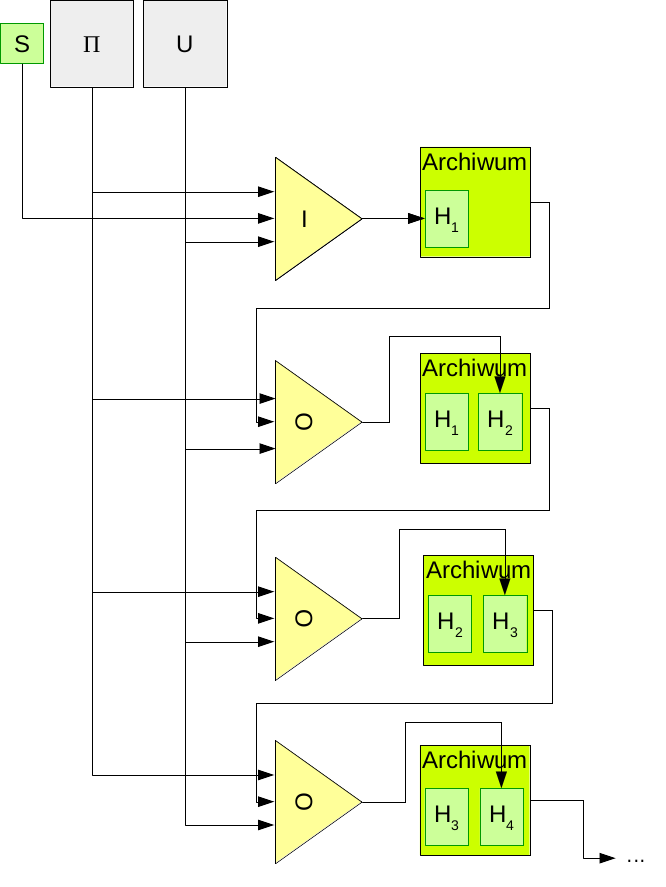
\includegraphics[scale=0.5]{img/ModelArchiwumFIFO2}\end{center}
\caption{Działanie heurystycznego algorytmu optymalizacyjnego z oknem archiwum wielkości równej dwukrotności osobników generowanych przez pojedynczą iterację. Zastosowano okno archiwum będące kolejką FIFO.}
\label{ModelArchiwumImg}
\end{figure}

\par{
I tak na przykład w opisanym w rozdziale \ref{DEvol_section} klasycznym algorytmie ewolucji różnicowej, mamy do czynienia z archiwum o rozmiarze równym wielkości populacji. Oznacza to, że do przeprowadzenia iteracji $N+1.$ algorytmu, oprócz $\Pi$ oraz $U$ potrzebujemy także wyniku $N.$ iteracji, ale już nie wyniku iteracji $N-1$. a tym bardziej całego archiwum $H$.
}
\par{
Tego rodzaju ograniczenia w wykorzystywaniu archiwum $H$ skłaniają do rozważań nad możliwością i stosownością wykorzystania informacji lub przesłanek ukrytych w nieużywanej części archiwum do poprawienia funkcjonowania algorytmu. W dziedzinie algorytmów heurystycznych, nie jest koncepcją nową [IGdzieŹródło] by parametryzować wykorzystywaną wielkość okna archiwum -- umożliwiając w ten sposób strojenie algorytmu oraz poprawianie jakości uzyskiwanych rezultatów. Pojawia się więc przypuszczenie, że także w przypadku ewolucji różnicowej powiększenie wykorzystywanego okna archiwum może umożliwiać uzyskiwanie lepszych jakościowo wyników optymalizacji.
}


%%%%% Ewolucja różnicowa
\section{Ewolucja różnicowa}
\label{DEvolChapter}

%%%%% Standard Evol
\subsection{Algorytmy z grupy ewolucyjnych}
\par{
Przykładem algorytmów heurystycznych stosowanych do rozwiązywania problemu optymalizacyjnego są algorytmy należące do grupy algorytmów ewolucyjnych (ang. \emph{Evolutionary Algorithms} -- AE) \cite{WykladyEvol,SpringerIntroToEvol}. Algorytmy te, wzorowane na ewolucji naturalnej operują pojęciami takimi jak osobnik, środowisko czy przystosowanie w celu adaptacyjnego przeszukiwania przestrzeni optymalizacyjnej.
}
\par{
Ogólna idea stojąca za algorytmami ewolucyjnymi, polega na opisaniu genotypu osobników, z których następnie można odczytać fenotyp (stanowiący punkt przestrzeni przeszukiwań) oceniany przez środowisko (funkcję optymalizowaną). Osobniki -- podobnie jak osobniki w naturze -- podlegają krzyżowaniu oraz niewielkim mutacjom, walcząc między sobą o zasoby naturalne. Zgodnie z teorią doboru naturalnego, osobniki gorzej dostosowane do środowiska są -- w szerokiej perspektywie czasowej i przy odpowiednio dużej populacji -- wypierane przez te dostosowane lepiej.
}
\par{
W związku z powyższą analogią w ramach algorytmów ewolucyjnych wyróżnia się następujące operatory:
\begin{description}
  \item[Krzyżowanie] -- to operator opisujący w jaki sposób na podstawie genotypu dwóch lub więcej osobników wytworzyć genotyp jednego lub więcej osobnika potomnego.
  \item[Mutacja] -- to operator wprowadzający w genotypie wybranego osobnika losowe (nieznaczne) zabużanie.
  \item[Selekcja] -- to operator odpowiadający selekcji naturalnej, który oceniając osobniki na podstawie przystosowania ich fenotypu do środowiska odrzuca część z nich preferując pozostawienie w populacji osobników lepiej dostosowanych.
  \item[Dobór do krzyżowania] -- to operator wybierający zestawy osobników podlegające krzyżowaniu. Operator ten opisuje znany z natury mechanizm preferencji (fenotypowej) organizmów przy rozmnażaniu.
  \item[Dobór do mutacji] -- to operator wybierający, które spośród osobników w populacji należy poddać mutacji. Odpowiada on zmiennemu w zależności od fenotypu organizmu prawdopodobieństwu wystąpienia u niego mutacji.
  \item[Inicjalizacja] -- to operator nieco oderwany od teorii ewolucji (gdyż ta nie opisuje powstawania pierwszych organizmów) opisujący sposób wygenerowania populacji początkowej spośród wszystkich możliwych genotypów. Operując na nomenklaturze z modelu opisanego w rozdziale \ref{Model}, operator ten jest funkcją przeprowadzającą zbiór punktów początkowych $S$ w początkowy zbiór genotypów.
  %%% dopasowanie do zakresu
\end{description}
}
\par{
Ogólny schemat działania algorytmu ewolucyjnego opiera się o iteracyjną adaptację populacji aż do ustalonego warunku stopu, według następujących kroków:
\begin{algorithm}[H]
\caption{Podstawowy schemat algorytmów ewolucyjnych}
\label{algorithm:ea}
\begin{algorithmic}[1]
\Function{Ewolucja}{$S$, $U$, $f$}
\State P $\gets$ $S$
	\While{!stop}
		\State C $\gets$ \Call{DoborDoKrzyzowania}{P, $U$, $f$}
		\State P $\gets$ P $\cup$ \Call{Krzyzowanie}{C, $U$}
		\State M $\gets$ \Call{DoborDoMutacji}{P, $U$, $f$}
		\State P $\gets$ P $\cup$ \Call{Mutacja}{M}
		\State P $\gets$ \Call{Selekcja}{P, $U$, $f$}
	\EndWhile
    \State \Return $argmin_{x \in X} f(x)$
\EndFunction
\end{algorithmic}
\end{algorithm}
}
\par{
W tym miejscu warto nadmienić, że choć w powyższym opisie algorytmów ewolucyjnych jest wprost mowa o podziale na genotyp i fenotyp, to na potrzeby zdefiniowanego problemu pojęcie fenotypu będzie wystarczające. Algorytmy opierające się o operacje na zakodowanym genotypie oderwanym od jego semantyki stanowią odrębną gałąź algorytmów ewolucyjnych i są nazywane algorytmami genetycznymi. Algorytmy te, ze względu na specyfikę swojego działania wymagają odpowiedniej reprezentacji danych i odpowiednio dobranych do reprezentacji operatorów. W przypadku rozważanego w pracy problemu optymalizacji, operowanie bezpośrednio na fenotypie ocenianym przez środowisko (a więc wektorach liczb rzeczywistych dla których wyznaczane są wartości funkcji optymalizowanej) ze względu na właściwości i możliwości samych liczb rzeczywistych wydaje się być w zupełności wystarczające. Zagadnienie podziału na genotyp i fenotyp będzie w dalszej części pracy zaniedbane.
}
\subsubsection{Eksploracja i Eksploatacja}
\par{
Ważnymi pojęciami opisującymi sposób w jaki osobniki w ramach algorytmów ewolucyjnych przeszukują przestrzeń są pojęcia \textbf{eksploracji} i \textbf{eksploatacji}. Definiują one dwutorowe działanie grup osobników:
\begin{description}
  \item[Eksploracja] -- to proces poszukiwania nowych, przyciągających osobniki obszarów przestrzeni przeszukiwań charakteryzujących się niską wartością funkcji przystosowania. Pojęcie to opisuje proces poszukiwania w całej przestrzeni obszarów przyciągania wielu minimów lokalnych. 
  \item[Eksploatacja] -- to proces badania obszaru przestrzeni przeszukiwań charakteryzującego się niską średnią wartością funkcji przystosowania. Pojęcie to opisuje proces poszukiwania minimum lokalnego przez punkty zawierające się w jego obszarze przyciągania.
\end{description}
}
\par{
Uzyskanie właściwego balansu między tymi dwoma aspektami działania algorytmów ewolucyjnych jest kluczowe dla powodzenia algorytmu ewolucyjnego. Efekt sterowania siłą dwóch charakterystyk przeszukiwań otrzymuje się, przez odpowiednie definiowanie operatorów oraz ich parametrów. W szczególności, zadaniem operatora krzyżowania jest przede wszystkim prowadzenie populacji w kierunku eksploatacji, natomiast zadaniem mutacji jest generowanie punktów poza w danej chwili badanym obszarem przyciągania - a więc eksploracja przestrzeni przeszukiwań. Istotnym elementem regulującym tę równowagę jest także operator selekcji, której charakter znacząco wpływa na przeżywalność i siłę przyciągania osobników pionierów (wygenerowanych losowo, nielicznych punktów, w nowym, atrakcyjnym obszarze przyciągania).
}

%%%%% Podstawowy DE
\subsection{Klasyczny algorytm ewolucji różnicowej}
\label{DEvol_section}
\par{
Szczególnym przypadkiem algorytmu należącego do grupy algorytmów ewolucyjnych są algorytmy ewolucji różnicowej (ang.\emph{ differential evolution}, DE). Algorytmy te, zbudowane są w sposób zakładający ich wykorzystanie do przeszukiwania przestrzeni ciągłej co jest zgodne z przyjętą we wstępie definicją problemu. Ich specyfika zakłada wykorzystanie do operatora mutacji odpowiednio przeskalowanych wektorów przesunięć wygenerowanych z bieżącej populacji punktów (Rysunek \ref{DEvolMutationBasic}) \cite{SpringerIntroToEvol}.
}

%%%%% Rysunek: Mutacja w DE
\begin{figure}[h]
\begin{center}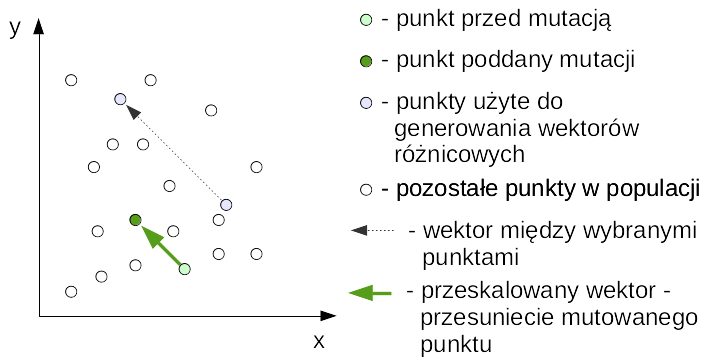
\includegraphics[scale=0.8]{img/BasicMutationSchema.png}\end{center}
\caption{Schemat działania operatora mutacji w ewolucji różnicowej na przykładzie przestrzeni dwuwymiarowej.}
\label{DEvolMutationBasic}
\end{figure}


\par{
Zgodnie z tą zasadą schemat ewolucyjny w populacji o indeksie ${t}$ -- $\mathbf{X^t}$, składa się z następujących kroków:
}

%%%%% BAZOWY SCHEMAT DE
\par{
	\begin{description}
	
	
  		\item[Generowanie mutantów]:\\
  Ten krok polega na wygenerowaniu z wektora osobników mutantów $\mathbf{V^{t}}$ o długości równej wielkości populacji - tak by każdemu osobnikowi $\mathbf{x_i^{t}}$ odpowiadał osobnik mutant $\mathbf{v_i^{t}}$.
  Do tego celu wykorzystywane są wybrane z populacji punkty - punkt mutowany oraz punkty wymagane do wygenerowania wektorów różnicowych. W najbardziej klasycznym wariancie algorytmu wszystkie te punkty są dla każdego $i$ generowane losowo \cite{SpringerIntroToEvol} (oznaczamy $r_1, r_2, r_3$).
  W opisanym wariancie $\mathbf{v_i^{t}}$ wyznaczane jest jako:

%%%%%% Podstawowe równanie mutacji różnicowej
\begin{equation} \label{eq:DiffMutation}
 \mathbf{v_i^{t}} = \mathbf{r_1} + F \cdot (\mathbf{r_2} - \mathbf{r_3})
\end{equation}

Gdzie $F$ to rzeczywistoliczbowy współczynnik skalujący najczęściej należący do przedziału $[0, 1]$. Literatura \cite{SpringerIntroToEvol} podaje również że w podstawowym wariancie ewolucji różnicowej zachodzi:
\begin{equation}
\mathbf{x_1^{t}} \neq \mathbf{r_1} \neq \mathbf{r_3} \neq \mathbf{r_3}
\end{equation}
nie jest to jednak warunek wymagany dla każdego algorytmu tej klasy.


	  \item[Krzyżowanie]:\\
  W tym kroku każdy z osobników w populacji $\mathbf{X^{t}}$ jest krzyżowany z odpowiadającym mu osobnikiem z populacji mutantów $\mathbf{V^{t}}$ w celu wyłonienia osobnika dziecka $\mathbf{z_i^{t}}$ dla każdego osobnika $\mathbf{x_i^{t}}$. Choć do krzyżowania można stosować wiele różnych operatorów, najczęściej wybierane jest krzyżowanie wymieniające z różnym rozkładem prawdopodobieństwa. W najprostszym wypadku dwumianowy wymieniający operator krzyżujący (ang. \emph{binominal crossover}) może być zdefiniowany następująco:
  
%% Krzyzowanie BIN
\begin{equation}
\label{eq:BasicCrossover}
z_{i,j}^{t} = \left\{ \begin{array}{ll}
v_{i,j}^{t} & \textrm{gdy $r \le Cr$}\\
x_{i,j}^{t} & \textrm{w przeciwnym wypadku}\\
\end{array} \right.
\end{equation}
Gdzie:
\begin{itemize}
\item $r$ -- zmienna losowa o rozkładzie jednostajnym na przedziale [0, 1]
\item $Cr$ -- współczynnik krzyżowania, parametr algorytmu z dziedziny [0, 1]
\end{itemize}
Wartym odnotowania jest konieczność zapewnienia by do każdego osobnika dziecka $\mathbf{z_i^{t}}$ trafiła co najmniej jedna wartość z osobnika mutanta, a więc by zachodziło $\mathbf{z_i^{t}}~\neq~\mathbf{x_i^{t}}$ \cite{SpringerIntroToEvol}. Ze względu na prostotę zapisu element ten zaniedbano jednak w powyższej definicji.


		\item[Selekcja]:\\
Ostatnim elementem podstawowej strategii ewolucyjnej dla algorytmów ewolucji różnicowej jest wybór osobników spośród par $(\mathbf{x_i^{t}}, \mathbf{z_i^{t}})$. Wybór ten w typowym przypadku dokonywany jest wg. następującej formuły:
\begin{equation}
\mathbf{x_{i}^{t+1}} = \left\{ \begin{array}{ll}
\mathbf{v_{i}^{t}} & \textrm{gdy $f(v_i^t) \le f(x_i^t)$}\\
\mathbf{x_{i}^{t}} & \textrm{w przeciwnym wypadku}\\
\end{array} \right.
\end{equation}
Tego rodzaju podejście stanowi o elitarności wyboru osobników do kolejnych pokoleń, co powoduje zwiększenie możliwości eksploatacyjnych algorytmu kosztem jego możliwości eksploracyjnych.
\end{description}
}

\par{
Działanie algorytmu ewolucji różnicowej zdeterminowane jest przez zestaw operatorów (opisane niżej) jak również podstawowe parametry:
\begin{itemize}
\item $\mu$ - liczebność populacji - określa ile osobników zostanie stworzonych we wstępnej fazie algorytmu i ile z nich przetrwa na końcu każdego pokolenia.
\item $Cr$ - współczynnik krzyżowania określający (w przypadku wariantu \emph{bin}) prawdopodobieństwo wybrania każdego z elementów osobnika mutanta do osobnika dziecka, jak w równaniu \ref{eq:BasicCrossover}.
\item $F$ - współczynnik skalujący wektor przesunięcia punktu w populacji.
\end{itemize}
}

\par{
Podsumowując działanie klasycznego algorytmu ewolucji różnicowej można można posłużyć się poniższym pseudokodem, operującym na wprowadzonych w rozdziałach \ref{Model} i \ref{DEvol_section} symbolach:
\begin{algorithm}[H]
\caption{Klasyczny algorytm ewolucji różnicowej -- \emph{DE}/\emph{rand}/\emph{1}/\emph{bin}}
\label{algorithm:de}
\begin{algorithmic}[1]
\Function{EwolucjaRoznicowa}{$S$, $U$, $f$, $\mu$, $Cr$, $F$, $\mu$}
    \State X = $S$
    \While{!stop}
	    \State V $\gets$ \Call{Mutacja}{X, $\mu$, $U$, $F$}
        \State Z $\gets$ \Call{Krzyzowanie}{X, V, $\mu$, $U$, $Cr$}
        \State X $\gets$ \Call{Selekcja}{Z, X, $\mu$, $f$}
    \EndWhile
    \State \Return $argmin_{x \in X} f(x)$
\EndFunction
\State
\Function{Mutacja}{X, $\mu$, $U$, $F$}
    \ForAll{i $\in$ 1:$\mu$}
    	\State V[i] $\gets$ X[$U_\mu$] + $F \cdot $(X[$U_\mu$] - X[$U_\mu$])
    \EndFor
    \State \Return V
\EndFunction
\State
\Function{Krzyzowanie}{X, V, $\mu$, $U$, $Cr$}
    \ForAll{i $\in$ 1:$\mu$}
        \ForAll{j $\in$ 1:D}
            \If{$Cr < U_u$}
                \State Z[i][j] $\gets$ V[i][j]
            \Else
                \State Z[i][j] $\gets$ X[i][j]
            \EndIf
        \EndFor
    \EndFor
    \State \Return return Z
\EndFunction
\State
\Function{Selekcja}{Z, X, $\mu$, $f$}
    \ForAll{i $\in$ 1:$\mu$}
        \If{$f($Z$) \le f($X$)$}
            \State $X_{new}$[i] $\gets$ Z[i]
        \Else
            \State $X_{new}$[i] $\gets$ X[i]
        \EndIf
    \EndFor
    \State \Return $X_{new}$
\EndFunction
\end{algorithmic}
\end{algorithm}

Dla uproszczenia zapisu jako $U_\mu$ oznaczono liczbę losową wygenerowaną z przestrzeni $U$, z równym prawdopodobieństwem ze zbioru $[1, \mu] \cap \mathbb{N}$. Symbolem $U_u$ oznaczono natomiast liczbę losową wygenerowaną z przestrzeni $U$ z rozkładem $U(0,1)$.
}

\subsection{DE a klasyczne strategie ewolucyjne}
\par{
Podstawową różnicą w stosunku do klasycznych strategii ewolucyjnych jest nietypowy schemat mutacji i ścisły dobór par poddawanych krzyżowaniu tak, by zawsze stanowiły one kombinację mutanta i osobnika z populacji  podstawowej.
}
\par{
Ponadto, ważnym elementem tego algorytmu jest także fakt, że wykorzystuje on zawartą w populacji informację o uzyskanych dotąd przesłankach na temat kształtu badanej funkcji. W klasycznych algorytmach ewolucyjnych, sposób rozłożenia populacji w przestrzeni determinuje typowo jedynie punkty bazowe dla nowej populacji. W przypadku ewolucji różnicowej, nowe punkty generowane z populacji podlegają wyciągnięciu w kierunkach, w których przeszukiwanie przyniosło lepsze rezultaty. Pozwala to na szybsze poruszanie się populacji w adaptującym się do bieżącego krajobrazu kierunku i prędkości.
}
\par{
Warto także zwrócić uwagę, że algorytmy ewolucji różnicowej mają zwykle bardziej elitarny charakter selekcji niż klasyczne algorytmy ewolucyjne, powoduje to częstszą zbieżność populacji do pojedynczych punktów w przestrzeni a także przyspiesza przejście algorytmu w fazę ekspoatacji. Fakt ten dodatkowo potęguje typowy wybór wartości $F \in [0, 1]$, który powoduje geometryczne zmniejszanie się średniej długości wektora różnicowego wraz z upływem pokoleń, w przypadku przejścia algorytmu w fazę eksploatacji pojedynczego punktu.
}
\par{
Co do zasady algorytmy ewolucji różnicowej stanowią cenny punkt wyjścia dla dalszych rozważań, ponieważ już przy bardzo prostych operatorach pozwalają na uzyskiwanie bardzo dobrych właściwości eksporacyjnych i eksploatacyjnych.
}

\subsection{Podstawowe warianty ewolucji różnicowej}
\subsubsection{Ilość par różnicowanych}
\par{
Opisany wyżej standardowy schemat ewolucji różnicowej, jest wersją podstawową, której zachowanie można na wiele sposobów zmodyfikować, pozostając nadal w tej klasie algorytmów. Podstawowa różnica jaką mogą charakteryzować się poszczególne instancje DE, to ilość par wykorzystywanych do mutacji różnicowej. W ewolucji różnicowej uogólnionej ze względu na ilość różnicowanych par, krok mutacji różnicowej (\ref{eq:DiffMutation}) zostaje zamieniony na \cite{PracticalInsights}:
\begin{equation}
\mathbf{v_i^{t}} = \mathbf{r_1} + \sum_{d = 1}^D F_d \cdot (\mathbf{r_{j,1}} - \mathbf{r_{j,2}})
\end{equation}
gdzie jako $D$ oznaczono ilość elementów poddawanych mutacji różnicowej.
}
\par{
W praktyce, najczęściej stosuje się $D = 1$ lub $D = 2$ i $F_1 = F_2$, ponieważ nie znaleziono przesłanek by dalsze zwiększenie wartości $D$ powodowało poprawę jakości otrzymywanych przy użyciu algorytmu wyników \cite{PracticalInsights}.
\subsubsection{Schemat mutacji}
\par{
Najistotniejszą z punktu widzenia charakterystyki DE możliwością zmodyfikowania zachowania algorytmu jest możliwość, zamiany schematu mutacji. Podstawowy schemat mutacji (\emph{rand}) zakłada losowanie osobników $\mathbf{r_1}, \mathbf{r_2}, \mathbf{r_3}$ i postępowanie wg schematu \ref{eq:DiffMutation}. W ramach licznych badań powstała jednak znaczna ilość wariantów bardziej wysublimowanych. Najpopularniejsze w literaturze i najistotniejsze ze względu na zawartość pracy schematy mutacji to:
\begin{description}

\item[rand] \cite{RainerStorn,SpringerIntroToEvol} -- wariant podstawowy
\item[best] \cite{PracticalInsights} -- ten schemat zakłada zmianę schematu \ref{eq:DiffMutation} na:
\begin{equation}
\mathbf{v_i^{t}} = \mathbf{x_{best}^t} + F \cdot (\mathbf{r_{1}} - \mathbf{r_{2}})
\end{equation}
gdzie $\mathbf{x_{best}^t}$ to osobnik z populacji $t$, który uzyskał najlepszy wynik oceny funkcją $f$. Schemat ten, promuje poszukiwanie rozwiązania wokół najlepszego dotychczas znalezionego osobnika, wedle rozrzutu bieżącej populacji. Pozwala to na adaptacyjne skupienie się populacji wokół lokalnego optimum i eksploatowanie jego możliwości, kosztem możliwości eksploracyjnych algorytmu.
\item[mid] \cite{DEmid} -- ten schemat zakłada zmianę schematu \ref{eq:DiffMutation} na:
\begin{equation}
\mathbf{v_i^{t}} = \mathbf{x_{mid}^t} + F \cdot (\mathbf{r_{1}} - \mathbf{r_{2}})
\end{equation}
gdzie $\mathbf{x_{mid}^t}$ to punkt środkowy populacji $t$ zdefiniowany jako:
\begin{equation}
x_{mid,j}^t = \frac{1}{n}\sum_{i=1}^n{x_{i,j}}
\end{equation}
gdzie $n$ to wielkość populacji. Schemat ten został opracowany niedawno i czerpie on swoją inspirację z podejrzenia o informacji niesionej przez środek populacji. Koncepcja ta zostanie rozwinięta w rozdziale \ref{MidPoint}.

\item[current-to-rand] \cite{PracticalInsights} -- ten schemat zakłada zmianę schematu \ref{eq:DiffMutation} na:
\begin{equation}
 \mathbf{v_i^{t}} = K \cdot \mathbf{x_i^t} + (1 - K) \cdot \mathbf{r_{1}} + F \cdot (\mathbf{r_{2}} - \mathbf{r_{3}})
\end{equation}
W tym schemacie do standardowego schematu \emph{rand} dołącza się element wiążący mutanta ze sparowanym z nim osobnikiem z populacji podstawowej $\mathbf{X}$. Wykorzystuje się w tym celu zmienną $K \in [0, 1]$, która stanowi wagę dla osobnika z populacji podstawowej $\mathbf{x_i^t}$. W praktyce oznacza to, że mutant $\mathbf{v_i^t}$ powstaje przez przesunięcie punktu leżącego między $\mathbf{x_i^t}$ a losowo wybranym punktem z populacji $\mathbf{r_1}$ o przeskalowany współczynnikiem $F$ wektor między dwoma losowymi osobnikami z populacji (Rysunek \ref{current-to-rand-img}).

%%%%% Rysunek: current-to-rand
\begin{figure}[h]
\begin{center}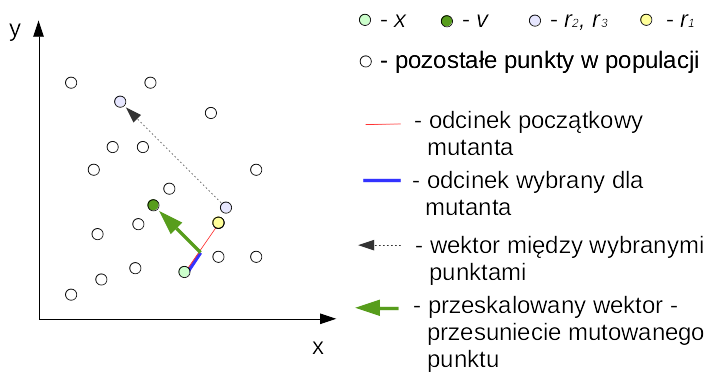
\includegraphics[scale=0.8]{img/current-to-rand-mutation.png}\end{center}
\caption{Schemat mutacji różnicowej \emph{current-to-rand} na przykładzie przestrzeni dwuwymiarowej. Jeśli czerwony odcinek ma długość $l$, to odcinek niebieski ma długość $l \cdot K$}
\label{current-to-rand-img}
\end{figure}


\item[current-to-best] \cite{PracticalInsights} -- ten schemat zakłada zmianę schematu \ref{eq:DiffMutation} na:
\begin{equation}
\mathbf{v_i^{t}} = K \cdot \mathbf{x_i^t} + (1 - K) \cdot \mathbf{x_{best}^t} + F \cdot (\mathbf{r_{1}} - \mathbf{r_{2}})
\end{equation}
Schemat ten jest analogiczny do schematu \emph{current-to-rand}, jednak oparty o przesłankę związaną z najlepszym punktem populacji. Procedura ta zakłada przesuwanie wygenerowanym wektorem punktu leżącego między odpowiadającemu danemu mutantowi osobnikiem z populacji podstawowej a punktem o najlepszej dotąd wartości funkcji optymalizowanej.


\item[rand-to-best] \cite{PracticalInsights} -- ten schemat zakłada zmianę schematu \ref{eq:DiffMutation} na:
\begin{equation}
\mathbf{v_i^{t}} = K \cdot \mathbf{x_{best}^t} + (1 - K) \cdot \mathbf{r_1} + F \cdot (\mathbf{r_{2}} - \mathbf{r_{3}})
\end{equation}
Schemat ten, podobnie jak dwa poprzednie, opiera się o przypuszczenie, że istnieje możliwość poprawienia skuteczności algorytmu przez zwiększenie rozrzutu punktów początkowych w przestrzeni przeszukiwań. W tym jednak wypadku, mamy do czynienia z połączeniem koncepcji znanych ze schematów \emph{rand} i \emph{best} w celu (w miarę możliwości) uzyskania najlepszych cech obu z nich. Warunki eksploracyjne tego schematu są poprawione względem schematu \emph{best}, ze względu na możliwość odciągania punktów od lokalnego optimum przez osobniki znajdujące się w okolicy innego optimum. Zarazem, w przypadku dotarcia przez algorytm do fazy czysto eksploatacyjnej (skupienie wokół jednego minimum całej populacji), możliwości eksploatacyjne schematu \emph{best} zostają zachowane.

\item[current-to-pbest] \cite{JADE} -- ten schemat zakłada zmianę schematu \ref{eq:DiffMutation} na:

\begin{equation}
\mathbf{v_i^{t}} = \mathbf{x_i^t} + F \cdot (\mathbf{x_{r_{pbest}}^t} - \mathbf{x_i^t}) + F \cdot (\mathbf{r_1} - \mathbf{r_{2}})
\end{equation}
gdzie $\mathbf{x_{r_{pbest}}^t}$ to osobnik wybrany losowo spośród $p \cdot n$ osobników o najniższej wartości funkcji optymalizowanej, $p \in (0,1]$. W niektórych pracach \cite{SHADE} proponowane jest dolne ograniczenie wartości $p$ jako $p_{min} = \frac{2}{\mu}$, co oznacza, że osobnik $\mathbf{x_{r_{pbest}}^t}$ jest zawsze losowany spośród co najmniej dwóch najlepszych osobników.

Rozwiązanie to ma za zadanie dołączyć do zalet schematu \emph{current-to-best} dodatkowe rozrzucenie osobników w przeszukiwanej przestrzeni i osłabienie siły przyciągania jednego najmocniejszego osobnika, a więc zmniejszenie elitaryzmu całego algorytmu.


\par{
Działanie poszczególnych operatorów mutacji zaprezentowano na rysunkach \ref{mutations1} i \ref{mutations2}.
}


\begin{figure}[h]
\begin{center}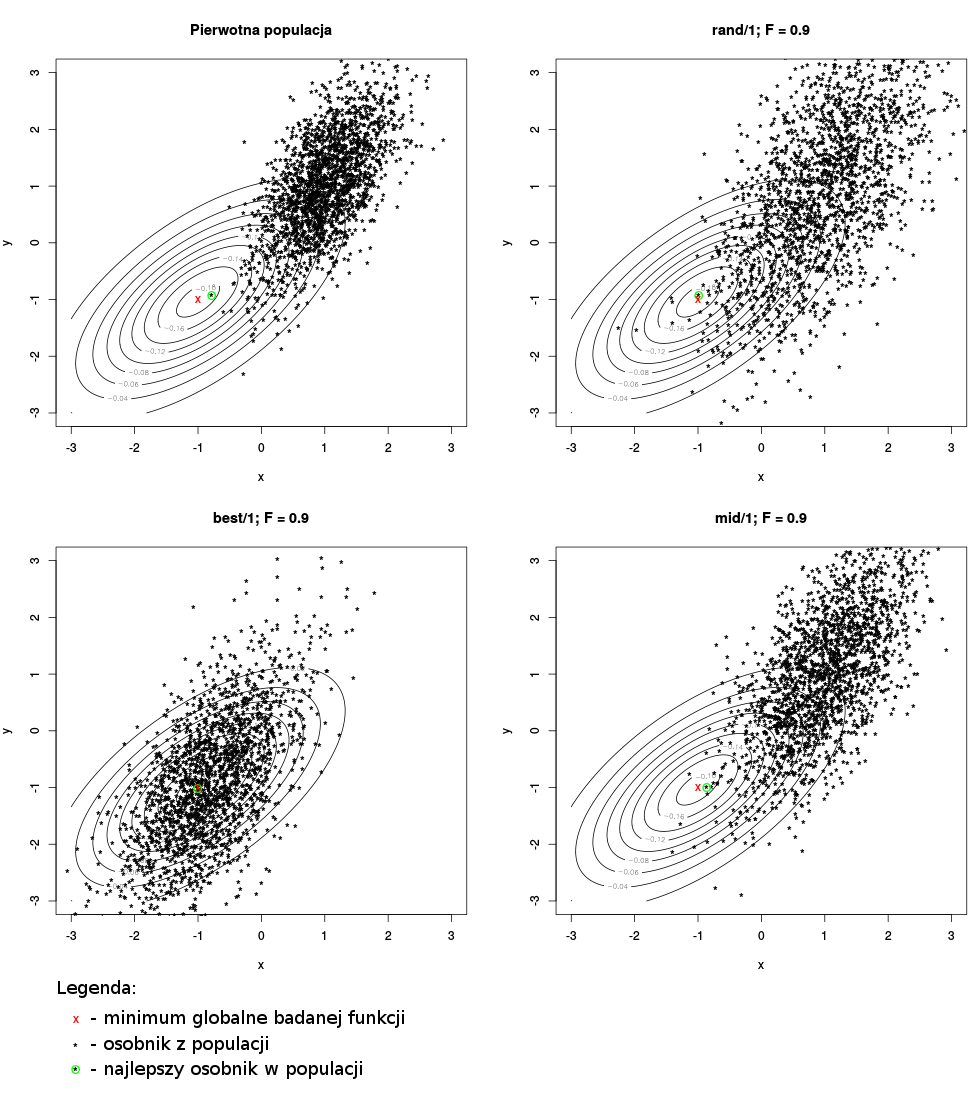
\includegraphics[scale=0.375]{img/mutations1.png}\end{center}
\caption{Działanie poszczególnych schematów mutacji różnicowej przy pokazanej populacji pierwotnej.}
\label{mutations1}
\end{figure}

\begin{figure}[h]
\begin{center}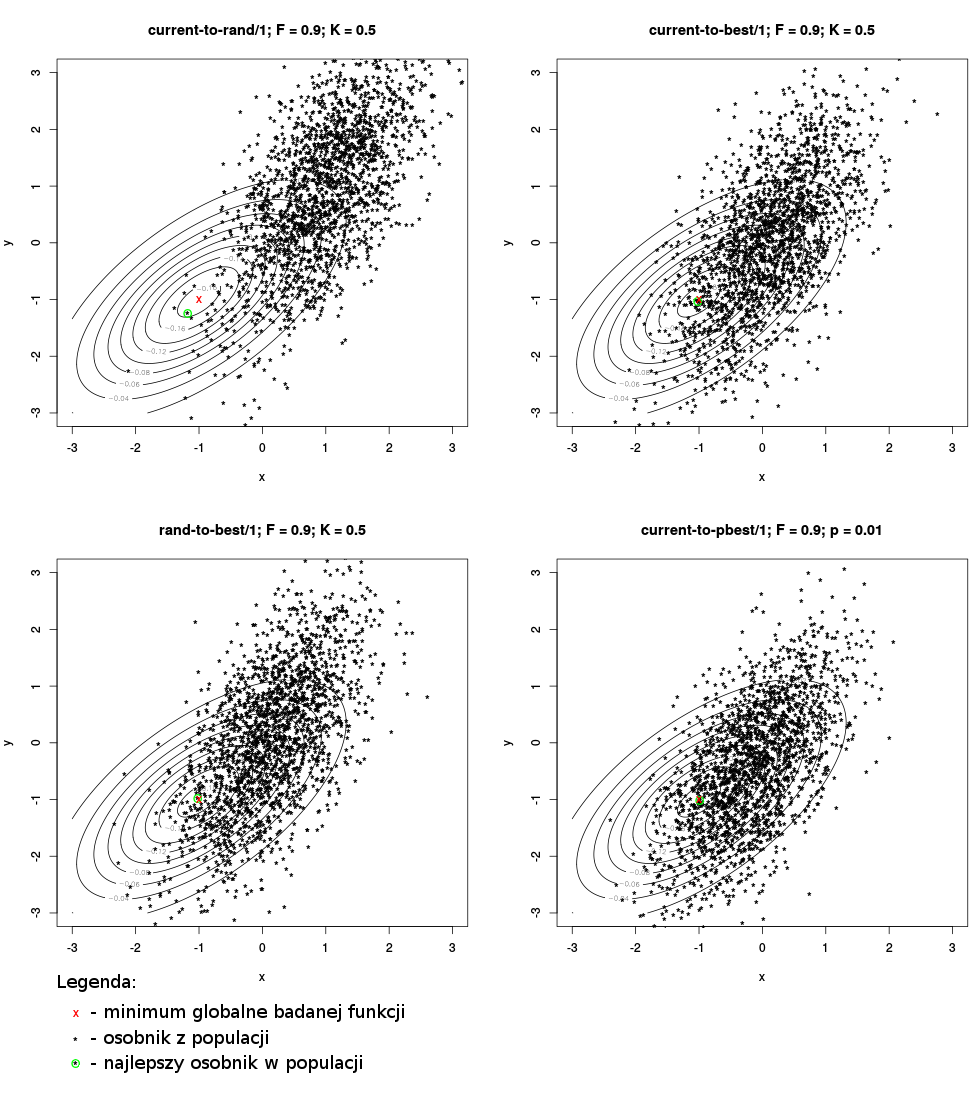
\includegraphics[scale=0.375]{img/mutations2.png}\end{center}
\caption{Działanie poszczególnych schematów mutacji różnicowej przy pokazanej na rysunku \ref{mutations1} populacji pierwotnej.}
\label{mutations2}
\end{figure}

\end{description}
}
\subsubsection{Schemat krzyżowania}
\par{
Krzyżowanie w klasycznym algorytmie ewolucji różnicowej, pełni kluczową rolę -- zapewnia powiązanie osobników mutantów z populacji $\mathbf{V}$ w pary z osobnikami z populacji bazowej $\mathbf{X}$. W ten sposób tworzy przyczynek do wykorzystywania par osobników do selekcji przez ich bezpośrednie porównanie. W bardziej wysublimowanych schematach mutacji opisanych w poprzednim podrozdziale, osobnik z bieżącej populacji bywa wykorzystywany już na etapie mutacji. Nie jest to regułą ani założeniem niezbędnym dla skonstruowania poprawnych operatorów dla ewolucji różnicowej, stąd też nawet w odbiegających od podstawowego wariantu wersjach algorytmów ewolucji różnicowej, krzyżowanie jest niezbędne dla poprawnego zachowania algorytmu.
}

\par{
Typowo w literaturze spotyka się następujące schematy krzyżowania:
\begin{description}
\item[bin] -- podstawowy schemat krzyżowania zgodny z równością \ref{eq:BasicCrossover}.
\item[exp] -- schemat krzyżowania zamieniający równość \ref{eq:BasicCrossover}, na procedurę:
\begin{algorithm}[H]
\caption{Schemat krzyżowania \textbf{exp}}
\label{algorithm:ea}
\begin{algorithmic}[1]
\State j $\gets$ 1
\While{r < $Cr$ $\land$ j $\le$ D}
	\State $z_{i,j}^t$ $\gets$ $v_{i,j}^t$
	\State j $\gets$ j + 1
\EndWhile
\While{j < D}
	\State $z_{i,j}^t$ $\gets$ $x_{i,j}^t$
\EndWhile
\end{algorithmic}
\end{algorithm}

Tego rodzaju krzyżowanie powoduje dążący (gdy $D \rightarrow \infty$) do wykładniczego rozkład położenia pierwszego elementu wektora pochodzącego z osobnika $\mathbf{x_i^t}$. Rozkład ten nie traktuje wszystkich pozycji w wektorze osobników identycznie, ponieważ dalsze pozycje w wektorze będą rzadziej zastępowane przez wartości z osobników mutantów. W związku z tym stosuje się także wariant, który wybiera ilość elementów ($n_x$) pochodzących z osobnika rodzica zgodnie z opisanym rozkładem a następnie wybiera z równym prawdopodobieństwem $n_x$ elementów wektora, które będą pochodziły z osobnika $\mathbf{x_i^t}$.
\end{description}
}
\subsubsection{Notacja}
\par{
Mając na względzie, że typowo algorytmy ewolucji różnicowej rozróżniane są między sobą na podstawie trzech wyżej wymienionych zmiennych - a więc: ilości par różnicowanych, schematu mutacji różnicowej i schematu krzyżowania, wprowadzono notację pozwalającą w sposób zwięzły opisać konkretną instancję algorytmu z grupy algorytmów ewolucji różnicowej \cite{PracticalInsights}:
%%%%%% Zapis 
\begin{center}
\textbf{DE/M/D/C}
\end{center}
gdzie:
\begin{itemize}
\item \textbf{M} - schemat mutacji (np. \emph{rand}, \emph{current-to-pbest}).
\item \textbf{D} - ilość par różnicowanych (zwykle \emph{1} lub \emph{2}).
\item \textbf{C} - schemat krzyżowania (np. \emph{bin}, \emph{exp}).
\end{itemize}
I tak na przykład klasyczny algorytm ewolucji różnicowej (\ref{DEvol_section}) wg tej notacji byłby opisany jako: DE/\emph{rand}/\emph{1}/\emph{bin}. Notacja ta będzie wykorzystywana w dalszej części pracy.
}


\subsection{Strategie adaptacji}
\label{Adaptation}
\par{
Dla każdego z opisanych schematów istnieją prace opisujące proces adaptacji parametrów na podstawie dotychczas uzyskiwanych rezultatów \cite{zhang2009adaptive,JADE,SHADE}. Nierzadko proces adaptacji wykorzystanie informacje historii $H$ o szerokości przekraczającej wielkość pojedynczego pokolenia stąd metody adaptacji mogą być traktowane jako jedna z prób poprawy działania algorytmów ewolucji różnicowej przez poszerzenie okna archiwum.
}
\par{
Opublikowane prace jednoznacznie wskazują, że proces adaptacji znacząco poprawia uzyskiwane w ramach ewolucji różnicowej wyniki. Stanowi to kolejną przesłankę pozwalającą oczekiwać poprawy rezultatów przez wykorzystanie szerszego okna historii.
}
\par{
Dodatkowo należy odnotować, że adaptacyjne algorytmy ewolucyjne otrzymują najlepsze rezultaty w testach typu \emph{black-box} (spośród algorytmów klasy DE) \cite{CEC2013Comp}. Fakt ten staje się przyczynkiem do tego by sprawdzić, czy proponowany algorytm \emph{NADE} będzie utrzymywał swoją charakterystykę jakości także względem tych modyfikacji.
}

\subsection{Punkt środkowy populacji}
\label{MidPoint}
\par{
Niedawno w badaniach nad algorytmami ewolucji różnicowej \cite{DEmid} pojawiła się koncepcja wykorzystania inforamcji niesionej przez punkt środkowy populacji do poprawy sposobu działania algorytmu. W pracy \cite{DEmid} podjęto próbę zbudowania nowego schematu mutacji, w którym punktem bazowym jest punkt środkowy populacji (DE/\emph{mid}/\emph{k}). Wnioskiem z tej pracy było stwierdzenie, iż dla większości funkcji zwłaszcza w wielowymiarowych przestrzeniach, wybór strategii \emph{mid} poprawia w sposób statystycznie istotny działanie algorytmu ewolucji różnicowej. W pracy zwrócono także uwagę, że punkt środkowy nie przynosi znaczącej poprawy lub wręcz jest mylący dla zadania, w przypadku pewnych funkcji. Jako przykład takiej funkcji wymieniono funkcję Weierstrassa wchodzącą w skład zestawu testowego CEC2013 (\ref{CEC2013chapter}).
}
\par{
Praca ta jednoznacznie wskazała, że informacja zawarta w punkcie środkowym dla wielu problemów może być użyteczna. Intuicja podpowiada, że w szczególności w fazie eksploatacji okolic lokalnego optimum punkt środkowy może być o wartości wyższej niż najlepsza. Taka własność punktu środkowego stanowiła by wytłumaczenie przewagi algorytmu DE/\emph{mid}/\emph{1} nad DE/\emph{best}/\emph{1}. Choć początkowo zamierzano włączyć w skład pracy badanie dotyczące tej tezy, to ze względu na dużą ilość innych tez wymagających sprawdzenia w ostatecznej wersji rezygnowano z badania tej tezy.
}
\subsection{Metoda uwzględniania ograniczeń}
\par{
Praca \cite{Boundary}, pokazała że metoda uwzględniania ograniczeń przeszukiwanej przestrzeni ma istotny wpływ na jakość rezultatów uzyskiwanych przez algorytm ewolucji różnicowej. Praca wyszczególnia wiele typów dopasowywania punktów mutantów do zakresu:
\begin{description}
\item[Reinicjalizacja] (ang. \emph{Reinitialization} -- Powszechnie używana w algorytmach ewolucji różnicowej strategia \cite{Boundary}, która polega na zamianie punktu, który znalazł się poza ograniczeniami, na losowo wybrany (z rozkładem jednostajnym) punkt mieszczący się w ograniczeniach.
\item[Ponowne próbkowanie] (ang. \emph{Resampling}) -- Metoda, która okazała się bardzo skuteczna, w szczególności w przypadku dużej ilości punktów nie mieszczących się w ograniczeniach. Polega ona na powtarzaniu procedury tworzenia mutanta na podstawie losowych wektorów różnicowych, do czasu osiągnięcia osobnika, który mieści się w ograniczeniach.
\item[Odbijanie] (ang. \emph{Reflection}) -- Metoda polegająca na odbijaniu punktu względem wszystkich przekroczonych linii ograniczeń aż do czasu, gdy punkt znajdzie się wewnątrz przeszukiwanego obszaru przestrzeni.
\item[Rzutowanie] (ang. \emph{Projection}) -- Metoda ta polega na rzutowaniu prostopadłym punktu na wszystkie przekroczone ograniczenia.
\item[Zawijanie] (ang. \emph{Wrapping}) -- w tej metodzie, zakłada się, że obszar przeszukiwań jest skończonym wycinkiem hiperpłaszczyzny. Mając to na względzie, nakłada się tą skończoną podprzestrzeń na hipertorusa w ten sposób zyskując przestrzeń posiadającą wyłącznie punkty dopuszczalne a opisującą cały zbiór $\mathbb{R}^D$. Wadą tego rozwiązania jest fakt, że jeśli funkcja $f$ jest ciągła, to jej w nowej przestrzeni jej ciągłość może zostać zerwana.
\item[Zachowywanie] (ang. \emph{Conservatism}) -- metoda ta polega na odrzuceniu dziecka $z_i$ jeśli znajdzie się ono poza obszarem przeszukiwania i w czasie selekcji wybranie osobnika $x_i$. Podejście to jest równoważne nadaniu funkcji kary za przejście poza granicę obszaru przeszukiwania, równej $\infty$ w każdym punkcie poza ograniczeniami.
\end{description}
}
\par{
Wyniki otrzymane w ramach \cite{Boundary} sugerują, że najlepiej sprawdzają się metodą uwzględniania ograniczeń jest \emph{resampling}. Poważnymi wadami tego rozwiązania jest znaczne skomplikowanie struktury algorytmu, ze względu na konieczne nawroty, a także koszta wynikające z dodatkowych obliczeń (zwłaszcza w przypadku dużego odsetka odrzucanych punktów). Z tych powodów zdecydowano, by odrzucić tę metodę i na czas pracy skorzystać z jednej z dwóch znacznie prostszych a dających podobne, obiecujące rezultaty -- \emph{odbijania} i \emph{rzutowania}. Spośród tych dwóch wariantów arbitralnie wybrano \emph{odbijanie} i ten sposób uwzględniania ograniczeń będzie wykorzystywany przy wszystkich testach w ramach pracy.
}

\subsection{Archiwum}
\label{ArchiveLiterature}
\par{
W literaturze spotyka się niezliczone próby jawnego lub niejawnego wykorzystania dodatkowego archiwum w algorytmach ewolucji różnicowej. Poniżej opisano podejście do archiwum w kilku pracach, które w jawny sposób powołują się na poprawę jakości działania algorytmu ewolucji różnicowej dzięki zastosowaniu archiwum. Niestety żadna z tych prac nie bada skuteczności archiwum w oderwaniu od innych metod usprawniania algorytmów.
}
\subsubsection{Archiwum w ADE \cite{ArchivedDE,RobustArchiveDE}}
\par{
W pracy \cite{ArchivedDE} opracowano algorytm \emph{ADE} (ang. \emph{Archived Differential Evolution}) wykorzystujący archiwum mające przechowywać informacje o najlepszych osobnikach we wszystkich następujących po sobie pokoleniach. Archiwum tego rodzaju pełniło w algorytmie trzy funkcje:
\begin{description}
\item[Wskaźnika wysycenia konkretnej populacji] -- przyjęto tu założenie, że jeśli najlepszy punkt w populacji nie zmienił się od pewnej definiowalnej ilości pokoleń, należy przyjąć, że obecna populacja nie ma perspektyw na odnalezienie znacząco lepszych punktów. W algorytmie \emph{ADE} był to jeden z warunków wyzwalających adaptację populacji.
\item[Wskaźnika zbliżenia się populacji do lokalnego optimum] -- w algorytmie podjęto próbę wykorzystania informacji zawartych w punkcie środkowym populacji. Jednym z warunków wyzwalających adaptację populacji, było bowiem zmniejszenie odległości euklidesowej:
\begin{equation}
d = \sqrt{\sum_{i = 1}^{D}(x_{best,i} - x_{mean,i})^2}
\end{equation}
gdzie $\mathbf{x_{mean}}$ stanowi punkt środkowy populacji definiowany jako:
\begin{equation}
x_{mean,i} = \frac{1}{\mu} \cdot \sum_{j = 1}^{\mu}x_{j,i}
\end{equation}
Wspomniany warunek wyrażony jest jako:
\begin{equation}
d \le \epsilon
\end{equation}
gdzie $\epsilon$ to parametr algorytmu określający graniczną odległość między wspomnianymi punktami.
Jeśli warunek jest spełniony, następuje adaptacja populacji.
\item[Punktu odniesienia dla adaptacji populacji] -- w algorytmie w wyniku kilku warunków następowała adaptacja popualacji mająca na celu poprawę właściwości eksporacyjnych algorytmu. Adaptacja odbywała się wg. formuły zmieniającej osobniki w populacji \cite{ArchivedDE}:
\begin{equation}
x_{i,j,G} = \lambda \cdot x_{i,Best,A} + (1 - \lambda) \cdot (x_{i,Best,A} - x_{i,j,G-1})
\end{equation}
gdzie $\lambda \sim U[0,1]$ natomiast $x_{i,j,G}$ oznacza wartość $i$ elementu wektora osobnika $j$ w populacji $G$, a $x_{i,Best,A}$ oznacza wartość $i$ elementu wektora najlepszego osobnika w archiwum.
\end{description}
}
\par{
Poważną wadą samego algorytmu jest wykorzystywanie informacji wykraczających poza te pozyskiwalne z definicji (rozdział \ref{ProblemDefinition}). W szczególności algorytm wykorzystuje trudności opisane w rozdziale \ref{WadyBB} wykorzystując parametr $\epsilon$ a nawet sugerując jego uniwersalną arbitralną wartość $10^{-3}$. Tego rodzaju podejście przeczy założeniom opisywanego problemu.
}
\par{
Algorytm \emph{ADE} został przez autorów oceniony pozytywnie w kontekście badanych problemów. Wykorzystuje on jednak archiwum w niewielkim stopniu a ponadto nie bada tego zastosowania w odcięciu od pozostałych technik poprawy jakości działania algorytmu. Sama metoda reinicjalizacji oparta o brak poprawy w kolejnych pokoleniach stanowi przykład przeniesienia znanych z innych algorytmów technik na grunt ewolucji różnicowej.
}

\subsubsection{Archiwum w CDDE{\_}Ar \cite{ClusterArchiveDE}}
\par{
Algorytm \emph{CDDE{\_}Ar} operaty jest o idee podzielenia populacji na mniejsze grupy (klastrowanie) przy użyciu algorytmu \emph{k-średnich} \cite{KMeans}. Tego rodzaju grupy, traktowane są oddzielnie i podlegają złożonym procesom adaptacji, usuwania i kreacji opisanych szczegółowo w \cite{ClusterArchiveDE}.
}
\par{
Choć modyfikacja ta znacząco odbiega od podstawowego wariantu ewolucji różnicowej \emph{DE}/\emph{rand}/\emph{1}/\emph{bin}, to jednak istotnym z punktu jej widzenie jest wykorzystanie archiwum, w celu selektywnego przechowywania informacji o dobrych jakościowo punktach odnalezionych przez nieistniejące już klastry. W tym podejściu wykorzystuje się znane i dobre jakościowo punkty do wzbogacania nowo tworzonych lub adaptowanych klastrów.
}
\par{
Algorytm \emph{CDDE{\_}Ar}, nie stanowi podstawy dla tej pracy, jednak pokazuje potencjał, drzemiący w historycznych osobnikach, który w podstawowym wariancie ewolucji różnicowej jest zaniedbywany.
}

\subsubsection{Archiwum w innych algorytmach}
Wiele innych algorytmów ewolucji różnicowej wdraża lub jest modyfikowana o elementy związane z zarządzanym archiwum. W szczególności klasyczne archiwum rozszerzające ilość elementów, z których generowane są wektory różnicowe, było przedmiotem badań przy algorytmach z rodziny \emph{JADE} \cite{JADE, SHADE, JADE2} opisanych szczegółowo w rozdziale \ref{AdvancedDE}.

\subsubsection{Wnioski z dotychczasowych prac}
\par{
Liczność algorytmów ewolucji różnicowej wykorzystujących koncepcję archiwum do różnych celów (w szczególności do generowania wektorów różnicowych), sugeruje, że wykorzystanie archiwum pozytywnie wpływa na działanie algorytmów. Można także zauważyć, że archiwum w algorytmie ewolucji różnicowej, jest cennym źródłem dodatkowych informacji, wspierających adaptację i inne zaawansowane procesy w ich obrębie. Warto zwrócić uwagę, że wspomniane prace traktują archiwum łącznie z innymi koncepcjami poprawy działania algorytmów ewolucji różnicowej. Nie można w związku z tym wysnuwać wniosków na temat niezależności wpływu wykorzystania archiwum od innych technik usprawniania algorytmów. Tego rodzaju badania są jednym z przedmiotów tej pracy.
}

\subsection{Zaawansowne modyfikacje}
\label{AdvancedDE}
\par{
Do celów pracy wybrano dwie modyfikacje stosujące adaptację parametrów (rozdział \ref{Adaptation}), jak również powiększone okno historii (rozdział \ref{ArchiveLiterature}). Algorytm \emph{SHADE} \cite{SHADE} został wybrany, jako najlepiej sprawdzająca się modyfikacja ewolucji różnicowej \cite{CEC2013Comp}. Algorytm \emph{JADE} \cite{JADE} został wybrany jako pierwowzór \emph{SHADE}, który opiera się o prostsze acz ideologicznie podobne koncepcje. Specyfikę obu algorytmów opisano poniżej:
}
\begin{description}
\item[JADE] \cite{JADE} -- algorytm \emph{JADE} jest algorytmem ewolucji różnicowej, wykorzystującym schemat mutacji \emph{current-to-pbest} (zalecane $p \in [0.05, 0.2]$). Algorytm cechuje także indywidualna wartość współczynnika $F$ oraz $Cr$ dla każdego mutowanego i krzyżowanego osobnika w każdej kolejnej iteracji (oznaczenie $F_i^t$, $Cr_i^t$ lub po prostu $F_i$, $Cr_i$). Taka mnogość prób wykorzystywana jest, do adaptacji tych współczynników. Wartości współczynników zmieniane są na podstawie sukcesów bądź porażek przy stosowaniu ich konkretnych wartości. Ponadto, algorytm ten wykorzystuje archiwum punktów do generowania wektorów różnicowych. Stanowi więc on dalekie rozszerzenie podstawowej idei ewolucji różnicowej. Poniżej opisano kluczowe modyfikacje względem \emph{DE/rand/1/bin} występujące w algorytmie.
\subsubsection{Archiwum}
\par{
W algorytmie \emph{JADE} zastosowano archiwum o wielkości dwóch populacji -- w postaci populacji bieżącej $\mathbf{X}$ i archiwum $\mathbf{A}$. Do archiwum trafiają punkty z populacji $\mathbf{X}$ zastąpione przez osobniki dzieci z populacji $\mathbf{Z}$. Ograniczenie wielkości archiwum $|A| \le \mu$ jest wymuszane na końcu każdej iteracji algorytmu, przez losowe usuwanie osobników z archiwum -- aż do uzyskania jego porządanej wielkości. Archiwum wykorzystywane jest w połączeniu z bieżącą populacją $\mathbf{X}$ wyłącznie do generowania wektorów różnicowych.
}
\subsubsection{Adaptacja $F_i$}
\par{
Mechanizm adaptacji współczynników $F_i$ opiera się o generowanie losowych wartości wokół zaadaptowanej wartości $F_{mid}$ z rozkładem $F \sim Cauchy(F_{mid}, 0.1)$ z ograniczeniem wartości $F_i \in [0, 1]$. Dla wartości poniżej tego zakresu wartość $F_i$ jest ponownie generowana. Dla wartości powyżej tego zakresu przyjmowane jest $F_i = 1$.
}
\par{
Model adaptacji wymaga wprowadzenia pojęcia sukcesu.
\par{
\begin{OptDefinition}
Sukcesem próby $i$ w iteracji $t$ nazywamy sytuację, gdy $\mathbf{x_i^{t+1} = z_i^t}$.
\end{OptDefinition}
}
Oznaczmy także jako $S^t$ zbiór prób z iteracji $t$, które zakończyły się sukcesem.
}
\par{
Wartość $F_{mid}$ inicjalizowana jest przez wartość $0.5$. W kolejnych pokoleniach jest ona zmieniana na średnią ważoną $F_{mid}$ i wartości $F_{S^t}$ zdefiniowanej jako średnia Lehmera z wartości $F_{i}^{t}$ prób zakończonych sukcesem:
}
\begin{equation}
F_{S^t}~=~\frac{\sum_{s \in S^t} {F_s}^2}{\sum_{s \in S^t} {F_s}}
\end{equation}

\par{
Jako wagi przyjmuje się odpowiednio $c$ i $1 - c$, gdzie $c \in [0,1]$ jest dodatkowym parametrem algorytmu. Zachodzi więc:
\begin{equation}
\label{eq:AdaptationJADEFormula}
F_{mid}^{t+1} = c \cdot F_{mid}^t + (1 - c) \cdot F_{S^t}
\end{equation}
Autorzy \cite{JADE} sugerują wykorzystanie wartości $c \in [0.05, 0.2]$.
}

\subsubsection{Adaptacja $Cr_i$}
\par{
Mechanizm adaptacji współczynników $Cr_i$ w algorytmie \emph{JADE} zbudowany jest na podobnej zasadzie jak mechanizm adaptacji współczynników $F_i$. Podobnie jak w przypadku $F_{mid}$, $Cr_{mid}$ jest generowany na podstawie średniej z wartości $Cr_i$ dla sukcesów. Tym razem jednak wykorzystana jest średnia arytmetyczna zamiast średniej Lehmera. Ponadto do generowania wartości $Cr_i$ dla poszczególnych wartości $i$ wykorzystywany jest rozkład normalny zamiast rozkładu cauchiego -- \\ $Cr_i~\sim~N(Cr_{mid}, 0.1)$. Do adaptacji wartości $Cr_{mid}$ wykorzystywana jest ta sama stała $c$ co w przypadku adaptacji $F_{mid}$.
}
\item[SHADE]\cite{SHADE} -- algorytm \emph{JADE} doczekał się wielu modyfikacji i rozwinięć \cite{SHADE, JADEexMultiStart, zhang2009adaptive, JADEexOverviewNumerical, JADEexLargeScale, JADEDiscrette, JADE2}. Spośród nich, wyjątkowo obiecujące rezultaty w ramach testu sprawności \emph{CEC 2013 benchmark} (rozdział \ref{CEC2013chapter}) uzyskał algorytm \emph{SHADE}. Autorzy tego algorytmu zauważyli, że ze względu na niedeterministyczny charakter badanych algorytmów pewne wartości adaptowanych parametrów mimo, iż lokalnie przyniosły korzyść, w perspektywie globalnego krajobrazu badanej funkcji nie przynoszą oczekiwanej poprawy. Autorzy wysuwają tezę, iż w związku z tym algorytm jest podatny na tego typu lokalne zaburzenia wartości adaptowanych i nie posiada skutecznego mechanizmu ochrony przed tym zjawiskiem.

\subsubsection{Modyfikacja adaptacji względem JADE}
\par{
Idea stojąca za algorytmem \emph{SHADE} opiera się o silniejsze (niż w przypadku formuły \ref{eq:AdaptationJADEFormula}) wygładzanie lokalnych zaburzeń adaptowanych wartości $F_i^t$ oraz $Cr_i^t$. By uzyskać ten efekt, autorzy zaproponowali archiwum wartości adaptowanych $M_F$ oraz $M_{Cr}$ o parametryzowalnej wielkości $H \in \mathbb{N}$ (zalecane $H \in [30, 100] \cap \mathbb{N}$). Oba archiwa wypełniane są początkowo stałą wartością podstawową ($F_{init} = Cr_{init} = 0.5$), a następnie w każdej iteracji najstarsza wartość w archiwum zastępowana jest wartością uzyskaną na podstawie sukcesów w danej iteracji. W przypadku tego algorytmu  wartości te ($F_{S^t}$ oraz $Cr_{S^t}$) zdefiniowane zostały zgodnie z formułami z \cite{JADEexMultiStart}:
\begin{equation}
F_{S^t} = \frac{\sum_{k = 1}^{|S^t|} w_k \cdot {F_{S^t,k}}^2}{\sum_{k = 1}^{|S^t|} w_k \cdot F_{S^t,k}}
\end{equation}
oraz
\begin{equation}
Cr_{S^t} = \sum_{k = 1}^{|S^t|} w_k \cdot Cr_{S^t,k}
\end{equation}
gdzie
\begin{equation}
w_k = \frac{\Delta{f_k}}{\sum_{j = 1}^{|S^t|} \Delta{f_j}}
\end{equation}
oraz
\begin{equation}
\Delta{f_k} = |f(z_k) - f(x_k)|
\end{equation}
Jak widać mechanizm ten posługuje się podobnymi konstrukcjami matematycznymi jak w przypadku \emph{JADE} jednak dodatkowo bierze pod uwagę wagę, wynikającą ze stopnia w jakim dana wartość adaptowanego parametru poprawiła wartość funkcji optymalizowanej.
}
\par{
Na początku każdej iteracji podobnie jak w \emph{JADE} wybierana jest indywidualna wartość parametrów dla każdego osobnika. Analogicznie do \emph{JADE} wykorzystywane są rozkłady $Cr_i \sim N(M_{Cr,r_i}, 0.1)$ oraz $F_i \sim Cauchy(M_{F,r_i}, 0.1)$, gdzie $r_i \in [1, H] \cap \mathbb{N}$, to losowo wygenerowany dla każdego osobnika w każdym pokoleniu indeks archiwum. W przypadku gdy wygenerowana wartość $Cr_i \notin [0,1]$ lub $F_i \notin [0,1]$, stosowane są procedury naprawcze jak w przypadku algorytmu \emph{JADE}.
}

\subsubsection{Zmienna wartość p w schemacie current-to-pbest}
\par{
Dodatkową modyfikacją wprowadzoną w ramach algorytmu \emph{SHADE} jest uzmiennienie wartości $p$ wykorzystywanej w schemacie \emph{p-to-best}. Mechanizm ten polega na wygenerowaniu w każdym pokoleniu dla każdego osobnika losowej wartości $p_i~\sim~U(p_{min}, 0.2)$. Pewną wadą tego rozwiązania jest brak mechanizmu weryfikującego w czasie działania algorytmu, czy sukces danego osobnika nie jest spowodowany wygenerowaną wartością $p_i$ a nie parą $Cr_i$, $F_i$. Warto jednak zauważyć, że u podstaw idei tego algorytmu leży jego odporność na tego rodzaju lokalne zaburzenia, w związku z czym można oczekiwać, że tego rodzaju sytuacje będą miały marginalny wpływ na ostateczny rezultat adaptacji. Prawidłowość ta nie została jednak zbadana.
}
\end{description}

\chapter{Metodyka badań}
\section{Modelowanie statystyczne}
\par{
Modelowanie statystyczne to dziedzina zajmująca się tworzeniem modeli charakterystyki zmiennych losowych w oparciu o statystyki z próby losowej. W przypadku niedeterministycznych algorytmów optymalizujących, wynik algorytmu jest zmienną losową. Z tego powodu, porównanie pojedynczych wyników różnych algorytmów, nawet w kontekście tego samego problemu niesie bardzo niewielką informację.
}
\par{
Narzędzia modelowania statystycznego pozwalają przy użyciu skończonej liczby próbek zbudować przybliżoną charakterystykę otrzymywanych w kolejnych próbach wyników. Porównanie tego rodzaju charakterystyk niesie już znacznie większą informację, choć zawsze wyznaczaną z pewnym tylko prawdopodobieństwem. W tym rozdziale zostaną opisane metody modelowania statystycznego wykorzystane przy badaniu i porównywaniu algorytmów w ramach pracy.
}
\subsection{Testy statystyczne}
\label{TestingStats}
\par{
Testy statystyczne służą do estymacji prawdopodobieństwa prawdziwości pewnej hipotezy dotyczącej losowego modelu na podstawie próby losowej. Innymi słowy testy te, pozwalają stwierdzić z pewnym prawdopodobieństwem, że pewna własność zmiennych losowych zachodzi lub nie zachodzi.
}
\par{
W przypadku testów statystycznych, testowana hipoteza nosi nazwę hipotezy zerowej, a hipoteza uznawana za prawdziwą w przypadku odrzucenia hipotezy zerowej nazywana jest hipotezą alternatywną.
}
\par{
Omawiane testy statystyczne, opierają się o wyznaczenie pewnej statystyki testowej (będącej zmienną losową). Następnie, przy użyciu narzędzi modelowania statystycznego, jest wyznaczane prawdopodobieństwo, że przy prawdziwości hipotezy zerowej, uzyskana wartość statystyki będzie taka sama lub bardziej odległa od oczekiwanej -- w ten sposób definiowana jest $p-wartosc$ (poziom istotności). Samo określenie, która wartość jest bardziej odległa od hipotezy zerowej zależy od konstrukcji konkretnych testów.
}
\par{
W przypadku, gdy na podstawie testu chcemy wysnuć (choćby z pewnym prawdopodobieństwem) twierdzenie na temat modelu losowego, często przyjmuje się próg istotności (graniczny poziom istotności), dla którego odrzuca się hipotezę zerową. Najczęściej pojawiającym się w literaturze granicznym istotności jest 0.05 \cite{lowry}, taka wartość będzie przyjęta również w tej pracy. Tego rodzaju wartość oznacza, że średnio co dwudziesta próba udowodnienia hipotezy zerowej zostanie niepoprawnie odrzucona mimo jej poprawności. Tego rodzaju zaburzenia nie powinny jednak wpływać na ogólne wnioski.
}
\subsubsection{Testy statystyczne w kontekście algorytmów optymalizacyjnych}
\par{
W przypadku niedeterministycznych algorytmów optymalizacyjnych, zmienną losową, która może zostać poddana testowaniu statystycznemu i nieść informację na temat jakości algorytmu jest minimalna wartość funkcji optymalizowanej uzyskiwana w kolejnych powtórzeniach algorytmu. Dla celów przykładów w dalszych częściach rozdziału zmienną tę oznaczono $R_{algorytm}$.
}
\par{
Próbki z tej zmiennej zebrane dla różnych algorytmów i tego samego problemu pozwalają na modelowanie i porównywanie między sobie algorytmów w kontekście uzyskiwanych przez nie wyników. To z kolei pozwala na wysnuwanie statystycznych wniosków na temat przewagi algorytmu w kontekście pojedynczego zadania. W rozdziale \ref{benchmarkChapter} wskazano jak poszerzyć zastosowanie testów statystycznych przy użyciu dodatkowych narzędzi, w celu umożliwienia badania jakości uzyskiwanych przez algorytm wyników w oderwaniu od konkretnych problemów.
\subsection{Testy parametryczne}
\par{
Statystyczne testy parametryczne służą do weryfikacji pewnych hipotez w oparciu o próbę oraz znaną postać ogólną dystrybuanty statystyki testowej.
\par{
Często przyjmowanym w statystyce rozkładem zmiennej losowej o której nie ma żadnych dodatkowych informacji, jest rozkład normalny. Ze względu na prawo wielkich liczb oraz centralne twierdzenie graniczne \cite{centrallimit}, rozkład ten występuje bowiem w realnych problemach nadzwyczaj często. Rozkład ten jest więc często dobrym punktem wyjścia dla pierwszych badań nad modelem losowym.
}
\subsubsection{Test T-Studenta dla prób niezależnych}
\par{
Jednym z testów zakładających normalny rozkład badanych zmiennych losowych, jest test T-Studenta dla prób niezależnych. Test ten, weryfikuje hipotezę zerową o równości średnich rozkładów dwóch zmiennych losowych na podstawie prób z nich pochodzących przy założeniu rozkładu normalnego tychże rozkładów.
}
\par{
Średnia wartość zmiennej $R_{algorytm}$ jest uniwersalnym (choć nie jedynym możliwym) sposobem oceny algorytmu w kontekście problemu. W związku z tym, sprawdzenie hipotezy o nierówności średnich, z dwóch prób pochodzących z różnych algorytmów, pozwala wysnuć poprawny statystycznie wniosek na temat przewagi uzyskiwanych przez algorytm wyników. Wniosek ten, obarczony będzie błędem na poziomie granicznego poziomu istotności.
}
\par{
Z tym testem wiążą się jednak dwa podstawowe problemy:
\begin{description}
\item[Założenie o normalności rozkładu] -- w przypadku generowanych przez różne algorytmy optymalizacyjne wyników prób na zmiennej losowej $R_{algorytm}$, rozkład tej zmiennej zależy zarówno od algorytmu jak i od rozwiązywanego problemu. Założenie o dążeniu rozkładu rzeczywistego $R_{algorytm}$ do rozkładu normalnego jest w niektórych wypadkach poprawne, jednak istnieją funkcje i algorytmy tego założenia niespełniające. W związku z tym test ten  w zaproponowanym zastosowaniu, zdaje się być obarczony nieznanym błędem metodycznym, co wyklucza jego zastosowanie w tych badaniach.
\item[Niestabilność średniej] -- średnia arytmetyczna jako statystyka próby podlega znacznemu wpływowi wartości odstających. Odpowiedź na pytanie, czy jest to cecha pożądana, zależy ściśle od tego, co jest rzeczywiście obiektem naszych badań. W tym konkretnym wypadku, przy użyciu wybieranej statystyki staramy się dowiedzieć, jak algorytm wypada w typowym przypadku. Wydaje się, że mediana jest statystyką znacznie lepiej pasującą do tego ogólnego opisu. Warto zauważyć, że choć na potrzeby zawartych w pracy badań wybrano medianę, to nie jest to jedyny właściwy wybór i jest on podyktowany wyłącznie intuicją badacza (i dostępnością narzędzi do testowania hipotez).
\end{description}
}
\subsection{Testy nieparametryczne}
\par{
W odróżnieniu od testów parametrycznych, w testach nieparametrycznych nie czyni się założeń dotyczących rozkładu badanych zmiennych. W tym wypadku, bada się więc zachowania pewnych statystyk zmiennej losowej w oderwaniu od jej rzeczywistego rozkładu.
}
\subsubsection{Test Wilcoxona dla prób niezależnych}
\label{Wilcoxon}
\par{
Test Wilcoxona \cite{mann1947} to nieparametryczny test statystyczny, badający hipotezę o równości median dwóch liczb losowych. Porównuje on dwie próby $\mathbf{r_{algorytm1}}$ i $\mathbf{r_{algorytm2}}$ pochodzące ze zmiennych kolejno $R_{algorytm1}$ i $R_{algorytm2}$ przy założeniu:
\begin{itemize}
\item Ciągłości rozkładu $R_{algorytm1}$ i $R_{algorytm2}$.
\item Zmienne $r_{algorytm1,i}$ i $r_{algorytm2,i}$ są parowane losowo.
\item Zmienne $R_{algorytm1}$ i $R_{algorytm2}$ są zmiennymi losowymi na zbiorze ze zdefiniowaną relacją częściowego porządku.
\end{itemize}
}
\par{
Wszystkie powyższe założenia są spełnione dla badanego przypadku. W związku z tym, można przy użyciu tego testu wysnuwać statystycznie poprawne wnioski dotyczące przewagi konkretnych algorytmów (mediany wyników) w konkretnych problemach, bez obarczania wyników błędem metodycznym. To rozwiązanie wydaje się odpowiadać w pełni wymaganiom poniższych badań, w związku z tym test Wilcoxona dla prób niezależnych został w nich wykorzystany.
}
\subsection{Dystrybuanta empiryczna}
\par{
Dystrybuanta to funkcja zmiennej losowej opisująca prawdopodobieństwo wystąpienia poszczególnych jej wartości. Dla zmiennej losowej $L$ dystrybuanta $D_L(x)$ jest zdefiniowana następująco:
\begin{equation}
D_L(x) = P(L \le x)
\end{equation}
}
\par{
Funkcja ta dokładnie opisuje rozkład zmiennej pozwalając wyznaczyć prawdopodobieństwo wystąpienia wartości $x$ dla dowolnego zbioru. Wykres tej funkcji jest także często wykorzystywana jako wizualizacja rozkładu.
}
\par{
Dystrybuantą empiryczną zmiennej losowej $L$ nazywamy funkcję stanowiącą aproksymację funkcji $D_L$ na podstawie uzyskanych wartości $x$. Uzyskana w ten sposób krzywa, ma zawsze charakter schodkowy (ze względu na skończoną liczbę prób), jednak wraz ze wzrostem wielkości próby, średni błąd dystrybuanty empirycznej względem dystrybuanty rzeczywistej, dąży do zera. Z tego powodu, dystrybuanta empiryczna, przy licznych próbach, pełni nadal funkcję wizualizacyjną.
}
\par{
Na rysunku \ref{EmpiricDist} zaprezentowano wykres rzeczywistej dystrybuanty rozkładu normalnego i nałożony na niego wykres dystrybuanty empirycznej wygenerowanej ze stu elementowej próby.
}

\section{Testy sprawności typu \emph{black-box}}
\label{benchmarkChapter}
\subsection{Testy sprawności (ang. \emph{benchmark})}
\par{
W rozdziale \ref{TestingStats} wskazano metodę sprawdzenia jakości heurystycznego algorytmu rozwiązującego problem optymalizacji w kontekście konkretnego problemu. Ze względu na charakter optymizowanej funkcji $f$ i kształty przeszukiwanej podprzestrzeni wyznaczanej przez funkcje $g_1,g_2, \ldots g_n$ różne algorytmy zachowują się różnie dla różnych instancji problemu optymalizacyjnego. Z tego powodu ocena algorytmu w kontekście konkretnego problemu nie może być traktowana jako rzetelna algorytmu.
}
\par{
Naturalną konsekwencją powyższego twierdzenia, jest próba skonstruowania mechanizmu umożliwiającego ocenę algorytmów niezależnie od konkretnego algorytmu. Testy sprawności (\emph{benchmark}) stanowią pod wieloma względami odpowiedź na to zapotrzebowanie. Ich podstawowym założeniem, jest teza, że właściwą oceną dla algorytmu średnia jakość jego działania dla wszystkich możliwych problemów danej klasy.
}
\par{
Przyjmując to założenie, autorzy testów tego typu starają się dostarczyć reprezentatywnej próbki problemów. Dzięki temu, oceniając średnią jakość algorytmu w kontekście tych problemów, oczekujemy podobnej średniej jakości co w przypadku wszystkich dopuszczalnych problemów. Oznacza to, że średnia jakość algorytmu w kontekście algorytmów z testu, jest estymatorem średniej jakości algorytmu we wszystkich rozważanych problemach. Zgodnie z pierwotnym założeniem, można więc stwierdzić, że jakość algorytmu w kontekście problemów testów sprawnościowych, stanowi estymator jakości algorytmu.
}
\par{
Dodatkowo, należy zauważyć, że ze względu na reprezentatywny charakter problemów zebranych w ramach testów tego typu, można traktować poszczególne funkcje za reprezentantów pewnych klas problemów. Pozwala to wysnuwać wnioski dotyczące zachowania się algorytmów optymalizacyjnych w kontekście problemów posiadających określoną charakterystykę. Taka możliwość bywa bardzo cenna w procesie modyfikacji i strojenia algorytmów.
}
\subsection{Testy typu \emph{black-box}}
\par{
Określenie \emph{black-box} odnosi się do charakteru realizacji problemów i dostępu do nich. Założeniem, towarzyszącym testom określanym jako \emph{black-box} jest zgodność problemu z punktu widzenia użytkownika z definicją z rozdziału \ref{ProblemDefinition}. Oznacza to, że użytkownik testów nie możliwości skorzystania przy implementowania algorytmów z innych informacji dt. problemu niż:
\begin{description}
\item[definicji funkcji ograniczeń $g_1, g_2, \ldots g_m$]
\item[wartości funkcji $f$ w zadanym przez użytkownika zbiorze $X_B$] -- gdzie $X_B$ stanowi skończony zbiór zadanych przez algorytm punktów w przestrzeni $X_D$.
\end{description}
Tego rodzaju konstrukcja testu pozwala na zakwalifikowanie rozwiązanego przez użytkownika problemu do zdefiniowanego w sekcji \ref{ProblemDefinition} problemu.
}
\par{
W praktyce, ilość informacji udostępnianych przez twórców testów sprawności typu \emph{black-box} prawie zawsze jest większa niż opisana wyżej. Ideą tych testów i warunkiem koniecznym dla uzyskania pewności oferowanych przez nie wyników jest jednak takie wykorzystanie dodatkowych danych, by nie wpłynęły one na przebieg algorytmu. Dodatkowe dane mają stanowić cenną wskazówkę przy analizie konkretnych rozwiązań lub uproszczenie przy implementacji (np. raportowania).
\par{
Klasycznym przykładem tego rodzaju dodatkowej informacji jest podanie przez twórców testu wartości $f_{min}$ czyli wartości funkcji $f$ w punkcie zgodnym z najlepszym możliwym rozwiązaniem. Wartość ta pomaga skonstruować wykresy oparte o błąd zdefiniowany jako $e(x) = f_{min} - f(x)$. Przewagą tej funkcji nad funkcją $f(x)$ jest przeciwdziedzina $D^{-1} \in [0, \infty]$ która pozwala np. na skonstruowanie wykresu w skali logarytmicznej.
}

\subsection{Warunki dodatkowe testów}
\par
{
Wiele testów sprawności oprócz podstawowych elementów dostarcza pewnych wskazówek sugerujących sposób testowania algorytmów przy ich użyciu. Wskazówki te nie mają wiążącego charakteru i zwykle nie zastosowanie się do nich nie powoduje spadku jakości badań, jednak ich stosowanie niesie ze sobą następujące korzyści:
\begin{itemize}
\item Użytkownik zestawu testów zwolniony jest z obowiązku dostrajania, definiowania warunków i analizowania ich wpływu na otrzymywane wyniki.
\item Użytkownik zestawu testów ma możliwość skonfrontowania swoich wyników z wynikami innych badań wykorzystujących dany zestaw testów -- można oczekiwać, że większość opublikowanych wyników eksperymentów prowadzonych przy użyciu danego testu sprawności będzie przeprowadzona z zastosowaniem warunków dodatkowych.
\item Użytkownik zwolniony jest z konieczności obsługi części sytuacji trudnych lub atypowych.
\end{itemize}
}
\par{
Popularnymi warunkami dodaktowymi są \textbf{budżet} i \textbf{ilość wykonań}.
\begin{description}
\item[budżet] -- definiuje $X_{B}^{max}$ jako liczbę naturalną taką, że $|X_B| \le X_{B}^{max}$. Wyznaczenie przez zestaw testowy budżetu zwalnia użytkownika z konieczności definiowania deterministycznego warunku stopu algorytmu -- stanowi w tym kontekście warunek awaryjny.

Ponadto zastosowanie budżetu pozwala na nakierowanie badań przy użyciu danego zestawu testów na odwzorowanie realiów konkretnych problemów. Przykładem mogą być testy przy bardzo ograniczonym budżecie, które testują jakość algorytmów przy założeniu braku możliwości dokładnego zbadania przeszukiwanej przestrzeni.
\item[ilość wykonań] -- dotyczy algorytmów niedeterministycznych i określa jaka ilość prób jaką należy wykonać na danym problemie by statystyki wyznaczane na otrzymanych wynikach były reprezentatywne.
\end{description}
}

\subsection{Wady}
\label{WadyBB}
\par{
Podstawowym problemem związanym z testami sprawności typu \emph{black-box} jest niska weryfikowalność wyników otrzymywanych w ramach poszczególnych badań. W szczególności możliwe są następujące uchybienia przy prowadzeniu badań przy użyciu większości testów tego rodzaju:
\begin{itemize}
\item Wielokrotne powtarzanie eksperymentów przy użyciu niedeterministycznych algorytmów w celu uzyskania możliwie najlepszego wyniku dla poszczególnych zdań.
\item Wykorzystanie dodatkowych informacji udostępnionych przez twórców zestawu w konstrukcji algorytmu.
\item Przekraczanie budżetu.
\end{itemize}
Cześć z tych problemów zostało rozwiązanych np. w testach \emph{BBComp} \cite{BBComp}. W ramach konkursu przed konferencją \emph{CEC 2015}, mającego stanowić bazę dla oceny poszczególnych rozwiązań, użytkownicy mają dostęp jedynie do interfejsów umożliwiających wykonywanie operacji zgodnych z założeniami testu \emph{black-box}. Dopuszczalne jest więc tylko zapytanie o wartość funkcji w punkcie. Ponadto do skorzystania z interfejsu wymagane jest indywidualne konto, do którego przypisany jest budżet. Przekroczenie budżetu nie powinno być więc możliwe.
}
\par{
Niestety rozwiązanie zastosowane w \emph{BBComp} ma pewne wady. Po pierwsze wartości uzyskiwane w pojedynczych wykonaniach dla konkretnych problemów są nieodporne na przypadkowe niepowodzenia (lub sukcesy) wynikające ze stochastycznego charakteru badanych algorytmów.
Po drugie, nadal udostępniana jest informacja pomocnicza w postaci wartości optymalnej dla każdej z dostępnych w benchmarku funkcji. Ponadto z punktu widzenia bezpieczeństwa systemu, problemem jest metoda weryfikacji nowych użytkowników (brak weryfikacji) a także sama technologiczna konstrukcja testu pozostawiająca możliwości przekraczania budżetu jak i analizy poszczególnych funkcji.
}
\par{
Poza problemami związanymi z weryfikowalnością, występują jeszcze inne problemy charakterystyczne dla testów sprawności typu \emph{black-box}:
\begin{description}
\item[precyzja cyfrowa] -- problem wynikający z binarnego charakteru reprezentacji i skończoności pamięci maszyn cyfrowych obsługujących testy. Zbiór liczb rzeczywistych w reprezentacji cyfrowej jest skończony a zgodnie z modelem matematycznym powinien mieć liczność $\mathfrak{c}$. Konsekwencją tego faktu jak również typowo stosowanego standardu reprezentacji liczb zmiennoprzecinkowych IEEE-754 \cite{IEEE754}, jest pewien spodziewany przedział wartości $\epsilon$ na przeszukiwanej przestrzeni $X_D$, dla którego zmienność badanej funkcji jest pomijalna. Tego rodzaju wnioskowanie nie jest możliwe w oparciu o matematyczny model \ref{Model} a zarazem jest powszechnie wykorzystywane np. w algorytmie \emph{ADE} opisanym w rozdziale \ref{ArchiveLiterature}.
\item[znany charakter problemów] -- problemy tworzone w ramach testów sprawności, są często sztucznymi funkcjami skonstruowanymi wg. najprostszych dla danych właściwości matematycznych formuł. Pewne elementarne własności charakterystyczne dla tych problemów (dla których nie ma naturalnego wytłumaczenia w modelu matematycznym) mogą być wykorzystane przez algorytmy w celu poprawy jakości ich działania. Walka z tym zjawiskiem powinna być możliwa, ale znacząco utrudnia konstruowanie testów. Pewne próby w tym kierunku poczyniono w ramach testów \emph{CEC 2013 benchmark} opisanych w rozdziale \ref{CEC2013chapter}. Jak pokazują wyniki tych testów, zjawisko to ma wpływ na jakość wyników -- problem ten jest więc rzeczywiście obecny w badaniach.
\item[przeuczenie] -- Proces tworzenia i modyfikowania algorytmów oparty jest o badanie jak zmiany w algorytmie wpływają na wyniki testów sprawności uzyskiwane przez algorytm. W związku z tym, przy próbie oceny jakości algorytmu przy użyciu tego samego lub podobnego zestawu testów, może występować znany z uczenia maszynowego problem przeuczenia. Choć podejście twórców algorytmów, oparte jest o założenie o reprezentatywności zestawu testów w kontekście wszystkich problemów, to praktyczna nieprawdziwość tego założenia odbija się w błędzie wyników testów sprawności, rozumianych jako estymator jakości algorytmu. Ponieważ w czasie tworzenia algorytmu staramy się maksymalizować jakość algorytmu oceniając ją przez pryzmat obarczonego błędem estymatora, po pierwsze pomijamy błąd estymatora w badaniach, ale co gorsza generujemy algorytm, który najprawdopodobniej będzie w praktyce jakościowo słabszy.

\par{
Niestety uniknięcie tego problemu jest problematyczne, głównie ze względu na fakt, że większość testów sprawności zbudowana jest w oparciu o podobne funkcje, a zatem wykorzystanie innego zestawu testów do tworzenia i badania algorytmu, prawdopodobnie tylko w niewielkim stopniu zredukuje zaistniały problem. Tezę tę należało by jednak poddać weryfikacji w toku dalszych badań.
} 
\end{description}
}
\subsection{\emph{CEC 2013 benchmark}}
\label{CEC2013chapter}
\par{
Przykładem testu sprawności typu \emph{black-box} jest zestaw testów opracowany w ramach konferencji \emph{CEC 2013 - IEEE Congress on Evolutionary Computation} -- \emph{CEC2013 bechmark}. Pełen opis testu, funkcji, zakresów przeszukiwania jak i warunków dodatkowych został zawarty w \cite{Li13benchmarkfunctions}.
}
\par{
Zestaw testów \emph{CEC 2013 benchmark} składa się z 28 funkcji podzielonych na 3 grupy:
\begin{description}
\item[funkcje jednomodalne] -- funkcje zawierające w przeszukiwanej przestrzeni $X_D$ dokładnie jedno minimum lokalne.
\item[funkcje wielomodalne] -- funkcje zawierające w przeszukiwanej przestrzeni $X_D$ wiele minimów lokalnych.
\item[funkcje złożone] -- funkcje utworzone przez złożenie funkcji z dwóch poprzednich grup. Mają one najbardziej złożony charakter i jedno albo wiele minimum lokalne w przestrzeni $X_D$.
\end{description}

Wszystkie funkcje mają publiczną definicję matematyczną, jednak analityczna analiza ich formuły nie jest zgodna z opisem problemu ani z założeniami samego zestawu testów w związku z tym ta ewentualność zostanie zaniedbana.
}
\par{
Wszystkie funkcje dostarczone w ramach testu są dostępne dla wymiarowości przestrzeni: 2, 10, 30, 50. Wymiarowości 10, 30 i 50 są zalecane jako zestaw testowy. Przestrzeń dwuwymiarowa przeznaczona jest do celów testowych i wizualizacyjnych.
}
\par{
Dla wszystkich funkcji zdefiniowano wartość minimum globalnego. Ponadto zdefiniowano, że wartości błędu poniżej $10^{-8}$ nie powinny być rozróżniane i powinny być traktowane jako optimum globalne $\mathbf{x_{best}}$ takie, że $e(\mathbf{x_{best}}) = 0$.
}
\par{
Cechą charakterystyczną tego zestawu testów jest zastosowanie pewnych funkcji w wariantach standardowych jak i obróconych. Pozwala to na wykrycie na etapie testów preferencji algorytmu dla funkcji, które mają wyróżnioną charakterystykę wzdłuż osi. Wyniki eksperymentów wielu algorytmów sugerują znaczący wpływ takiej preferencji \cite{JADE,SHADE}, która zdaje się nie mieć silnego poparcia w realnych problemach.
}
\par{
W ramach opisu testu \emph{CEC 2013 benchmark} dostarczono szeregu wskazań opisujących sposób zebrania danych. Wyszczególniono:
\begin{itemize}
\item budżet -- $X_B^{max} = D \cdot 10'000$
\item ilość wykonań -- $R = 51$
\item Punkty charakterystyczne na przestrzeni budżetu dla których należy zbierać informacje o najlepszym dotąd odnalezionym punkcie. Pozwala to na sprawdzenie jak zachowuje się dany algorytm dla zadanego budżetu, ale także dla zdefiniowanych mniejszych budżetów -- dla wszystkich badań podążających za wytycznymi.
\end {itemize}
}

\subsubsection{Ewolucja różnicowa -- pozycja w \emph{CEC 2013 benchmark}}
\par{
Wartym odnotowania jest fakt, że w ramach badań w oparciu o testy \emph{CEC 2013 benchmark} opisano wiele algorytmów z klasy algorytmów ewolucji różnicowej. Najlepsze rezultaty opisane w końcowym raporcie z konferencji \cite{CEC2013Comp} uzyskały algorytmy z rodziny \emph{CMAES}, jednak czołowe pozycje uzyskały także algorytmy ewolucji różnicowej. I tak w pierwszej dziesiątce znalazły się:
\begin{itemize}
\item \emph{SHADE} \cite{SHADE} -- pozycja 4.
\item \emph{SMADE} \cite{SMADE} -- pozycja 7.
\item \emph{TLBSaDE} \cite{TLBSaDE} -- pozycja 8.
\item \emph{DEcfbLS} \cite{DEcfbLS} -- pozycja 9.
\end{itemize}
}
\par{
Ponieważ algorytm \emph{SHADE} uzyskał najlepszy wynik pośród algorytmów ewolucji różnicowej, został on wybrany jako baza do zaawansowanego algorytmu \emph{ANADE}.
}

\subsubsection{Motywacja wyboru zestawu testów}
\par{
Zróżnicowane funkcje testowe, precyzyjne wytyczne co do zbierania danych, liczne badania algorytmów ewolucji różnicowej oraz dostępność implementacji w języku wykorzystanym do implementacji sprawiły, że właśnie test \emph{CEC 2013 benchmark} został wybrany jako właściwy do pokazania właściwości badanych w ramach pracy algorytmów.
}

\chapter{Implementacja archiwum w DE}
\section{Cele i założenia}
\par{
Główną ideą stojącą za projektowaniem algorytmu \emph{NADE} (ang. \emph{Normalized Archive Differential Evolution}), było skonstruowanie algorytmu wykorzystującego archiwum punktów odbiegającego w możliwie niewielkim stopniu od typowych wariantów ewolucji różnicowej. Skupiono się tu przede wszystkim na próbie dołączenia archiwum do klasycznego algorytmu \emph{DE}/\emph{rand}/\emph{1}/\emph{bin}.
}
\par{
Tego rodzaju podejście pozwala zbadać użyteczność archiwum w oderwaniu od innych metod poprawy jakości działania algorytmu. Istnieje możliwość, że uzyskane rezultaty będą przynosiły korzyści zanikające w przypadku bardziej wysublimowanych wariantów algorytmu. W związku z tym, w rozdziale \ref{ANADE} zaproponowano algorytm \emph{ANADE} (ang. \emph{Adaptive Normalized Archive Differential Evolution}), bazujący na algorytmie \emph{SHADE}. W rozdziale \ref{badania}, każdy z zaprojektowanych algorytmów zostanie porównany ze swoim niewykorzystującym archiwum odpowiednikiem.
}
\par{
W rozdziale tym, w przypadku odwołań do wcześniej istniejących wariantów ewolucji różnicowej, stosowane będą oznaczenia z rozdziału \ref{DEvolChapter}.
}
\section{Uproszczony schemat badań}
\label{StandardParamsSimple}
\par{
W czasie projektowania algorytmu sprawdzenia wymagały pewne tezy dotyczące możliwych dróg rozwoju algorytmu. Ponieważ przeprowadzenie kompletnego schematu badań zestawu testów sprawności \emph{CEC 2013 benchmark} jest czasochłonne, zdecydowano się do celów wstępnych badań zastosować procedurę ustaloną w oparciu o następujące założenia:
\begin{itemize}
\item Wykorzystanie wszystkich funkcji testowych $f_1$ do $f_{28}$.
\item Wykonywanie badań tylko na jednej wymiarowości przestrzeni $D = 30$.
\item Wykonywanie 25 powtórzeń dla każdej z funkcji testowych (zamiast 51).
\item Bazowe wartości parametrów DE wg \cite{CEC2013DEbasic},
\begin{itemize}
\item $F = 0.5$
\item $Cr = 0.9$
\item $\mu = Max(50, 2 \cdot D)$
\end{itemize}
\item Wykorzystanie testu Wilcoxona na zebranych danych w celu weryfikacji określonych tez. Przyjęto standardowy poziom istotności $0.05$.
\end{itemize}
}

\par{
W dalszym ciągu tego rozdziału będą prezentowane całościowe lub częściowe wyniki badań uproszczonych w celu uzasadnienia podejmowanych w czasie projektowania algorytmu decyzji.
\par{
Istnieje ryzyko przeuczenia algorytmów wynikające z projektowania algorytmu w oparciu o zestaw testów go oceniających. Testy \emph{CEC 2013 benchmark} są jednak traktowane jako reprezentatywne dla wszystkich możliwych problemów. Zarazem decyzje w czasie projektowania algorytmów będą podejmowane wyłącznie w oparciu o jasne przesłanki (tzn. wyraźna przewaga konkretnego wariantu). W związku z tym, wydaje się, że problem przeuczenia nie powinien mieć wpływu na wynik badań lub też zgodnie z tezą postawioną w rozdziale \ref{WadyBB} uniknięcie tego problemu nie było by możliwe przez użycie innego zestawu testów do badań niż do projektowania.
}

\section{Algorytm \emph{NADE}}
\subsection{Podejścia do wykorzystania archiwum}
\par{
Podstawowym celem wykorzystania archiwum w procesie ewolucji różnicowej, było zwielokrotnienie liczby możliwych do wygenerowania wektorów różnicowych bez konieczności powiększania populacji. Intuicyjnym sposobem na zbudowanie tego rodzaju algorytmu jest włączenie w skład populacji poddawanej mutacji różnicowej osobników pochodzących z poprzednich iteracji, które zostały już wyeliminowane z bieżącego pokolenia. W ten sposób uzyskiwana jest możliwość sterowania wielkością takiego archiwum za pomocą nowego parametru $H$ oznaczającego wielkość populacji (archiwum) używanego do generowania wektorów różnicowych w mutacji różnicowej.
}
\par{
Tego rodzaju podejście stanowiło punkt wyjścia dla algorytmu \emph{NADE}. Dla poszczególnych badanych wariantów zastosowano $H \in \{ 1.5 \cdot \mu, 2 \cdot \mu, 4 \cdot \mu \}$.  Takie wartości pozwalają na badanie algorytmu w porównaniu do klasycznego algorytmu ewolucji różnicowej przy standardowych nastawach podanych w rozdziale \ref{StandardParamsSimple}, jednocześnie są to wartości bliskie stosowanym do tej pory w innych algorytmach ewolucji różnicowej wykorzystujących archiwum (rozdział \ref{ArchiveLiterature}).
}
\subsection{Wybór punktów do archiwum}
\par{
Kluczowym przy projektowaniu mechanizmu archiwum jest wybranie mechanizmu doboru elementów wchodzących w jego skład.
W przypadku algorytmu \emph{NADE} zastosowano jako punkt wyjścia najprostszy (opisany w rozdziale \ref{ArchiveTheoryBase}) mechanizm przesuwnego okna archiwum. W przypadku tego algorytmu, do archiwum $\mathbf{A}$ dodawane są punkty, które w czasie selekcji zostały dodane do populacji $\mathbf{X
}$. Archiwum inicjalizowane jest pierwszym pokoleniem $X$. W przypadku przepełnienia archiwum ($|\mathbf{A}| + \mu > H$) usuwane są z niego osobniki dodane w najwcześniejszym pokoleniu. W przypadku wielu osobników w archiwum pochodzących z tego samego pokolenia, kolejność usuwania elementów jest losowa.
}
\par
Tak zdefiniowany mechanizm doboru elementów do archiwum został dobrany do algorytmu \emph{NADE} jako podstawowy punkt wyjścia. Jednocześnie w toku dalszych prac nie zostały dostrzeżone przesłanki wskazujące, że zmiana tego mechanizmu na inny cechujący się podobnym stopniem złożoności mogła by przyczynić się do statystycznie istotnej poprawy uzyskiwanych przez algorytm rezultatów.
}
\subsection{Normalizacja archiwum}
\par{
Pierwsze próba porównania algorytmu \emph{NADE} z \emph{DE/rand/1/bin} przy użyciu uproszczonego schematu badań pozwoliła uzyskać wyniki zaprezentowane w tabeli \ref{Eksp1} w rozdziale \ref{ResultsAttachments} (podsumowanie w tabeli \ref{Eksp1short} poniżej). Wyniki te sugerują, iż przyjęta metoda może mieć potencjał dla wielu funkcji, ale zarazem, że uzyskiwana korzyść zanika w miarę jak rośnie wartość $H$.
}
\begin{table}[h]
\centering
\caption{Podsumowanie wyników uproszczonego porównania algorytmu \emph{NADE} bez normalizacji z \emph{DE/rand/1/bin} dla różnych wartości $H$ przy użyciu testu Wilcoxona. W tablicy ilość funkcji, dla których wyniki uległy statystycznej istotnej poprawie (+), pogorszeniu (-) i nie uległy statystycznej zmianie (=)}
\label{Eksp1short}
\begin{tabular}{|l|l|l|l|}
\hline
\multicolumn{1}{|c|}{{\bf H}} & \multicolumn{1}{c|}{{\bf +}} & \multicolumn{1}{c|}{{\bf -}} & \multicolumn{1}{c|}{{\bf =}} \\ \hline
{\bf 90}  & 8 & 4  & 16 \\ \hline
{\bf 120} & 7 & 13 & 8  \\ \hline
{\bf 240} & 1 & 19 & 8  \\ \hline
\end{tabular}
\end{table}
\par{
Warto odnotować, że w przypadku ewolucji różnicowej, oczekiwana jest coraz mniejsza wariancja osobników w kolejnych pokoleniach. Przetestowana wersja algorytmu mogła przyczynić się do zaburzenia tej cechy, ponieważ wariancja osobników w każdym pokoleniu zależy od wielu poprzednich -- innymi słowy -- wraz ze wzrostem wartości $H$ rośnie wariancja bieżącej populacji.
}
\par{
W związku z tym, podjęto próbę modyfikacji algorytmu w celu wyeliminowania tej jego właściwości. W ten sposób powstał mechanizm adaptujący archiwum do bieżącego pokolenia. Mechanizm ten składa się z dwóch elementów:
\begin{description}
\item[Normalizacji] -- archiwum znormalizowane $\mathbf{A_{normalized}} = Normalize(\mathbf{A})$, gdzie funkcja $Normalize(\mathbf{A})$ przesuwa elementy archiwum $\mathbf{A}$ o wektor między punktem środkowym a punktem $\mathbf{0^D}$, a następnie dzieli wszystkie współrzędne wszystkich elementów archiwum przez średnią długość wektora miedzy elementami w $\mathbf{A}$, zgodnie z procedurą:

\begin{algorithm}[H]
\caption{Schemat normalizacji w algorytmie \emph{NADE}}
\label{algorithm:ea}
\begin{algorithmic}[1]
\Function{Normalize}{$A$}
	\State $distance_{mean}$ $\gets$ \Call{MeanDistance}{$A$}
    \ForAll{i $\in$ 1:$|A|$}
        \State $A[i] \gets \frac{A[i] - M_{A}}{distance_{mean}}$
    \EndFor
    \State \Return $A$
\EndFunction
\end{algorithmic}
\end{algorithm}
gdzie $\mathbf{M_{A}}$ zdefiniowano w taki sposób, że:
\begin{equation}
M_{A,j} = \frac{1}{|A|}\sum_{a \in A}{a_j}
\end{equation}
natomiast $MeanDistance(A)$ to średnia odległość euklidesowa:
\begin{equation}
MeanDistance(A) = \frac{2}{(|A|^2 - |A|)}\sum_{i = 1}^{|A|}{\sum_{j = (i+1)}^{|A|}{\sqrt{\sum_{k = 1}^{D}{(A_{i,k} - A_{j,k})^2}}}}
\end{equation}
\item[Denormalizacji] -- archiwum zdenormalizowane $\mathbf{A} = Denormalize(\mathbf{A_{normalized}}, \mathbf{X})$, gdzie funkcja $Denormalize(\mathbf{A})$ stanowi odwrotność funkcji $Normalize$ w kontekście bieżącego pokolenia $\mathbf{X}$. Zachodzi więc:
\begin{equation}
\mathbf{A} = Denormalize(Normalize(\mathbf{A}), \mathbf{A})
\end{equation}
a procedura opisująca funkcję $Deormalize(\mathbf{A}, \mathbf{X})$ wygląda następująco:
\end{description}

\begin{algorithm}[H]
\caption{Schemat denormalizacji w algorytmie \emph{NADE}}
\label{algorithm:ea}
\begin{algorithmic}[1]
\Function{Denormalize}{$A, X$}
	\State $distance_{mean}$ $\gets$ \Call{MeanDistance}{$X$}
    \ForAll{i $\in$ 1:$|A|$}
        \State $A[i] \gets distance_{mean} \cdot A[i] + M_{X}$
    \EndFor
    \State \Return $A$
\EndFunction
\end{algorithmic}
\end{algorithm}
}
\par{
Ten sposób normalizacji i denormalizacji, wymusza w każdym pokoleniu istnienie archiwum $\mathbf{A}$, ułożonego wokół punktu środkowego populacji ze średnią długością wektora taką, jak w populacji $\mathbf{X}$. Archiwum $\mathbf{A}$ wykorzystywane może być więc do mutacji różnicowej, natomiast do jego wyznaczenia w każdym pokoleniu wykorzystywane będzie archiwum $\mathbf{A_{normalized}}$.
}
\par{
Przy tak zdefiniowanym algorytmie \emph{NADE} uzyskano rezultaty jak w tabeli \ref{Eksp2} w rozdziale \ref{ResultsAttachments}. W tabeli \ref{eks2summary} zaprezentowanie podsumowanie testu Wilcoxona dla porównania \emph{DE/rand/1/bin} z poszczególnymi nastawami \emph{NADE}.
\begin{table}[h]
\centering
\caption{Podsumowanie wyników porównania algorytmu \emph{NADE} z \emph{DE/rand/1/bin} dla różnych wartości $H$ przy użyciu testu Wilcoxona. W tablicy ilość funkcji, dla których wyniki uległy statystycznej istotnej poprawie (+), pogorszeniu (-) i nie uległy statystycznej zmianie (=)}
\label{eks2summary}
\begin{tabular}{|l|l|l|l|}
\hline
\multicolumn{1}{|c|}{{\bf H}} & \multicolumn{1}{c|}{{\bf +}} & \multicolumn{1}{c|}{{\bf -}} & \multicolumn{1}{c|}{{\bf =}} \\ \hline
{\bf 90}  & 8 & 8  & 12 \\ \hline
{\bf 120} & 8 & 12 & 8  \\ \hline
{\bf 240} & 7 & 13 & 8  \\ \hline
\end{tabular}
\end{table}
}
\subsection{Wielkość populacji}
\par{
Zebrane dane w dalszym ciągu nie sugerowały możliwości statystycznie istotnej poprawy wyników uzyskiwanych przez algorytm \emph{DE/rand/1/bin} a zarazem uzyskane wyniki wskazują na poprawę względem algorytmu \emph{NADE} bez normalizacji. W tej sytuacji zdecydowano się przetestować dodatkowo hipotezę, o możliwości poprawy jakości uzyskiwanych wyników przez zmniejszenie populacji, a zatem zwiększenie ilości iteracji algorytmu w ramach tego samego budżetu. Dodatkowe archiwum, mogło by w tej sytuacji zapewniać równoważną ilość wektorów różnicowych przy mniejszej populacji.
}
\par{
W związku z powyższym, w ramach wstępnego badania, zestawiono algorym \emph{DE/rand/1/bin} dla $\mu = 40$ z algorytmem NADE dla $\mu = 40$ i $H = 60$. Wyniki tego eksperymentu przedstawiono w tabeli \ref{Eksp3} w rozdziale \ref{ResultsAttachments} (skrócona wersja w tabeli \ref{eks3summary} poniżej). Dodatkowo, by stwierdzić, czy wydłużenie czasu obliczeń może wpłynąć pozytywnie na ogół wyników uzyskiwanych w problemach z \emph{CEC 2013 benchmark}, zestawiono algorytm NADE dla powyższych ustawień, z algorytmem $DE/rand/1/bin$ dla ustawień podstawowych ($\mu = 60$) wyniki tych eksperymentów zawarto w tablicach \ref{Eksp4} oraz \ref{eks4summary}.
}

\begin{table}[h]
\centering
\caption{Podsumowanie wyników porównania algorytmu \emph{NADE} ($H = 60$ i $\mu = 40$) z \emph{DE/rand/1/bin} ($\mu = 40$) przy użyciu testu Wilcoxona. W tablicy ilość funkcji, dla których wyniki uległy statystycznej istotnej poprawie (+), pogorszeniu (-) i nie uległy statystycznej zmianie (=)}
\label{eks3summary}
\begin{tabular}{|l|l|l|l|}
\hline
\multicolumn{1}{|c|}{{\bf H}} & \multicolumn{1}{c|}{{\bf +}} & \multicolumn{1}{c|}{{\bf -}} & \multicolumn{1}{c|}{{\bf =}} \\ \hline
{\bf 60} & 10 & 6 & 12 \\ \hline
\end{tabular}
\end{table}

\begin{table}[h]
\centering
\caption{Podsumowanie wyników porównania algorytmu \emph{NADE} ($H = 60$ i $\mu = 40$) z \emph{DE/rand/1/bin} ($\mu = 60$) przy użyciu testu Wilcoxona. W tablicy ilość funkcji, dla których wyniki uległy statystycznej istotnej poprawie (+), pogorszeniu (-) i nie uległy statystycznej zmianie (=)}
\label{eks4summary}
\begin{tabular}{|l|l|l|l|}
\hline
\multicolumn{1}{|c|}{{\bf H}} & \multicolumn{1}{c|}{{\bf +}} & \multicolumn{1}{c|}{{\bf -}} & \multicolumn{1}{c|}{{\bf =}} \\ \hline
{\bf 60} & 4 & 8 & 16 \\ \hline
\end{tabular}
\end{table}

\par{
Wyniki wskazują, że dla małych populacji dodanie znormalizowanego archiwum pozwalającego na wygenerowanie większej liczby różnych wektorów różnicowych pozwala uzyskać lepsze rezultaty. Z drugiej strony, nadal istnieje podejrzenie, że dla właściwych wartości parametrów \emph{DE/rand/1/bin} tylko nieliczne funkcje mogą być zbadane dokładniej za sprawą zyskanej kosztem liczebności populacji ilości iteracji algorytmu.
}
\subsection{Wstępna hipoteza}
\par{
Zebrane wyniki sugerują, iż istnienie archiwum zarówno w znormalizowanej jak i zdenormalizowanej nie wpływają korzystnie w statystycznie istotny sposób na wyniki uzyskiwane w większości funkcji z \emph{CEC2013 benchmark}. Istnieje także podejrzenie, że w rzeczywistości istnienie archiwum w takiej formie może powodować pogorszenie uzyskiwanych wyników. Ponieważ jednak wyniki, zwłaszcza w przypadku pomniejszonej populacji są niejednoznaczne, algorytm NADE będzie poddany kompletnym badaniom zgodnym z wytycznymi z \cite{Li13benchmarkfunctions} w rozdziale \ref{badania}.
}

\section{Algorytm \emph{ANADE}}
\label{ANADE}
\par{
Podstawowy wariant algorytmów ewolucji różnicowej, \emph{DE/rand/1/bin} został wielokrotnie pokonany pod kątem możliwości przez inne bardziej wysublimowane warianty tych algorytmów. Z tego powodu, wykazanie możliwości lub braku możliwości poprawy jakości uzyskiwanych przez \emph{DE/rand/1/bin} wyników przez wprowadzenie znormalizowanego archiwum, nie świadczy jednoznacznie o użyteczności tego rozwiązania w kontekście poprawy wyników uzyskiwanych przez algorytmy ze wspomnianej grupy.
}
\par{
Argumentacja ta, doprowadziła do próby skonstruowania algorytmu \emph{ANADE} opartego ściśle o algorytm \emph{SHADE}. Algorytm SHADE został wybrany jako reprezentant zaawansowanych algorytmów ewolucji różnicowej, ze względu na najlepsze w grupie algorytmów ewolucji różnicowej wyniki, jakie uzyskał w teście \emph{CEC2013 benchmark} \cite{CEC2013Comp}.
}
\par{
Algorytm \emph{ANADE} należy więc rozumieć jako taką modyfikację algorytmu \emph{SHADE}, która normalizuje i denormalizuje archiwum (istniejące już w SHADE) wg. schematów znanych z \emph{NADE}. Tę modyfikację poddano weryfikacji przez zestawienie uzyskiwanych przez nią wyników z wynikami uzyskiwanymi przez SHADE. Dla obu algorytmów zastosowano nastawy zgodne z \cite{SHADE}. Jako bazę implementacji wykorzystano kod źródłowy udostępniony przez autorów \emph{SHADE} w ramach konferencji \emph{CEC2013}. W takim zestawieniu uzyskano wyniki jak w tablicy \ref{Eksp3short} poniżej (pełne wyniki w załączniku, tablica \ref{Eksp3}).
}

\begin{table}[h]
\centering
\caption{Podsumowanie wyników porównania algorytmu \emph{ANADE} z \emph{SHADE} dla proponowanych w \cite{SHADE} wartości parametrów, przy użyciu testu Wilcoxona. W tablicy ilość funkcji, dla których wyniki uległy statystycznej istotnej poprawie (+), pogorszeniu (-) i nie uległy statystycznej zmianie (=)}
\label{Eksp3short}
\begin{tabular}{|l|l|l|}
\hline
\multicolumn{1}{|c|}{{\bf +}} & \multicolumn{1}{c|}{{\bf -}} & \multicolumn{1}{c|}{{\bf =}} \\ \hline
1       & 4       & 23      \\ \hline
\end{tabular}
\end{table}

\par{
Uzyskane wyniki wskazują na trzy hipotezy do przetestowania w pełnym schemacie badań:
\begin{itemize}
\item Wpływ znormalizowanego archiwum na wyniki uzyskiwane przez algorytm zanika w zaawansowanym wariancie ewolucji różnicowej -- \emph{SHADE}.
\item Średni wpływ znormalizowanego archiwum na działanie algorytmów ewolucji różnicowej jest negatywny.
\item Istnieją problemy, dla których znormalizowane archiwum poprawia uzyskiwane przez \emph{SHADE} wyniki.
\end{itemize}
}

\section{Algorytm \emph{grADE}}
\subsection{Podejście do wykorzystania archiwum}
\par{
Ponieważ początkowy pomysł wykorzystania archiwum w procesie mutacji różnicowej przyniósł we wstępnych badaniach wyniki nie wskazujące na jego pozytywny wpływ na jakość uzyskiwanych wyników, zdecydowano się na przetestowanie innego modelu archiwum. Wychodząc, z założenia, że osobniki pochodzące z kolejnych populacji mogą (mimo normalizacji) generować zbyt długie lub zbyt rozrzucone wektory różnicowe, postanowiono zbudować archiwum, które będzie pozwalało na budowanie wektorów różnicowych w oparciu o dwa punkty pochodzące z tej samej populacji.
}
\par{
Zadanie to postanowiono rozwiązać organizując archiwum w zbiór, zbiorów punktów z przestrzeni przeszukiwanej. Każdy zbiór punktów w archiwum, odpowiada jednej z historycznych populacji. W ten sposób uzyskano możliwość sterowania wielkością archiwum jako ilością historycznych pokoleń w nim zawartych. Dla zachowania oznaczeń, na potrzeby tej pracy przyjęto parametr $H$ oznaczający ilość osobników w archiwum. Dla tego algorytmu $H = n \cdot \mu$ gdzie, $n \in \mathbb{N}$. Podobnie jak w przypadku algorytmu \emph{NADE} archiwum zorganizowane zostało w kolejkę -- w przypadku gdy archiwum przekracza zadany parametrem rozmiar, usuwane jest z niego najstarsze pokolenie.
}
\par{
Tego rodzaju archiwum jest wykorzystywane w procesie generowania wektorów różnicowych przez wybranie z równym prawdopodobieństwem populacji archiwum a następnie wybranie z niego dwóch różnych punktów tworzących wektor różnicowy (również z równym prawdopodobieństwem).
}
\par{
Tak zdefiniowany algorytm został nazwany \emph{grADE} (ang. \emph{generation robust archived differential evolution}).
}
\subsection{Normalizacja archiwum}
\par{
W przypadku algorytmu \emph{NADE} zastosowany mechanizm normalizacji służył przede wszystkim ujednoliceniu punktów pochodzących z różnych pokoleń. W algorytmie \emph{grADE} punkty, które tworzą wektory różnicowe, pochodzą z tego samego pokolenia. W związku z tym, podejrzewać można, że zastosowanie normalizacji w tym przypadku nie powinno wywierać znacznego wpływu na jakość otrzymywanych wyników.
\par{
Ponieważ jednak we wcześniejszych badaniach wskazano, że mechanizm normalizacji w sposób statystycznie istotny wpływa na jakość uzyskiwanych przez algorytm wyników, postanowiono zestawić wersję algorytmu \emph{grADE} z i bez normalizacji w celu świadomego odrzucenia jednej z możliwości na wstępnym etapie badań. Zastosowany mechanizm normalizacji został zaczerpnięty z algorytmu \emph{NADE}.
}

\subsection{Wyniki wstępnych badań}
\par{
Podstawowe badanie dwóch sprawdzanych na tym etapie wersji algorytmu, stanowiło porównanie wyników ich działania z \emph{DE/rand/1/bin}. Wyniki tego porównania zawarte są tablicach \ref{Anal10} (\emph{grADE z normalizacją}) oraz \ref{Anal11} (\emph{grADE}) w załączniku \ref{ResultsAttachments}. W tabeli \ref{Anal10Sum} oraz \ref{Anal11Sum} poniżej, zawarto podsumowanie tych badań.
}
\begin{table}[h]
\centering
\caption{Podsumowanie wyników porównania algorytmu \emph{grADE} z normalizacją z \emph{DE/rand/1/bin} dla różnych wartości $H$ przy użyciu testu Wilcoxona. W tablicy ilość funkcji, dla których wyniki uległy statystycznej istotnej poprawie (+), pogorszeniu (-) i nie uległy statystycznej zmianie (=)}
\label{Anal10Sum}
\begin{tabular}{|l|l|l|l|}
\hline
\multicolumn{1}{|c|}{{\bf H}} & \multicolumn{1}{c|}{{\bf +}} & \multicolumn{1}{c|}{{\bf -}} & \multicolumn{1}{c|}{{\bf =}} \\ \hline
{\bf 60}  & 9  & 1 & 18 \\ \hline
{\bf 120} & 10 & 1 & 17 \\ \hline
{\bf 180} & 10 & 0 & 18 \\ \hline
\end{tabular}
\end{table}

\begin{table}[h]
\centering
\caption{Podsumowanie wyników porównania algorytmu \emph{grADE} z \emph{DE/rand/1/bin} dla różnych wartości $H$ przy użyciu testu Wilcoxona. W tablicy ilość funkcji, dla których wyniki uległy statystycznej istotnej poprawie (+), pogorszeniu (-) i nie uległy statystycznej zmianie (=)}
\label{Anal11Sum}
\begin{tabular}{|l|l|l|l|}
\hline
\multicolumn{1}{|c|}{{\bf H}} & \multicolumn{1}{c|}{{\bf +}} & \multicolumn{1}{c|}{{\bf -}} & \multicolumn{1}{c|}{{\bf =}} \\ \hline
{\bf 60}  & 10 & 3 & 15 \\ \hline
{\bf 120} & 11 & 0 & 17 \\ \hline
{\bf 180} & 9  & 1 & 18 \\ \hline
\end{tabular}
\end{table}

\par{
Dodatkowo, by stwierdzić zasadność procedury normalizacji w algorytmie \emph{grADE}, przeprowadzono test Wilcoxona dla obu sprawdzanych wariantów algorytmu dla tych samych wartości H. Wyniki tego porównania, dla różnych wartości H zawarto w tabeli \ref{Anal11a} w załączniku \ref{ResultsAttachments}.
}
\par{
Przedstawione wyniki sugerują dwa wnioski:
\begin{itemize}
\item Archiwum zorganizowane wg. zaproponowanego schematu, wpływa w sposób statystycznie istotny i pozytywny na jakość uzyskiwanych przez klasyczny algorytm ewolucji różnicowej wyników.
\item Normalizacja punktów w przypadku tego wariantu archiwum wg. procedury z \emph{NADE} nie wpływa znacząco na uzyskiwane w algorytmie \emph{grADE} wyniki.
\end{itemize}
}
\par{
Pierwsza z tez, zostanie sprawdzona w pełnych badaniach w rozdziale \ref{badania}. Druga natomiast zostanie przyjęta jako metoda ograniczenia ilości testowanych scenariuszy i związku z tym, w dalszej części pracy będzie wykorzystywana tylko wersja algorytmu bez normalizacji punktów. Tak sformułowany algorytm będzie nazywany \emph{grADE}.
}

\section{Algorytm \emph{grAADE}}
\label{grAADE}
\par{
Ponieważ zaproponowane w algorytmie \emph{grADE} podejście do archiwum przyniosło we wstępnych badaniach poprawę jakości uzyskiwanych wyników względem \emph{DE/rand/1/bin}, należało skupić się (z powodów opisanych w rozdziale \ref{ANADE}) na możliwości zastosowania tego schematu archiwum w bardziej złożonych wariantach ewolucji różnicowej.
}
\par{
Podobnie jak w przypadku algorytmu \emph{ANADE}, na bazę zaawansowanego algorytmu opartego o zaproponowany schemat mutacji w oparciu o archiwum wybrano algorytm \emph{SHADE}. W konsekwencji, zastąpiono wykorzystywane w mutacji archiwum i wektor różnicowy z losowych punktów populacji, dobierany był z archiwum zgodnym ze schematem \emph{grADE}. W ten sposób powstał algorytm \emph{grAADE}.
}
\par{
Na tak przygotowanym algorytmie przeprowadzono badania wg. uproszczonego schematu uzyskując wyniki jak w tablicy \ref{Anal12} zaprezentowanej w załączniku \ref{ResultsAttachments} (skrót w tablicy \ref{Anal12sum} poniżej).
}
\begin{table}[h]
\centering
\caption{Podsumowanie wyników porównania algorytmu \emph{grAADE} z \emph{SHADE} dla różnych wartości $H$ przy użyciu testu Wilcoxona. W tablicy ilość funkcji, dla których wyniki uległy statystycznej istotnej poprawie (+), pogorszeniu (-) i nie uległy statystycznej zmianie (=)}
\label{Anal12sum}
\begin{tabular}{|l|l|l|l|}
\hline
\multicolumn{1}{|c|}{{\bf H}} & \multicolumn{1}{c|}{{\bf +}} & \multicolumn{1}{c|}{{\bf -}} & \multicolumn{1}{c|}{{\bf =}} \\ \hline
{\bf 100} & 0 & 20 & 8  \\ \hline
{\bf 200} & 0 & 15 & 13 \\ \hline
{\bf 300} & 1 & 12 & 15 \\ \hline
\end{tabular}
\end{table}

\par{
Wyniki te, pokazują jednoznaczną tendencję algorytmu \emph{SHADE} do pogorszenia swojej skuteczności w zadanych warunkach. Wielość istotnych statystycznie różnic na niekorzyść nowego algorytmu, stała się przyczynkiem do porzucenia algorytmu \emph{grAADE} już na wstępnym etapie badań jako nieobiecującego. Nie oznacza to jednak całkowitego wykluczenia tego schematu archiwum, ze względu na jego wyniki w kontekście algorytmu \emph{grADE}.
}
\par{
Dodatkowo należy także zauważyć wzrostową tendencję algorytmu grAADE, wraz ze wzrostem wartości $H$. Praca ta nie ma na celu badania optymalnych wartości zaproponowanych parametrów, stąd też nie będzie to dalej badane, jednak tendencja ta wskazuje na potencjał algorytmu \emph{grAADE}, który jest jednym z możliwych kierunków rozwoju tych badań w przyszłych publikacjach.
}

\section{Algorytm \emph{shAde}}
\par{
Inną konsekwencją z badań przeprowadzonych w rozdziale \ref{grAADE}, był wstępny wniosek, że bazowy mechanizm wykorzystania archiwum zawarty w algorytmie \emph{SHADE} działa skuteczniej niż proponowana modyfikacja. Z tego powodu, jako kolejną próbę wykorzystania archiwum do generowania wektorów różnicowych przyjęto wariant zaczerpnięty właśnie z tego algorytmu.
}
\par{
Jak opisano w rozdziale \ref{AdvancedDE}, algorytm \emph{SHADE} wykorzystuje archiwum będące zbiorem odrzuconych z bieżącej populacji punktów. Archiwum to ma parametryzowany rozmiar, a w przypadku potrzeby dodania do niego kolejnego punktu i jego liczności równej już zadanemu maksimum, usuwany jest element losowy.
}
\par{
Innym istotnym aspektem tego schematu wykorzystania archiwum jest wskazanie w jaki sposób jest ono użyte na etapie generowania wektorów różnicowych. W przypadku algorytm \emph{SHADE}, wektor różnicowy, powstaje bowiem zawsze przez odjęcie od losowego elementu pochodzącego z bieżącej populacji, elementu losowego z sumy bieżącego pokolenia i archiwum.
}
\par{
Tak zdefiniowany schemat użycia archiwum został dodany do klasycznego algorytmu ewolucji różnicowej stając się przyczynkiem dla algorytmu \emph{shAde} (ang. \emph{SHADE Archive Differential Evolution}). Algorytm ten został następnie zestawiony w typowy sposób z algorytmem \emph{DE/rand/1/bin} a następnie przez bezpośrednie porównanie z algorytmem \emph{grADE} dla tych samych wartości parametru $H$.
}
\par{
Wyniki pierwszych wspomnianych badań zawarto w tablicy \ref{Anal13} w załączniku \ref{ResultsAttachments} (skrót w tablicy \ref{Anal13Sum} poniżej), natomiast drugich z nich zawarto w tablicy \ref{Anal14}.
}

\begin{table}[h]
\centering
\caption{Podsumowanie wyników porównania algorytmu \emph{DE/rand/1/bin} z \emph{shAde} dla różnych wartości $H$ przy użyciu testu Wilcoxona. W tablicy ilość funkcji, dla których wyniki uległy statystycznej istotnej poprawie (+), pogorszeniu (-) i nie uległy statystycznej zmianie (=)}
\label{Anal13Sum}
\begin{tabular}{|l|l|l|l|}
\hline
\multicolumn{1}{|c|}{{\bf H}} & \multicolumn{1}{c|}{{\bf +}} & \multicolumn{1}{c|}{{\bf -}} & \multicolumn{1}{c|}{{\bf =}} \\ \hline
{\bf 60}                      & 14                           & 0                            & 14                           \\ \hline
{\bf 120}                     & 17                           & 0                            & 11                           \\ \hline
{\bf 180}                     & 14                           & 0                            & 14                           \\ \hline
\end{tabular}
\end{table}


\par{
Zaprezentowane wyniki sugerują następujące tezy, które zostaną poddane weryfikacji w końcowych badaniach:
\begin{itemize}
\item Wykorzystanie mechanizmu archiwum znanego z \emph{SHADE} stanowi sposób poprawy działania algorytmów ewolucji różnicowej także w prostszych wariantach tej ewolucji.
\item Zaproponowany w tym algorytmie schemat wykorzystania archiwum do generowania wektorów różnicowych, jest najskuteczniejszym z zaproponowanych w tej pracy schematów.
\end{itemize}
}

\chapter{Badania}
\label{badania}
\section{Cel}
\label{CelHipotezy}
\par{
W poprzednim rozdziale przy użyciu uproszczonego schematu badań wysunięto hipotezy dotyczące wpływu zorganizowanego wg. wskazanych procedur archiwum na wyniki uzyskiwane w różnych wariantach ewolucji różnicowej. W celu zweryfikowania tych tez, przeprowadzono badania w oparciu o schemat zgodny z zalecaniami twórców \emph{CEC2013 benchmark}.
}
\par{
Weryfikacji poddane zostaną następujące tezy:
\begin{enumerate}
\item Archiwum znormalizowane wg. procedury algorytmu \emph{NADE} powoduje poprawę jakości uzyskiwanych przez ewolucję różnicową dla niektórych typów funkcji.
\item Tego rodzaju archiwum nie jest perspektywiczne jeśli chodzi o jakość algorytmu dla nieznanego charakteru problemu.
\item Wpływ takiej modyfikacji na jakość wyników zanika w przypadku zastosowania go w zaawansowanym algorytmie ewolucji różnicowej (\emph{SHADE}).
\item W przypadku archiwum zorganizowanego wg. \emph{NADE}, niewielkie wartości H (ok. $1.5 \cdot \mu$) dają największe korzyści przy jednoczesnym zminimalizowaniu liczby problemów, dla których przynosi ono skutek negatywny.
\item Wykorzystanie archiwum wg. procedury zaproponowanej w algorytmie \emph{grADE} przynosi statystycznie istotną poprawę w przypadku większości badanych problemów.
\item Mechanizm archiwum pochodzący z algorytmu \emph{SHADE}, a wykorzystywany w \emph{shAde} przynosi statystycznie istotną poprawę w przypadku większości badanych problemów.
\item Mechanizm archiwum zaczerpnięty \emph{shAde} działa w przeważającej ilości problemów skuteczniej niż archiwum zgodne z \emph{grADE}.
\end{enumerate}
}
\par{
Szczególnie istotne jest sprawdzenie postawionych tez w kontekście innych niż pierwotnie badano wymiarowości problemu.
}

\section{Plan eksperymentów}
\par{
\begin{itemize}
\item Wykorzystanie wszystkich funkcji testowych $f_1$ do $f_{28}$.
\item Wykonywanie badań dla wymiarowości $D \in \{10, 30, 50\}$.
\item Wykonywanie 51 powtórzeń dla każdej z funkcji testowych.
\item Bazowe wartości parametrów DE wg \cite{CEC2013DEbasic} oraz \cite{SHADE},
\begin{itemize}
\item $F = 0.5$
\item $Cr = 0.9$
\item $\mu = Max(50, 2 \cdot D)$ -- w przypadku \emph{DE/rand/1/bin} i \emph{NADE}
\item $\mu = 100$ -- w przypadku \emph{SHADE} i \emph{ANADE}
\end{itemize}
\item Zbadanie dla wskazanych wartości parametrów i problemów algorytmów:
\begin{itemize}
\item \emph{DE/rand/1/bin}
\item \emph{SHADE}
\item \emph{NADE}
\item \emph{ANADE}
\item \emph{grADE}
\item \emph{shAde}
\end{itemize}

\item Wykorzystanie testu Wilcoxona na zebranych danych w celu weryfikacji określonych tez. Przyjęto standardowy poziom istotności $0.05$.
\end{itemize}
}
\par{
W celu weryfikacji tez, wg. powyższego scenariusza zostaną wykonane następujące porównania:
\begin{itemize}
\item Porównanie algorytmu \emph{DE/rand/1/bin} i \emph{NADE} dla $H \in \{1.5 \cdot \mu, 2 \cdot \mu, 4 \cdot \mu \}$
\item Porównanie algorytmu \emph{SHADE} i \emph{ANADE} dla standardowych parametrów \emph{SHADE}.
\item Porównanie algorytmu \emph{DE/rand/1/bin} i \emph{grADE} dla $H \in \{1 \cdot \mu, 2 \cdot \mu, 3 \cdot \mu \}$
\item Porównanie algorytmu \emph{DE/rand/1/bin} i \emph{shAde} dla $H \in \{1 \cdot \mu, 2 \cdot \mu, 3 \cdot \mu \}$
\item Porównanie algorytmu \emph{grADE} i \emph{shAde} dla $H \in \{1 \cdot \mu, 2 \cdot \mu, 3 \cdot \mu \}$
\end{itemize}
}
\par{
Ze względu na koszta czasowe i niskie rokowania, nie będzie przeprowadzone porównanie algorytmu \emph{NADE} z \emph{DE/rand/1/bin} przy pomniejszonej w stosunku do przyjętej zgodnie z \cite{CEC2013DEbasic} liczebności populacji.
}

\section{Sposób analizy}
\par{
Dla każdego zestawu parametrów, dla każdego algorytmu i każdej funkcji testowej, algorytm zostanie wykonany 51 krotnie. Uzyskane wartości optymalizowanej funkcji w najlepszych punktach w kolejnych próbach będą przedmiotem analizy.
}
\par{
W przypadku porównywania algorytmów, serie danych będą porównywane dla każdej funkcji i każdego zestawu parametrów osobno przy użyciu testu Wilcoxona. Dodatkowo wyznaczona więc będzie średnia wartość błędu z serii informująca o rzeczywistym rzędzie wielkości wyników uzyskiwanych przez algorytmy.
}
\par{
Tak zebrane dane pozwolą na przeanalizowanie otrzymywanych przez różne algorytmy wyników w kontekście konkretnych problemów, a także niezależne porównanie wyników z innymi opublikowanymi pracami wykorzystującymi ten sam zestaw testów.
}
\section{Skrót wyników}
\par{
Przeprowadzone eksperymenty pozwoliły na uzyskanie wyników przedstawionych w tablicach \ref{FullEksp110} do \ref{Anal23} w załączniku pracy, poniżej zaprezentowano ogólny poziom wyników w postaci ilości statystycznie istotnych różnic między porównywanymi algorytmami przy konkretnych parametrach i algorytmach (tablice \ref{FULLSUMMARY} -- \ref{shAdevsgrADE}).
}

\begin{table}[h]
\centering
\caption{Podsumowanie wyników kompletnych badań algorytmów \emph{NADE} i \emph{ANADE} w oparciu o zestaw testów \emph{CEC2013 benchmark}. W tablicy ilość funkcji, dla których wyniki uległy statystycznej istotnej poprawie (+), pogorszeniu (-) i nie uległy statystycznej zmianie (=), względem odpowiedników algorytmów nie zawierającego znormalizowanego archiwum, dla różnych wymiarowości $D$.}
\label{FULLSUMMARY}
\begin{tabular}{|c|c|c|c|c|c|c|c|c|c|c|c|c|}
\hline
{\bf D}  & \multicolumn{3}{c|}{{\bf NADE $H=1.5 \cdot \mu$}} & \multicolumn{3}{c|}{{\bf NADE $2 \cdot \mu$}} & \multicolumn{3}{c|}{{\bf NADE $H=4 \cdot \mu$}} & \multicolumn{3}{c|}{{\bf ANADE}} \\ \hline
         & {\bf\hspace{3mm}+\hspace{3mm}}       & {\bf\hspace{4mm}-\hspace{4mm}}      & {\bf\hspace{1mm}=\hspace{1mm}}      & {\bf\hspace{1mm}+\hspace{1mm}}       & {\bf\hspace{1mm}-\hspace{1mm}}       & {\bf\hspace{1mm}=}       & {\bf\hspace{2mm}+\hspace{2mm}}        & {\bf\hspace{3mm}-\hspace{3mm}}        & {\bf\hspace{1mm}=\hspace{1mm}}       & {\bf\hspace{1mm}+\hspace{1mm}}   & {\bf\hspace{1mm}-\hspace{1mm}}   & {\bf\hspace{1mm}=\hspace{1mm}}  \\ \hline
{\bf 10} & 4             & 11            & 13            & 4             & 12             & 12             & 5              & 13              & 10            & 3         & 2         & 23        \\ \hline
{\bf 30} & 8             & 8            & 12            & 8             & 11             & 9             & 7              & 13              & 8             & 1         & 4         & 23        \\ \hline
{\bf 50} & 6             & 13            & 9            & 3             & 14             & 11             & 0              & 17              & 11             & 2         & 4         &  22        \\ \hline
\end{tabular}
\end{table}

\begin{table}[h]
\centering
\caption{Podsumowanie wyników kompletnych badań algorytmów \emph{grADE} i \emph{shAde} w oparciu o zestaw testów \emph{CEC2013 benchmark}. W tablicy ilość funkcji, dla których wyniki uległy statystycznej istotnej poprawie (+), pogorszeniu (-) i nie uległy statystycznej zmianie (=), względem \emph{DE/rand/1/bin}, dla różnych wymiarowości $D$.}
\label{shAde_and_grADE}
\begin{tabular}{|c|c|c|c||c|c|c||c|c|c|}
\hline
{\bf D}  & \multicolumn{3}{c||}{{\bf $H = 1 \cdot \mu$}} & \multicolumn{3}{c||}{{\bf $H = 2 \cdot \mu$}} & \multicolumn{3}{c|}{{\bf $H = 3 \cdot \mu$}} \\ \hline
         & +             & -             & =            & +             & -             & =            & +             & -             & =            \\ \hline
\multicolumn{10}{|c|}{{\bf grADE}}                                                                                                                    \\ \hline
{\bf 10} & 11 & 1	& 16	& 12	&0	&16&	11&	1	&16 \\ \hline
{\bf 30} &  9&	0	&19	&12&	0&	16	&12	&0	&16
\\ \hline
{\bf 50} & 13&	4&	11&	13	&1&	14&	12&	1&	15 \\ \hline
\multicolumn{10}{|c|}{{\bf shAde}}                                                                                                                    \\ \hline
{\bf 10} & 9&	5	&14&	9	&3	&16	&9	&1	&18
\\ \hline
{\bf 30} & 17&	1&	10	&18	&1&	9&	15&	1&	12 \\ \hline
{\bf 50} & 15&	0&	13&	14&	1&	13&	13&	2&	13 \\ \hline
\end{tabular}
\end{table}

\begin{table}[h]
\centering
\caption{Podsumowanie porównania algorytmów \emph{grADE} i \emph{shAde} dla różnych wymiarowości. W tabeli zaprezentowano procent problemów rozwiązanych statystycznie istotnie lepiej niż drugi z algorytmów, dla wszystkich testowanych wartości parametrów i funkcji przy danej wymiarowości problemu.}
\label{shAdevsgrADE}
\begin{tabular}{|c|c|c|c|}
\hline
{\bf D}   & {\bf grADE} & {\bf shAde} & {\bf =} \\ \hline
{\bf 10}  & 32.14\%     & 27.38\%     & 40.48\% \\ \hline
{\bf 30}  & 7.14\%      & 48.81\%     & 44.05\% \\ \hline
{\bf 50}  & 22.62\%     & 38.10\%     & 39.29\% \\ \hline
{\bf śr.} & 20.63\%     & 38.10\%     & 41.27\% \\ \hline
\end{tabular}
\end{table}
\newpage
\section{Wnioski}
\subsection{Algorytmy \emph{NADE} i \emph{ANADE}}
\par{
Analizując wyniki eksperymentów, należy zwrócić uwagę, na fakt, że w uzyskanych wynikach wyraźnie widać, że dla pewnych funkcji dodanie archiwum (szczególnie w przypadku algorytmu NADE) niezależnie od przyjętych parametrów przynosi korzyść. Wstępne badania sugerowały, że może mieć to związek z charakterem funkcji i dotyczyć w szczególności wielu funkcji jedno modalnych ($f_1$ do $f_5$) oraz złożonych ($f_{21}$ do $f_{28}$). W tych grupach podsumowanie testu Wilcoxona prezentowało się jak w tablicy \ref{FULLSUMMARYUNIandCOMPLEX} poniżej. Sugeruje to, że algorytm poszerzony o niewielkie archiwum w najlepszym razie nie traci na możliwościach przeszukiwania w przypadku funkcji tego rodzaju (i to tylko dla $H = 1.5 \cdot \mu$. Obala to hipotezę pierwszą, szczególnie dla większych wymiarowości problemów. Istnieją funkcje, dla których znormalizowane archiwum przynosi poprawę jednak jest to nieliczna i nieregularna podgrupa wszystkich analizowanych problemów.
}
\begin{table}[h]
\centering
\caption{Podsumowanie wyników kompletnych badań algorytmów \emph{NADE} i \emph{ANADE} w oparciu o zestaw testów \emph{CEC2013 benchmark} dla funkcji jedno modalnych i złożonych ($f_1 - f_5$ oraz $f_{21} - f_{28}$). W tablicy ilość funkcji, dla których wyniki uległy statystycznej istotnej poprawie (+), pogorszeniu (-) i nie uległy statystycznej zmianie (=), względem odpowiedników algorytmów nie zawierającego znormalizowanego archiwum, dla różnych wymiarowości $D$.}
\label{FULLSUMMARYUNIandCOMPLEX}
\begin{tabular}{|c|c|c|c|c|c|c|c|c|c|c|c|c|}
\hline
{\bf D}  & \multicolumn{3}{c|}{{\bf NADE $H=1.5 \cdot \mu$}} & \multicolumn{3}{c|}{{\bf NADE $2 \cdot \mu$}} & \multicolumn{3}{c|}{{\bf NADE $H=4 \cdot \mu$}} & \multicolumn{3}{c|}{{\bf ANADE}} \\ \hline
         & {\bf\hspace{3mm}+\hspace{3mm}}       & {\bf\hspace{4mm}-\hspace{4mm}}      & {\bf\hspace{1mm}=\hspace{1mm}}      & {\bf\hspace{1mm}+\hspace{1mm}}       & {\bf\hspace{1mm}-\hspace{1mm}}       & {\bf\hspace{1mm}=}       & {\bf\hspace{2mm}+\hspace{2mm}}        & {\bf\hspace{3mm}-\hspace{3mm}}        & {\bf\hspace{1mm}=\hspace{1mm}}       & {\bf\hspace{1mm}+\hspace{1mm}}   & {\bf\hspace{1mm}-\hspace{1mm}}   & {\bf\hspace{1mm}=\hspace{1mm}}  \\ \hline
{\bf 10} & 2             & 2            & 9            & 2             & 3             & 8             & 2              & 2              & 9             & 1         & 1         & 11        \\ \hline
{\bf 30} & 5             & 3            & 5            & 5             & 2             & 6             & 4              & 4              & 5             & 1         & 1         & 11        \\ \hline
{\bf 50} & 4             & 4            & 5            & 2             & 5             & 6             & 0              & 7              & 8             & 0         & 1         &  12        \\ \hline
\end{tabular}
\end{table}


\par{
Jednocześnie, ważnym wnioskiem jest jednak fakt, że przyjmując próbę problemów z testu \emph{CEC2013} za reprezentatywną dla wszystkich możliwych problemów, dodanie archiwum powoduje średnio (dla całkowicie nieznanego problemu) pogorszenie wyników uzyskiwanych przez algorytm. Potwierdza to hipotezę drugą, dla wszystkich wymiarowości problemu i analizowanych wariantów ewolucji różnicowej.
}
\par{
Trzecia z hipotez, również wydaje się być potwierdzona. Dla innych wymiarowości i bardziej reprezantatywnej liczby powtórzeń wykonań algorytmu, wyniki nadal wskazują na zanikający wpływ normalizacji archiwum w przypadku zastosowania jej do algorytmu \emph{SHADE}. W takim przypadku zanikają również wzorce o których mówi hipoteza pierwsza, co dodatkowo wpływa na jej obalenie.
}
\par{
Czwartą hipotezę najłatwiej potwierdzić sumując wartości z kolumny $+$ i $-$ dla wszystkich wymiarowości i kolejnych wielkości $H$. Tego typu operacja ujawnia rezultat widoczny w tabeli \ref{FULLSUMSUM} poniżej. Wynik ten ze względu na zdecydowanie najlepszy bilans dla $H = 1.5 \cdot \mu$ co potwierdza ostatnią z hipotez. Warto jednak zaznaczyć, że ponieważ bilans we wszystkich przypadkach był ujemny, ten wniosek można też przypisać faktowi, że najmniejsze archiwum najmniej ingeruje w podstawowy wariant algorytmu.
}

\begin{table}[h]
\centering
\caption{Podsumowanie ilościowe popraw i pogorszeń uzyskiwanych przez \emph{NADE} w stosunku do \emph{DE/rand/1/bin} w zależności od wartości $H$.}
\label{FULLSUMSUM}
\begin{tabular}{|l|l|l|l|}
\hline
{\bf H}               & {\bf +} & {\bf -} & {\bf bilans} \\ \hline
{\bf $1.5 \cdot \mu$} & 18       & 32       & -14            \\ \hline
{\bf $2 \cdot \mu$}   & 15       & 37       & -22            \\ \hline
{\bf $4 \cdot \mu$}   & 12       & 43       & -31            \\ \hline
\end{tabular}
\end{table}
\subsection{Algorytmy \emph{grADE} i \emph{shAde}}
\par{
Na podstawie zebranych rezultatów można wysnuć wnioski dotyczące postawionych w rozdziale \ref{CelHipotezy}. Na podstawie tablicy \ref{shAde_and_grADE} można potwierdzić hipotezy piątą oraz szóstą. Bilans jakości dla wszystkich badanych wymiarowości problemu i wartości parametrów nowych algorytmów jest bowiem dodatni (tablica \ref{Bilans_shAde_grAde}).
}
\par{
Ostatnia z postawionych hipotez pozostaje sprawą otwartą. Dla wymiarowości $D \in {30, 50}$ algorytm \emph{shAde} rozwiązał statystycznie istotnie lepiej od \emph{grADE} znacznie więcej problemów niż gorzej. Warto jednak zwrócić uwagę, na niejednoznaczną sytuację w przypadku wymiarowości $D = 10$, gdzie algorytm \emph{grADE} wysuwa się na niewielkie prowadzenie.
}
\par{
Dodatkowo, należy zwrócić uwagę, że z wyjątkiem wymiarowości $D = 30$, \emph{grADE} rozwiązał statystycznie istotnie lepiej niż \emph{shAde} znaczną liczbę problemów (ponad 20\%). Należy w związku z tym wnosić, że zarówno wymiarowość problemu, jak i jego charakter może wpływać na skuteczność obu metod i sprawiać, że jedna zyskuje przewagę nad drugą.
}
\par{
Archiwum zaczerpnięte z \emph{shAde} nadal jawi się jako najlepszy i najbezpieczniejszy spośród przebadanych punkt wyjścia dla nieznanego problemu. Zebrane dane nie pozwalają jednak na bezkrytyczne przyjęcie tej metody i w wskazanie jej jednoznacznej przewagi. Istnieją ku temu trzy powody:
\begin{itemize}
\item Nie przeanalizowano zachowania badanych metod w kontekście innych niż \emph{SHADE} zaawansowanych algorytmów ewolucji różnicowej.
\item Nie została dostatecznie zbadana przestrzeń parametrów tych algorytmów w kontekście jakości uzyskiwanych przez nie wyników.
\item Zebrane dane nie wskazują w sposób jednoznaczny lepszej metody.
\end{itemize}
}
\par{
Ostatnia z hipotez nie może więc zostać uznana za potwierdzoną.
}


\chapter{Obserwacje dotyczące metodyki}
\label{metodyka}
\par{
Poza celem pracy, prowadzenie badań doprowadziło do licznych obserwacji dotyczących metodyki badań, które stanowią potencjalny obszar rozwoju w celu lepszego dostosowania się do dalszego prowadzenia badań. Ten rozdział zawiera opis obserwacji i wstępne propozycje rozwiązania niektórych z napotkanych problemów.
}
\section{Specyfika algorytmów ewolucji różnicowej}
\subsection{Stabilność algorytmów}
\par{
Podstawowym elementem, który należy rozważyć przy omawianiu metodyki pracy nad algorytmami ewolucji różnicowej, jest podatność wyników przez nie uzyskiwanych na zmiany w algorytmie. Praktyka pokazuje, że niewielkie modyfikacje algorytmów w sposób istotny statystycznie wpływają na otrzymywane wyniki. Analogicznie sytuacja prezentuje się w kwestii ustawień dostępnych w algorytmach parametrów.
}
\par{
Tak niski poziom stabilności badanych algorytmów powoduje dwie ważne konsekwencje:
\begin{description}
\item[podatność na błędy] -- popełnienie drobnego błędu w implementacji założonej koncepcji może znacząco wpłynąć na końcowe wyniki. W praktyce gdy błąd doprowadzi do pogorszenia wyników, może to spowodować przedwczesne zakończenie badań nad konkretną koncepcją. Gdy z kolei błąd doprowadzi do poprawy wyników, wysunięte wnioski a przede wszystkim uargumentowanie co spowodowało poprawę rezultatów będą błędne. Zwłaszcza ta druga sytuacja jest niebezpieczna, gdyż autorzy kolejnych prac w oparciu o wcześniejsze badania mogą brnąć w gałąź nauki opartą na błędnych przesłankach.
\item[dużą ilość stopni swobody] -- ze względu na ogromny wpływ każdego elementu na ogólny wynik działania algorytmu, a także na zachodzące między elementami zależności, ilość wariantów algorytmów które należy poddać badaniu by potwierdzić pewne teorie nie pozostawiając pola na wątpliwości jest niezliczona. Z tego powodu, częstą praktyką jest przyjmowanie pewnych wartości parametrów czy koncepcji ze wcześniejszych prac i domniemanie, że w połączeniu z proponowanymi modyfikacjami będą one stanowiły reprezentatywną próbę. Analogicznie postąpiono w tej pracy. Ponieważ badanie wszelkich kontr teorii dotyczących zmian w wynikach uzyskiwanych przez algorytm jest przy dzisiejszym stanie wiedzy niemożliwe. Próba wyeliminowania tego problemu zdaje się być bardzo ciekawym, choć niewątpliwie dalece złożonym problemem, godnym dalszych badań.
\end{description}
}
\subsection{Czas obliczeń}
\par{
Na brak stabilności algorytmów z grupy algorytmów ewolucyjnych, nakłada się dodatkowo fakt, że ich rzetelne przetestowanie wymaga wielokrotnego powtarzania i tak często długotrwałych obliczeń. Przykładowo przeprowadzenie kompletnego badania algorytmu \emph{DE/rand/1/bin} w 30 wymiarach przy tylko jednym zestawie parametrów zgodnie z wytycznymi \cite{CEC2013DEbasic} trwało 2-4h na współczesnym komputerze klasy PC.
}
\par{
Tego rzędu czasy obliczeń zmuszają do uproszczeń w schematach badań przynajmniej na wstępnym etapie prac, a także dodatkowo potęgują problematyczność związaną ze stabilnością wyników. Każdy bowiem błąd jak i każda dodatkowa teza wymagająca sprawdzenia powodują nie tylko konieczność poświęcenia czasu na obliczenia, ale także przestój w pracy badawczej.
}
\par{
Wydaje się więc, że podejmowane w literaturze próby zmniejszania ilości parametrów i wariantów algorytmu, za których przetestowanie odpowiedzialny jest projektant nowego algorytmu, jest drogą słuszną. W przypadku braku przełomowego rozwiązania, umożliwiającego pozbycie się tego rodzaju ograniczeń, dalsze zgłębianie charakteru badanych algorytmów w celu ustalenia, jakie stopnie swobody nie będą wymagały dodatkowych testów przy nowych algorytmach, wydaje się więc kolejnym istotnym i już trwającym kierunkiem badań.
}
\subsection{Zbieranie danych}
\par{
Innym problemem związanym z metodyką badań nad algorytmami wymagającymi wielokrotnego powtarzania eksperymentów, jest konieczność zbierania danych do analizy cech algorytmów. W podstawowym wariancie dla każdego uruchomienia algorytmu zbierana jest tylko końcowa wartość funkcji przystosowania. Przy bardziej złożonych analizach może okazać się jednak konieczne zebranie licznych serii danych dla każdego uruchomienia, a to z kolei powoduje, że sam sposób gromadzenia tych danych staje się złożonym zagadnieniem z dziedziny baz danych. Ta kwestia także pozostawia wiele pola do rozwoju w przyszłości.
}
\section{Implementacja}
\subsection{Język implementacji}
\label{jezykdoimpl}
\par{
Mimo teoretycznego charakteru pracy, za uzyskiwanymi wynikami stały konkretne implementacje algorytmów. Pierwotne implementacje utworzone były w języku R \cite{Rlang}. Język ten wydawał się odpowiedni, ze względu na wsparcie dla operacji macierzowych, szybkość działania, dostępność implementacji \emph{CEC2013 benchmark} oraz dużą zwięzłość pozwalającą na szybką implementację zakładanych funkcjonalności.
}
\par{
Język ten, choć pozwala na sprawne prototypowanie, niestety posiada szereg wad w kontekście stawianego przed nim zadania spośród których najpoważniejsze to:
\begin{description}
\item[słaba typizacja] -- ze względu na słabą kontrolę typów i brak możliwości organizacji typów wektorowych i macierzowych w struktury logiczne bez utraty wydajności obliczeń, język nie stanowi bariery dla potencjalnych błędów ze strony programisty.
\item[brak kontroli rozmiarów macierzy] -- macierze i wektory w R poddają się operacją arytmetycznym niezależnie od wymiarowości. W pewnych sytuacjach prowadzi to do ostrzeżeń interpretera, jednak w większości wypadków kończy się powodzeniem. Analogicznie jak w przypadku typizacji, problemem jest brak mechanizmów ochrony użytkownika języka przed popełnieniem błędów. 
\end{description}
Cechy te, w kontekście postawionych tez dotyczących stabilności algorytmów ewolucji różnicowej sprawiają, że język ten wydaje się nie być odpowiedni do tworzenia końcowych implementacji, ze względu na zbyt duże ryzyko błędu i rozbieżności między planowaną ideą a rzeczywistą interpretacją.
}
\par{
Ponadto, przy wstępnych badaniach, wykorzystanie tego języka może sugerować wstępne wnioski niezgodne z rzeczywistością, co jest szczególne dotkliwe z powodu możliwości odrzucenia potencjalnie interesujących gałęzi rozwoju, na wstępnym etapie badań. Wydaje się, że zysk płynący z szybkości implementacji jest niewspółmiernie mały.
}
\par{
Z drugiej strony, język R wydaje się nadal znakomitym narzędziem analizy danych, pozwalającym przy wykorzystaniu wbudowanych funkcjonalności wykonywać złożone operacje statystyczne na danych, bez konieczności wnikania użytkownika w ich implementację. Dodatkowo język R udostępnia szereg mechanizmów wizualizacji, które dodatkowo zwiększają jego atrakcyjność na etapie analizy danych. Stosowność jego zastosowania, jest więc tu podważana tylko w kontekście obliczeń symulacyjnych -- takich jak testy algorytmów optymalizacyjnych.
}
\par{
Tego rodzaju rozumowanie prowadzi do poszukiwania odpowiedzi na pytanie -- jaki język implementacji byłby najbardziej właściwy. W późniejszej części badań w ramach pracy wykorzystano do implementacji silnie typowany język obiektowy -- \emph{C++}. Spowodowało to znaczne zwiększenie tempa prac, mimo spowolnienia tempa implementacji. Mniejsza ilość błędów i większy wachlarz możliwości jeśli chodzi o ich odnajdywanie, spowodowały, że ilość kosztownych uruchomień symulacji znacząco zmalała przy jednoczesnym niewątpliwym wzroście wiarygodności badań. Dodatkową korzyścią płynącą z wykorzystania tego języka był wzrost wydajności obliczeń, a więc skrócenie czasu oczkowania na wyniki. Czas ten nie był dokładnie zmierzony ponieważ nie był on przedmiotem badań, jednak przyspieszenie obliczeń można szacować na 2--3 krotne.
}
\par{
Fakt, że język \emph{C++} sprawdził się w tym zastosowaniu dobrze, nie przesądza o tym, czy jest to najlepsze z możliwych rozwiązań. Należy również wziąć pod uwagę, że zaobserwowany spadek liczby błędów w kodzie może być także spowodowany dużym doświadczeniem autora pracy w tej właśnie technologi.
}
\par{
Sprawą otwartą i wymagającą dalszych badań (a także w dużej mierze zależną od autora konkretnych badań) jest dobranie języka implementacji odpowiedniego do opisywanych badań. Język taki niewątpliwie powinien posiadać mechanizmy kontrolujące logiczną zwartość przetwarzanych informacji i operacji, a także pozwalać na modularyzację algorytmów. Wydaje się więc, że najlepszymi kandydatami będą silnie typowane języki obiektowe oraz silnie typowane języki funkcyjne (np. \emph{Haskell)}.
}
\subsection{Modularyzacja}
\label{modlsubs}
\par{
Ważnym aspektem, który należy wziąć pod uwagę, przy projektowaniu algorytmów, jest możliwość podzielenia ich na niezależne moduły, funkcje czy też podalgorytmy. Takie podejście pozwala nie tylko na analizę i testowanie kodu w częściach, ale także umożliwia dostrzeżenie podobieństw między różnymi stosowanymi algorytmami i wychwycenie rzeczywistych różnic między nimi występujących.
}
\par{
Podział algorytmu, powinien prawdopodobnie przebiegać wzdłuż kolejnych elementów operujących na danych w sposób możliwie niezależny od siebie. Wydaje się, że koncepcją którą może się sprawdzić (i dla której \emph{proof of concept} stanowiła implementacja w \emph{C++} algorytmów w ramach badań w tej pracy), jest podział algorytmu na niezależne części, które operują na stanie algorytmu i przekazują jego zmodyfikowaną wersję dalej. Pozwala to w idealnym wypadku na konstruowanie algorytmów z niezależnych, raz zaimplementowanych bloków. To z kolei prowadzi do powtarzalności implementacji i daje możliwość poświęcenia większej ilości czasu na badanie poprawności tych właśnie bloków.
}
\par{
Warto odnotować, że do takiego charakteru przetwarzania idealnie zdają się pasować języki funkcyjne. To właśnie one wydają się być godną zbadania alternatywą dla rozwiązań obiektowych w kontekście algorytmów ewolucji różnicowej. Elementem oczekującym na dalsze zbadanie i takim, który może okazać się kluczowy dla rozwinięcia tej idei, jest poszukiwanie rozsądnych linii podziału między kolejnymi modułami w algorytmie.
}
\par{
Innym ale równie istotnym aspektem wymagającym modularyzacji, jest konieczność możliwe dużej separacji wykonywanego algorytmu od mechanizmów zbierania i przetwarzania danych wynikowych. Częstą praktyką jest łączenie tych dwóch elementów, co może prowadzić do utraty czytelności implementacji jak i utrudniać katalogowanie i analizowanie danych zebranych przy badaniach. Ponieważ dane wynikowe dla większości algorytmów z badanej grupy będą miały podobny charakter, wydaje się również że uniezależnienie ich zbierania od samego algorytmu, pozwoliło by wielokrotnie wykorzystywać te same rozwiązania -- co dodatkowo oszczędziło by czas badaczom.
}
\subsubsection{Testowanie}
\par{
Programowanie jest dziedziną, która wiąże się z dużą ilością błędów. Ze względu na to, że niezależnie od tego co jest implementowane, błędy w kodzie są jego nierozłącznym elementem, informatyka wypracowała mechanizmy pozwalające ograniczyć ich problematyczność do minimum.
}
\par{
Poza silnie typowanymi, chroniącymi przed błędami już na poziomie składni językami, o których mowa w rozdziale \ref{jezykdoimpl}, informatyka proponuje szereg rozwiązań operujących na gotowym kodzie. Dwa najważniejsze to:
\begin{description}
\item[testowanie] -- testy aplikacji polegają na przetwarzaniu z góry przygotowanych scenariuszy użycia kodu i porównywaniu uzyskanych wyników ze znanymi oczekiwanymi. Popularne testy regresji, polegają na testowaniu po każdej zmianie kodu, czy do tej pory przewidziane scenariusze nadal funkcjonują w sposób prawidłowy. Ważnym jest też opisywanie w formie scenariuszy testowych takich danych wejściowych, które w przeszłości doprowadzały do wystąpienia błędów. Z punktu widzenia testowania modularyzacja zdaje się być kluczowa. Ze względu bowiem na złożony charakter algorytmów, ich całościowe testowanie jest problematyczne. Testy jednostkowe, wydzielające pod problemy do testowania, pozwalają dokładnie zbadać właściwości kolejnych operatorów nakładanych na dane i w ten sposób znacząco poprawić ich jakość.
\par{
Kwestią wymagającą oddzielnych badań wydają się jednak być testy integracyjne -- a więc takie polegające na sprawdzeniu całości algorytmu. Z jednej strony, wydaje się, że mechanizmy łączenia modułów w kompletny algorytm można przetestować na przykładzie prostego i deterministycznego algorytmu. Z drugiej jednak nieoczywistym jest, że proste algorytmy będą ujawniały te same błędne cechy kodu co algorytmy bardziej złożone. Zbadanie możliwości wykorzystania różnych istniejących technik (lub stworzenia nowych) tworzenia testów integracyjnych, jawi się więc jako jeden z istotniejszych kierunków badań służących poprawie zaufania do uzyskiwanych w zastosowanej metodyce wyników.
}
\par{
Odnotować należy również możliwość prowadzenia badań nad algorytmami z wykorzystaniem technik \emph{Test Driven Development}, jako że takie rozwiązanie w wielu źródłach podawane jest jako sposób na znaczącą poprawę jakości kodu \cite{CleanCode}.
}
\item[dowodzenie poprawności] -- informatyka wypracowała również metody matematycznego dowodzenia poprawności kodu. Choć techniki te nie są doskonałe, i jednocześnie są czasochłonne (i z tych powodów rzadko stosuje się je w rzeczywistych rozwiązaniach), wydają się one doskonale odpowiadać potrzebom tego rodzaju badań. Sposób skorzystania z tych możliwości informatyki, to kolejny z otwartych kierunków badań nad metodyką pracy przy omawianych problemach.
\end{description}
}

\section{Narzędzia wsparcia}
\par{
Ostatnią wartą odnotowania obserwacją dotyczącą stosowanej metodyki pracy, jest niska dostępność narzędzi wsparcia. Oznacza to, że mimo sporej społeczności badaczy, zajmujących się tematyką, a także dużej powtarzalności narzędzi wykorzystywanych w badaniach, nie został skonstruowany wspólny ogólnodostępny ich zestaw. W praktyce powoduje to, że każdy z badaczy, poświęca własny czas badań, na przygotowanie pobocznych narzędzi nie będących ich przedmiotem. Jednocześnie należy zwrócić uwagę na fakt, że zwiększa to także ryzyko błędu w implementacji.
}
\par{
Choć współczesne pakiety umożliwiające analizę danych jak \emph{R}, dostarczają łatwo dostępnych wysokopoziomowych funkcji analizy danych, to nie jest to jedyna wspólna część narzędzi dla różnych badaczy. Spośród najistotniejszych braków w bazie narzędziowej należało by bowiem wymienić:
\begin{description}
\item[Narzędzie planowania eksperymentów] -- elementem niezmiennym dla wszystkich omawianym badań jest planowanie eksperymentów w oparciu o dostarczony algorytm. Niezależnie od parametrów i typu algorytmu, wiele części planowania wygląda podobnie. Dobierane są konkretne zestawy parametrów i zbierane podobne dane. Wydaje się więc możliwym, stworzenie systemu korzystającego ze wspólnych cech badanych algorytmów, i dostarczającego podstawowych operacji takich jak tworzenie zestawu testów i przeglądanie ich wyników.
\item[Narzędzie zbieranie danych] -- oprócz planowania eksperymentów istotny jest także sposób składowania danych, który co do zasady powinien być podobny dla większości algorytmów. Dostarczając rozbudowaną implementację zbierania danych i łącząc ją z narzędziem do planowania eksperymentów, można się spodziewać, że cały proces badawczy przetwarzający algorytm na gotowe analizy danych wymagające wyłącznie ręcznego opisania i wstawienia do treści artykułu, mógłby zostać zautomatyzowany.
\item[Narzędzie budowy algorytmów] -- ostatnim elementem, który mógłby powstać w oparciu o ideę modularnych algorytmów, jest narzędzie pozwalające tworzyć algorytmy w bardziej przejrzystej formie wykorzystując gotowe bloki i dopisując własne. Narzędzie takie by było bardziej użyteczne, niż przejrzyste API posiadające podobne właściwości musiało by być rozbudowane pod kątem interfejsu użytkownika. Stworzenie takiego narzędzia nie wydaje się więc być sprawą priorytetową, jednak na pewno jest to warta odnotowania droga rozwoju dla społeczności badaczy.
\end{description}
}
\par{
Odnosząc się raz jeszcze do tematu narzędzi wsparcia, można domniemywać, że tego rodzaju zestaw narzędzi stanowił by istotne wsparcie dla badaczy, a zarazem poprawił by jakość i spójność badań. Ponadto można podejrzewać, że uogólnienie niektórych problemów do postaci wystarczającej dla większości badaczy, jest dużym wyzwaniem teoretycznym, mogącym się przyczynić do rozwoju teorii i praktyki różnych dziedzin informatyki.
}


\chapter{Podsumowanie}
\par{
Cel pracy został osiągnięty. Skonstruowane zostały algorytmy \emph{NADE}, \emph{grADE} oraz \emph{shAde} dodający do klasycznego schematu ewolucji różnicowej realizowane w różny sposób zewnętrzne archiwum wykorzystywane w procesie mutacji różnicowej. Algorytmy te zostały porównane z klasycznym algorytmem \emph{DE/rand/1/bin} pod kątem jakości uzyskiwanych wyników, dla różnych wartości nowego i ujednoliconego dla wszystkich algorytmów parametru $H$. Tym samym zbadano wpływ zaproponowanych form archiwum na jakość uzyskiwanych wyników w algorytmach ewolucji różnicowej.
}
\par{
Uzyskane wyniki wskazały, że archiwum w każdej z zaproponowanych form, wpływa w sposób statystycznie istotny na otrzymywane wyniki.
}
\par{
Zostało stwierdzone, że choć istnieją problemy, dla których archiwum według procedury z algorytmu \emph{NADE} może prowadzić do poprawy uzyskiwanych wyników, to nie ma jasnych przesłanek, według których można by wskazać te problemy. Zgodnie z otrzymanymi rezultatami, należy także przyjąć, iż dla większości funkcji z testu \emph{CEC2013 benchmark}, algorytm \emph{NADE} działa mniej skutecznie niż podstawowy wariant ewolucji różnicowej \emph{DE/rand/1/bin}. Wskazano, że choć wpływ takiego archiwum na uzyskiwane wyniki zależy od badanej funkcji, to traktując funkcje z testu \emph{CEC2013 benchmark} jako reprezentatywną próbkę problemów, archiwum tego rodzaju nie jest pożądaną modyfikacją algorytmu \emph{DE/rand/1/bin} dla całkowicie nieznanego problemu.
}
\par{
Zbadana została możliwość zastosowania znormalizowanego archiwum w wypracowanej w algorytmie \emph{NADE} formie w zaawansowanej wersji algorytmu ewolucji różnicowej \emph{SHADE} \cite{SHADE}. Został skonstruowany algorytm \emph{ANADE} stanowiący rozszerzenie algorytmu \emph{SHADE} o takie właśnie archiwum, który jakością rozwiązań w ogólnym przypadku nieznacznie odbiegał od swojego pierwowzoru w sposób negatywny. Skłonność tej modyfikacji do statystycznie istotnej zmiany uzyskiwanych wyników w sposób zależny od problemu została potwierdzona. W przypadku algorytmu \emph{ANADE} było to jednak mniej wyraźne zjawisko.
}
\par{
Mając na względzie powyższe wnioski, wydaje się, że dalsze badanie archiwum zaproponowanego w algorytmie \emph{NADE} jako niezależnej od wariantu ewolucji różnicowej metody poprawy jakości jej działania, nie są interesującym kierunkiem rozwoju.
}
\par{
Wskazano, że druga z zaproponowanych metod dołączania archiwum do algorytmów ewolucji różnicowej opisana w ramach algorytmu \emph{grADE} przynosi statystycznie istotną poprawę dla niemal wszystkich badanych funkcji optymalizowanych i wymiarowości przestrzeni przeszukiwań. Algorytm ten został wskazany jako jedna z możliwych form archiwum wymagającą dalszego zbadania w kontekście charakterystyki uzyskiwanej przezeń jakości rezultatów w zależności od wartości dostępnych parametrów.
}
\par{
Wykazano, że także ostatnia z proponowanych form archiwum (zaczerpnięta z algorytmu \emph{SHADE}) pozwala na uzyskanie statystycznie istotnej poprawy jakości wyników uzyskiwanych przez algorytm ewolucji różnicowej, potwierdzając tę tezę dla niemal wszystkich badanych problemów i wszystkich wymiarowości.
}
\par{
Bezpośrednie porównanie algorytmów \emph{grADE} i \emph{shAde}, nie pozwoliło na jednoznaczne określenie przewagi któregokolwiek z proponowanych przez te algorytmy podejść do stosowania archiwum. Choć z przeprowadzonych badań zdaje się wyłaniać przewaga metody stosowanej w algorytmie \emph{shAde}, to dokładne porównanie tych metod wymaga dalszych badań.
}
\par{
W ramach pracy zaproponowano kierunek dalszego rozwoju dziedziny przez dokładne zbadania charakterystyki algorytmów \emph{grADE} oraz \emph{shAde} w kontekście ich nowego parametru $H$. Ponadto do dalszych badań pozostawiono sprawdzenie działania skonstruowanych w pracy archiwów po ich dołączeniu do innych wariantów algorytmów ewolucji różnicowej. Takie badania pozwoliły by wysnuć ogólne wnioski dotyczące archiwum w ewolucji różnicowej i na potraktowanie archiwum niezależnie od innych składników ewolucji różnicowej.
}
\par{
Dodatkowo w ramach pracy w rozdziale \ref{metodyka} poruszono wątki dotyczące metodyki badań i możliwości ich dalszego rozwoju. Omówiono trudności związane z weryfikowalnością implementacji algorytmów, dokładnością oraz czasochłonnością badań. Ten poboczny wątek, który nie był pierwotnym celem pracy, wskazuje kluczowe problemy przy badaniach tego rodzaju i sugeruje cechy jakie powinny posiadać rozwiązania tychże problemów. Metodyka pracy nad niedeterministycznymi algorytmami optymalizującymi, zdaje się być ważnym punktem dla rozwoju dziedziny, a zarazem okazją do rozwijających technologię informacyjną badań zarówno o charakterze teoretycznym jak i inżynierskim.
}
\appendix
\begin{samepage}
\chapter{Wyniki eksperymentów w uproszczonym schemacie badań}
\label{ResultsAttachments}
\begin{table}[h]
\centering
\caption{
Średnie błędy algorytmu \emph{DE/rand/1/bin} oraz pierwszej wersji algorytmu \emph{NADE} (bez normalizacji punktów w archiwum) dla $H \in \{90, 120, 240\}$ i funkcji z \emph{CEC2013 benchmark}. Dodatkowo podano wyniki testu Wilcoxona dla par, dla uzyskiwanych wyników względem \emph{DE/rand/1/bin}. Wymiarowość przestrzeni przeszukiwań $D = 30$.
}
\par{\vphantom{10}}
\par{ }
\label{Eksp1}
\begin{tabular}{|l|l|l|l|l|}

\hline
          & {\bf DE/rand/1/bin} & {\bf NADE H=90} & {\bf NADE H=120} & {\bf NADE = 240} \\ \hline
{\bf F1}  & 0.00e+00 (=)        & 0.00e+00 (=)    & 0.00e+00 (=)     & 0.00e+00 (=)     \\ \hline
{\bf F2}  & 1.76e+05 (=)        & 3.44e+05 (-)    & 4.46e+05 (-)     & 4.88e+06 (-)     \\ \hline
{\bf F3}  & 1.88e+06 (=)        & 9.75e+04 (+)    & 4.11e+04 (+)     & 7.34e+05 (=)     \\ \hline
{\bf F4}  & 7.76e+02 (=)        & 7.01e+02 (=)    & 1.55e+03 (-)     & 2.61e+04 (-)     \\ \hline
{\bf F5}  & 0.00e+00 (=)        & 0.00e+00 (=)    & 0.00e+00 (=)     & 0.00e+00 (=)     \\ \hline
{\bf F6}  & 2.04e+01 (=)        & 1.44e+01 (+)    & 1.40e+01 (+)     & 1.46e+01 (+)     \\ \hline
{\bf F7}  & 1.57e+00 (=)        & 1.73e-01 (+)    & 6.41e-02 (+)     & 1.53e+01 (-)     \\ \hline
{\bf F8}  & 2.09e+01 (=)        & 2.10e+01 (=)    & 2.09e+01 (=)     & 2.09e+01 (=)     \\ \hline
{\bf F9}  & 1.06e+01 (=)        & 7.40e+00 (+)    & 2.66e+01 (-)     & 3.81e+01 (-)     \\ \hline
{\bf F10} & 7.15e-02 (=)        & 1.31e-02 (+)    & 4.20e-03 (+)     & 7.80e-01 (-)     \\ \hline
{\bf F11} & 1.87e+01 (=)        & 1.75e+01 (=)    & 1.17e+02 (-)     & 1.81e+02 (-)     \\ \hline
{\bf F12} & 1.59e+02 (=)        & 1.70e+02 (=)    & 1.83e+02 (-)     & 2.00e+02 (-)     \\ \hline
{\bf F13} & 1.70e+02 (=)        & 1.72e+02 (=)    & 1.75e+02 (-)     & 1.98e+02 (-)     \\ \hline
{\bf F14} & 2.90e+03 (=)        & 3.35e+03 (=)    & 5.56e+03 (-)     & 6.66e+03 (-)     \\ \hline
{\bf F15} & 7.10e+03 (=)        & 7.09e+03 (=)    & 7.11e+03 (=)     & 7.23e+03 (-)     \\ \hline
{\bf F16} & 2.41e+00 (=)        & 2.45e+00 (=)    & 2.43e+00 (=)     & 2.60e+00 (=)     \\ \hline
{\bf F17} & 1.10e+02 (=)        & 1.27e+02 (-)    & 1.74e+02 (-)     & 2.14e+02 (-)     \\ \hline
{\bf F18} & 2.01e+02 (=)        & 2.01e+02 (=)    & 2.10e+02 (-)     & 2.34e+02 (-)     \\ \hline
{\bf F19} & 9.19e+00 (=)        & 1.29e+01 (-)    & 1.46e+01 (-)     & 1.65e+01 (-)     \\ \hline
{\bf F20} & 1.19e+01 (=)        & 1.20e+01 (=)    & 1.21e+01 (-)     & 1.26e+01 (-)     \\ \hline
{\bf F21} & 3.09e+02 (=)        & 2.93e+02 (=)    & 2.91e+02 (=)     & 2.91e+02 (=)     \\ \hline
{\bf F22} & 2.56e+03 (=)        & 2.82e+03 (=)    & 5.24e+03 (-)     & 6.75e+03 (-)     \\ \hline
{\bf F23} & 7.08e+03 (=)        & 7.05e+03 (=)    & 7.06e+03 (=)     & 7.24e+03 (-)     \\ \hline
{\bf F24} & 2.13e+02 (=)        & 2.01e+02 (+)    & 2.02e+02 (+)     & 2.15e+02 (=)     \\ \hline
{\bf F25} & 2.44e+02 (=)        & 2.39e+02 (+)    & 2.39e+02 (+)     & 2.52e+02 (-)     \\ \hline
{\bf F26} & 2.17e+02 (=)        & 2.50e+02 (-)    & 2.54e+02 (-)     & 2.08e+02 (-)     \\ \hline
{\bf F27} & 4.75e+02 (=)        & 4.05e+02 (+)    & 3.48e+02 (+)     & 8.30e+02 (-)     \\ \hline
{\bf F28} & 3.00e+02 (=)        & 3.00e+02 (=)    & 3.00e+02 (=)     & 3.00e+02 (=)     \\ \hline
\end{tabular}
\end{table}
\end{samepage}

\begin{table}[h]
\centering
\caption{Średnie błędy algorytmu \emph{DE/rand/1/bin} algorytmu \emph{NADE} dla $H \in \{90, 120, 240\}$ i funkcji z \emph{CEC2013 benchmark}. Dodatkowo podano wyniki testu Wilcoxona dla par, dla uzyskiwanych wyników względem \emph{DE/rand/1/bin}. Wymiarowość przestrzeni przeszukiwań $D = 30$.}
\label{Eksp2}
\begin{tabular}{|l|l|l|l|l|}
\hline
{\bf }    & {\bf DE/rand/1/bin} & {\bf NADE H=90} & {\bf NADE H=120} & {\bf NADE H=240} \\ \hline
{\bf F1}  & 0.00e+00 (=)        & 0.00e+00 (=)    & 0.00e+00 (=)     & 0.00e+00 (=)     \\ \hline
{\bf F2}  & 1.76e+05 (=)        & 3.78e+05 (-)    & 2.97e+05 (-)     & 7.06e+05 (-)     \\ \hline
{\bf F3}  & 1.88e+06 (=)        & 1.30e+06 (+)    & 6.45e+00 (+)     & 3.60e-03 (+)     \\ \hline
{\bf F4}  & 7.76e+02 (=)        & 4.35e+02 (+)    & 2.90e+02 (+)     & 6.53e+02 (=)     \\ \hline
{\bf F5}  & 0.00e+00 (=)        & 0.00e+00 (=)    & 0.00e+00 (=)     & 0.00e+00 (=)     \\ \hline
{\bf F6}  & 2.04e+01 (=)        & 1.92e+01 (+)    & 1.53e+01 (+)     & 9.37e+00 (+)     \\ \hline
{\bf F7}  & 1.57e+00 (=)        & 3.09e-01 (+)    & 1.86e-01 (+)     & 3.10e-01 (+)     \\ \hline
{\bf F8}  & 2.09e+01 (=)        & 2.10e+01 (=)    & 2.09e+01 (=)     & 2.09e+01 (=)     \\ \hline
{\bf F9}  & 1.06e+01 (=)        & 1.19e+01 (=)    & 2.36e+01 (-)     & 3.87e+01 (-)     \\ \hline
{\bf F10} & 7.15e-02 (=)        & 2.76e-02 (+)    & 1.22e-02 (+)     & 0.00e+00 (+)     \\ \hline
{\bf F11} & 1.87e+01 (=)        & 8.85e+01 (-)    & 1.60e+02 (-)     & 1.70e+02 (-)     \\ \hline
{\bf F12} & 1.59e+02 (=)        & 1.71e+02 (=)    & 1.78e+02 (-)     & 1.87e+02 (-)     \\ \hline
{\bf F13} & 1.70e+02 (=)        & 1.73e+02 (=)    & 1.78e+02 (-)     & 1.91e+02 (-)     \\ \hline
{\bf F14} & 2.90e+03 (=)        & 6.46e+03 (-)    & 6.53e+03 (-)     & 6.65e+03 (-)     \\ \hline
{\bf F15} & 7.10e+03 (=)        & 7.15e+03 (=)    & 7.21e+03 (-)     & 7.16e+03 (=)     \\ \hline
{\bf F16} & 2.41e+00 (=)        & 2.50e+00 (=)    & 2.52e+00 (=)     & 2.40e+00 (=)     \\ \hline
{\bf F17} & 1.10e+02 (=)        & 1.92e+02 (-)    & 1.93e+02 (-)     & 2.03e+02 (-)     \\ \hline
{\bf F18} & 2.01e+02 (=)        & 2.01e+02 (=)    & 2.06e+02 (=)     & 2.20e+02 (-)     \\ \hline
{\bf F19} & 9.19e+00 (=)        & 1.42e+01 (-)    & 1.52e+01 (-)     & 1.59e+01 (-)     \\ \hline
{\bf F20} & 1.19e+01 (=)        & 1.21e+01 (-)    & 1.21e+01 (-)     & 1.23e+01 (-)     \\ \hline
{\bf F21} & 3.09e+02 (=)        & 3.20e+02 (=)    & 3.08e+02 (=)     & 3.01e+02 (=)     \\ \hline
{\bf F22} & 2.56e+03 (=)        & 6.55e+03 (-)    & 6.73e+03 (-)     & 6.72e+03 (-)     \\ \hline
{\bf F23} & 7.08e+03 (=)        & 7.15e+03 (=)    & 7.08e+03 (=)     & 7.19e+03 (-)     \\ \hline
{\bf F24} & 2.13e+02 (=)        & 2.02e+02 (+)    & 2.02e+02 (+)     & 2.01e+02 (+)     \\ \hline
{\bf F25} & 2.44e+02 (=)        & 2.41e+02 (+)    & 2.41e+02 (+)     & 2.41e+02 (+)     \\ \hline
{\bf F26} & 2.17e+02 (=)        & 2.39e+02 (-)    & 2.42e+02 (-)     & 2.29e+02 (-)     \\ \hline
{\bf F27} & 4.75e+02 (=)        & 3.70e+02 (+)    & 3.77e+02 (+)     & 4.48e+02 (+)     \\ \hline
{\bf F28} & 3.00e+02 (=)        & 3.00e+02 (=)    & 3.00e+02 (=)     & 3.00e+02 (=)     \\ \hline
\end{tabular}
\end{table}

\begin{table}[h]
\centering
\caption{Średnie błędy algorytmu \emph{DE/rand/1/bin} ($\mu = 40$) algorytmu \emph{NADE} dla $\mu = 40$, $H = 60$ i funkcji z \emph{CEC2013 benchmark}. Dodatkowo podano wyniki testu Wilcoxona dla par, dla uzyskiwanych wyników względem \emph{DE/rand/1/bin}. Wymiarowość przestrzeni przeszukiwań $D = 30$.}
\label{Eksp3}
\begin{tabular}{|l|l|l|}
\hline
          & {\bf DE/rand/1/bin} & {\bf NADE H=60} \\ \hline
{\bf F1}  & 8.00e-04 (=)        & 0.00e+00 (=)    \\ \hline
{\bf F2}  & 1.35e+07 (=)        & 1.11e+07 (=)    \\ \hline
{\bf F3}  & 2.11e+01 (=)        & 3.40e+00 (=)    \\ \hline
{\bf F4}  & 9.88e+00 (=)        & 1.99e+00 (=)    \\ \hline
{\bf F5}  & 1.22e+01 (=)        & 6.74e+00 (+)    \\ \hline
{\bf F6}  & 2.35e+01 (=)        & 1.18e+01 (+)    \\ \hline
{\bf F7}  & 1.45e+02 (=)        & 1.64e+02 (+)    \\ \hline
{\bf F8}  & 6.98e+03 (=)        & 7.09e+03 (=)    \\ \hline
{\bf F9}  & 5.84e+01 (=)        & 1.84e+02 (+)    \\ \hline
{\bf F10} & 4.36e+00 (=)        & 1.22e+01 (+)    \\ \hline
{\bf F11} & 2.84e+02 (=)        & 3.44e+02 (+)    \\ \hline
{\bf F12} & 6.84e+03 (=)        & 6.98e+03 (-)    \\ \hline
{\bf F13} & 2.55e+02 (=)        & 2.44e+02 (=)    \\ \hline
{\bf F14} & 6.32e+02 (=)        & 4.35e+02 (-)    \\ \hline
{\bf F15} & 8.00e-04 (=)        & 0.00e+00 (=)    \\ \hline
{\bf F16} & 1.35e+07 (=)        & 1.11e+07 (=)    \\ \hline
{\bf F17} & 2.11e+01 (=)        & 3.40e+00 (-)    \\ \hline
{\bf F18} & 9.88e+00 (=)        & 1.99e+00 (=)    \\ \hline
{\bf F19} & 1.22e+01 (=)        & 6.74e+00 (-)    \\ \hline
{\bf F20} & 2.35e+01 (=)        & 1.18e+01 (=)    \\ \hline
{\bf F21} & 1.45e+02 (=)        & 1.64e+02 (-)    \\ \hline
{\bf F22} & 6.98e+03 (=)        & 7.09e+03 (-)    \\ \hline
{\bf F23} & 5.84e+01 (=)        & 1.84e+02 (=)    \\ \hline
{\bf F24} & 4.36e+00 (=)        & 1.22e+01 (+)    \\ \hline
{\bf F25} & 2.84e+02 (=)        & 3.44e+02 (+)    \\ \hline
{\bf F26} & 6.84e+03 (=)        & 6.98e+03 (=)    \\ \hline
{\bf F27} & 2.55e+02 (=)        & 2.44e+02 (+)    \\ \hline
{\bf F28} & 6.32e+02 (=)        & 4.35e+02 (+)    \\ \hline
\end{tabular}
\end{table}

\begin{table}[h]
\centering
\caption{Średnie błędy algorytmu \emph{DE/rand/1/bin} ($\mu = 60$) algorytmu \emph{NADE} dla $\mu = 40$, $H = 60$ i funkcji z \emph{CEC2013 benchmark}. Dodatkowo podano wyniki testu Wilcoxona dla par, dla uzyskiwanych wyników względem \emph{DE/rand/1/bin}. Wymiarowość przestrzeni przeszukiwań $D = 30$.}
\label{Eksp4}
\begin{tabular}{|l|l|l|}
\hline
          & {\bf DE/rand/1/bin} & {\bf NADE}   \\ \hline
{\bf F1}  & 0.00e+00 (=)        & 0.00e+00 (=) \\ \hline
{\bf F2}  & 1.88e+06 (=)        & 1.11e+07 (=) \\ \hline
{\bf F3}  & 0.00e+00 (=)        & 3.40e+00 (-) \\ \hline
{\bf F4}  & 1.57e+00 (=)        & 1.99e+00 (=) \\ \hline
{\bf F5}  & 1.06e+01 (=)        & 6.74e+00 (-) \\ \hline
{\bf F6}  & 1.87e+01 (=)        & 1.18e+01 (=) \\ \hline
{\bf F7}  & 1.70e+02 (=)        & 1.64e+02 (=) \\ \hline
{\bf F8}  & 7.10e+03 (=)        & 7.09e+03 (=) \\ \hline
{\bf F9}  & 1.10e+02 (=)        & 1.84e+02 (+) \\ \hline
{\bf F10} & 9.19e+00 (=)        & 1.22e+01 (-) \\ \hline
{\bf F11} & 3.09e+02 (=)        & 3.44e+02 (+) \\ \hline
{\bf F12} & 7.08e+03 (=)        & 6.98e+03 (=) \\ \hline
{\bf F13} & 2.44e+02 (=)        & 2.44e+02 (+) \\ \hline
{\bf F14} & 4.75e+02 (=)        & 4.35e+02 (-) \\ \hline
{\bf F15} & 0.00e+00 (=)        & 0.00e+00 (=) \\ \hline
{\bf F16} & 1.88e+06 (=)        & 1.11e+07 (=) \\ \hline
{\bf F17} & 0.00e+00 (=)        & 3.40e+00 (-) \\ \hline
{\bf F18} & 1.57e+00 (=)        & 1.99e+00 (=) \\ \hline
{\bf F19} & 1.06e+01 (=)        & 6.74e+00 (-) \\ \hline
{\bf F20} & 1.87e+01 (=)        & 1.18e+01 (+) \\ \hline
{\bf F21} & 1.70e+02 (=)        & 1.64e+02 (=) \\ \hline
{\bf F22} & 7.10e+03 (=)        & 7.09e+03 (-) \\ \hline
{\bf F23} & 1.10e+02 (=)        & 1.84e+02 (=) \\ \hline
{\bf F24} & 9.19e+00 (=)        & 1.22e+01 (=) \\ \hline
{\bf F25} & 3.09e+02 (=)        & 3.44e+02 (=) \\ \hline
{\bf F26} & 7.08e+03 (=)        & 6.98e+03 (-) \\ \hline
{\bf F27} & 2.44e+02 (=)        & 2.44e+02 (=) \\ \hline
{\bf F28} & 4.75e+02 (=)        & 4.35e+02 (=) \\ \hline
\end{tabular}
\end{table}

\begin{table}[h]
\centering
\caption{Średnie błędy algorytmu \emph{SHADE} i \emph{ANADE} dla ustawień zgodnych z \cite{SHADE} i funkcji z \emph{CEC2013 benchmark}. Dodatkowo podano wyniki testu Wilcoxona dla par, dla uzyskiwanych wyników względem \emph{SHADE}. Wymiarowość przestrzeni przeszukiwań $D = 30$.}
\label{Eksp5}
\begin{tabular}{|l|l|l|}
\hline
          & {\bf SHADE}  & {\bf ANADE}  \\ \hline
{\bf F1}  & 0.00e+00 (=) & 0.00e+00 (=) \\ \hline
{\bf F2}  & 8.92e+03 (=) & 9.52e+03 (=) \\ \hline
{\bf F3}  & 7.09e+04 (=) & 3.60e+05 (=) \\ \hline
{\bf F4}  & 0.00e+00 (=) & 8.00e-04 (=) \\ \hline
{\bf F5}  & 0.00e+00 (=) & 0.00e+00 (=) \\ \hline
{\bf F6}  & 1.06e+00 (=) & 1.06e+00 (=) \\ \hline
{\bf F7}  & 2.38e+00 (=) & 2.21e+00 (=) \\ \hline
{\bf F8}  & 2.08e+01 (=) & 2.09e+01 (-) \\ \hline
{\bf F9}  & 2.79e+01 (=) & 2.72e+01 (=) \\ \hline
{\bf F10} & 7.60e-02 (=) & 9.36e-02 (=) \\ \hline
{\bf F11} & 0.00e+00 (=) & 0.00e+00 (=) \\ \hline
{\bf F12} & 2.22e+01 (=) & 2.31e+01 (=) \\ \hline
{\bf F13} & 4.78e+01 (=) & 5.19e+01 (=) \\ \hline
{\bf F14} & 1.50e-02 (=) & 4.07e-01 (-) \\ \hline
{\bf F15} & 3.07e+03 (=) & 3.18e+03 (=) \\ \hline
{\bf F16} & 9.72e-01 (=) & 9.54e-01 (=) \\ \hline
{\bf F17} & 3.04e+01 (=) & 3.04e+01 (=) \\ \hline
{\bf F18} & 7.16e+01 (=) & 7.15e+01 (=) \\ \hline
{\bf F19} & 1.33e+00 (=) & 1.34e+00 (=) \\ \hline
{\bf F20} & 1.06e+01 (=) & 1.09e+01 (-) \\ \hline
{\bf F21} & 2.85e+02 (=) & 2.95e+02 (=) \\ \hline
{\bf F22} & 9.19e+01 (=) & 1.13e+02 (-) \\ \hline
{\bf F23} & 3.40e+03 (=) & 3.47e+03 (=) \\ \hline
{\bf F24} & 2.06e+02 (=) & 2.04e+02 (=) \\ \hline
{\bf F25} & 2.59e+02 (=) & 2.62e+02 (=) \\ \hline
{\bf F26} & 2.04e+02 (=) & 2.00e+02 (=) \\ \hline
{\bf F27} & 3.78e+02 (=) & 3.49e+02 (+) \\ \hline
{\bf F28} & 2.92e+02 (=) & 3.00e+02 (=) \\ \hline
\end{tabular}
\end{table}


%%%

\begin{table}[h]
\centering
\caption{Średnie błędy algorytmu \emph{DE/rand/1/bin} i algorytmu \emph{grADE} z normalizacją dla $H \in \{60, 120, 180\}$ i funkcji z \emph{CEC2013 benchmark}. Dodatkowo podano wyniki testu Wilcoxona dla par, dla uzyskiwanych wyników względem \emph{DE/rand/1/bin}. Wymiarowość przestrzeni przeszukiwań $D = 30$.}
\label{Anal10}
\begin{tabular}{|l|l|l|l|l|}
\hline
          & {\bf DE/rand/1/bin} & {\bf grADE H = 60} & {\bf grADE H=120} & {\bf grADE H=180} \\ \hline
{\bf F1}  & 0.00e+00 (=)        & 0.00e+00 (=)       & 0.00e+00 (=)      & 0.00e+00 (=)      \\ \hline
{\bf F2}  & 1.76e+05 (=)        & 1.59e+05 (=)       & 1.85e+05 (=)      & 1.55e+05 (=)      \\ \hline
{\bf F3}  & 1.88e+06 (=)        & 1.84e+06 (=)       & 1.38e+06 (=)      & 2.88e+06 (=)      \\ \hline
{\bf F4}  & 7.76e+02 (=)        & 4.95e+02 (+)       & 4.70e+02 (+)      & 5.88e+02 (+)      \\ \hline
{\bf F5}  & 0.00e+00 (=)        & 0.00e+00 (=)       & 0.00e+00 (=)      & 0.00e+00 (=)      \\ \hline
{\bf F6}  & 2.04e+01 (=)        & 2.13e+01 (=)       & 1.87e+01 (+)      & 1.51e+01 (+)      \\ \hline
{\bf F7}  & 1.57e+00 (=)        & 2.02e+00 (=)       & 3.16e+00 (=)      & 2.04e+00 (=)      \\ \hline
{\bf F8}  & 2.09e+01 (=)        & 2.09e+01 (=)       & 2.10e+01 (=)      & 2.09e+01 (=)      \\ \hline
{\bf F9}  & 1.06e+01 (=)        & 9.76e+00 (=)       & 9.29e+00 (=)      & 1.08e+01 (=)      \\ \hline
{\bf F10} & 7.15e-02 (=)        & 9.83e-02 (-)       & 7.83e-02 (=)      & 5.82e-02 (=)      \\ \hline
{\bf F11} & 1.87e+01 (=)        & 1.33e+01 (+)       & 1.30e+01 (+)      & 1.24e+01 (+)      \\ \hline
{\bf F12} & 1.59e+02 (=)        & 1.22e+02 (+)       & 1.34e+02 (+)      & 1.08e+02 (+)      \\ \hline
{\bf F13} & 1.70e+02 (=)        & 1.64e+02 (+)       & 1.61e+02 (+)      & 1.51e+02 (+)      \\ \hline
{\bf F14} & 2.90e+03 (=)        & 1.97e+03 (+)       & 2.22e+03 (+)      & 2.08e+03 (+)      \\ \hline
{\bf F15} & 7.10e+03 (=)        & 7.09e+03 (=)       & 7.02e+03 (=)      & 7.10e+03 (=)      \\ \hline
{\bf F16} & 2.41e+00 (=)        & 2.53e+00 (=)       & 2.52e+00 (=)      & 2.52e+00 (=)      \\ \hline
{\bf F17} & 1.10e+02 (=)        & 8.86e+01 (+)       & 8.45e+01 (+)      & 8.36e+01 (+)      \\ \hline
{\bf F18} & 2.01e+02 (=)        & 1.94e+02 (+)       & 1.93e+02 (+)      & 1.95e+02 (+)      \\ \hline
{\bf F19} & 9.19e+00 (=)        & 8.23e+00 (=)       & 7.32e+00 (=)      & 8.36e+00 (=)      \\ \hline
{\bf F20} & 1.19e+01 (=)        & 1.17e+01 (+)       & 1.17e+01 (+)      & 1.16e+01 (+)      \\ \hline
{\bf F21} & 3.09e+02 (=)        & 3.12e+02 (=)       & 2.79e+02 (=)      & 3.17e+02 (=)      \\ \hline
{\bf F22} & 2.56e+03 (=)        & 1.07e+03 (+)       & 1.01e+03 (+)      & 1.59e+03 (+)      \\ \hline
{\bf F23} & 7.08e+03 (=)        & 7.07e+03 (=)       & 7.12e+03 (=)      & 7.05e+03 (=)      \\ \hline
{\bf F24} & 2.13e+02 (=)        & 2.16e+02 (=)       & 2.14e+02 (=)      & 2.12e+02 (=)      \\ \hline
{\bf F25} & 2.44e+02 (=)        & 2.45e+02 (=)       & 2.48e+02 (-)      & 2.48e+02 (=)      \\ \hline
{\bf F26} & 2.17e+02 (=)        & 2.33e+02 (=)       & 2.32e+02 (=)      & 2.13e+02 (=)      \\ \hline
{\bf F27} & 4.75e+02 (=)        & 4.74e+02 (=)       & 4.57e+02 (=)      & 4.91e+02 (=)      \\ \hline
{\bf F28} & 3.00e+02 (=)        & 3.00e+02 (=)       & 3.00e+02 (=)      & 3.00e+02 (=)      \\ \hline
\end{tabular}
\end{table}

\begin{table}[h]
\centering
\caption{Średnie błędy algorytmu \emph{DE/rand/1/bin} i algorytmu \emph{grADE} dla $H \in \{60, 120, 180\}$ i funkcji z \emph{CEC2013 benchmark}. Dodatkowo podano wyniki testu Wilcoxona dla par, dla uzyskiwanych wyników względem \emph{DE/rand/1/bin}. Wymiarowość przestrzeni przeszukiwań $D = 30$.}
\label{Anal11}
\begin{tabular}{|l|l|l|l|l|}
\hline
          & {\bf DE/rand/1/bin} & {\bf grADE H = 60} & {\bf grADE H=120} & {\bf grADE H=180} \\ \hline
{\bf F1}  & 0.00e+00 (=)        & 0.00e+00 (=)       & 0.00e+00 (=)      & 0.00e+00 (=)      \\ \hline
{\bf F2}  & 1.76e+05 (=)        & 1.63e+05 (=)       & 1.71e+05 (=)      & 1.62e+05 (=)      \\ \hline
{\bf F3}  & 1.88e+06 (=)        & 2.65e+06 (-)       & 1.28e+06 (=)      & 3.46e+06 (-)      \\ \hline
{\bf F4}  & 7.76e+02 (=)        & 6.22e+02 (=)       & 5.30e+02 (+)      & 4.12e+02 (+)      \\ \hline
{\bf F5}  & 0.00e+00 (=)        & 0.00e+00 (=)       & 0.00e+00 (=)      & 0.00e+00 (=)      \\ \hline
{\bf F6}  & 2.04e+01 (=)        & 1.94e+01 (+)       & 1.98e+01 (+)      & 2.65e+01 (+)      \\ \hline
{\bf F7}  & 1.57e+00 (=)        & 2.93e+00 (-)       & 2.02e+00 (=)      & 1.49e+00 (=)      \\ \hline
{\bf F8}  & 2.09e+01 (=)        & 2.09e+01 (=)       & 2.10e+01 (=)      & 2.10e+01 (=)      \\ \hline
{\bf F9}  & 1.06e+01 (=)        & 1.03e+01 (=)       & 9.13e+00 (=)      & 9.14e+00 (=)      \\ \hline
{\bf F10} & 7.15e-02 (=)        & 7.68e-02 (=)       & 6.86e-02 (=)      & 5.74e-02 (=)      \\ \hline
{\bf F11} & 1.87e+01 (=)        & 1.21e+01 (+)       & 1.29e+01 (+)      & 1.18e+01 (+)      \\ \hline
{\bf F12} & 1.59e+02 (=)        & 1.24e+02 (+)       & 1.47e+02 (+)      & 1.28e+02 (+)      \\ \hline
{\bf F13} & 1.70e+02 (=)        & 1.49e+02 (+)       & 1.54e+02 (+)      & 1.56e+02 (+)      \\ \hline
{\bf F14} & 2.90e+03 (=)        & 1.40e+03 (+)       & 1.47e+03 (+)      & 1.82e+03 (+)      \\ \hline
{\bf F15} & 7.10e+03 (=)        & 7.01e+03 (=)       & 7.15e+03 (=)      & 7.07e+03 (=)      \\ \hline
{\bf F16} & 2.41e+00 (=)        & 2.44e+00 (=)       & 2.47e+00 (=)      & 2.41e+00 (=)      \\ \hline
{\bf F17} & 1.10e+02 (=)        & 7.70e+01 (+)       & 8.05e+01 (+)      & 8.77e+01 (+)      \\ \hline
{\bf F18} & 2.01e+02 (=)        & 1.92e+02 (+)       & 1.95e+02 (+)      & 1.93e+02 (+)      \\ \hline
{\bf F19} & 9.19e+00 (=)        & 6.11e+00 (+)       & 5.95e+00 (+)      & 8.15e+00 (=)      \\ \hline
{\bf F20} & 1.19e+01 (=)        & 1.19e+01 (=)       & 1.18e+01 (+)      & 1.18e+01 (=)      \\ \hline
{\bf F21} & 3.09e+02 (=)        & 2.93e+02 (=)       & 2.97e+02 (=)      & 2.83e+02 (=)      \\ \hline
{\bf F22} & 2.56e+03 (=)        & 1.15e+03 (+)       & 1.74e+03 (+)      & 1.28e+03 (+)      \\ \hline
{\bf F23} & 7.08e+03 (=)        & 7.09e+03 (=)       & 7.07e+03 (=)      & 7.07e+03 (=)      \\ \hline
{\bf F24} & 2.13e+02 (=)        & 2.15e+02 (=)       & 2.14e+02 (=)      & 2.14e+02 (=)      \\ \hline
{\bf F25} & 2.44e+02 (=)        & 2.48e+02 (-)       & 2.45e+02 (=)      & 2.47e+02 (=)      \\ \hline
{\bf F26} & 2.17e+02 (=)        & 2.09e+02 (+)       & 2.19e+02 (=)      & 2.29e+02 (=)      \\ \hline
{\bf F27} & 4.75e+02 (=)        & 4.65e+02 (=)       & 4.83e+02 (=)      & 4.53e+02 (=)      \\ \hline
{\bf F28} & 3.00e+02 (=)        & 3.00e+02 (=)       & 3.00e+02 (=)      & 3.00e+02 (=)      \\ \hline
\end{tabular}
\end{table}

\begin{table}[h]
\centering
\caption{Wynik testu Wilcoxona przeprowadzonego między błędami algorytmu \emph{grADE} z normalizacją i \emph{grADE} dla $H \in \{90, 120, 180\}$ i funkcji z \emph{CEC2013 benchmark}. Jako \emph{G} oznaczono statystycznie istotną przewagę algorytmu \emph{grADE}. \emph{N} oznacza statystycznie istotną przewagę algorytmu \emph{grADE} z normalizacją. Wymiarowość przestrzeni przeszukiwań $D = 30$.}
\label{Anal11a}
\begin{tabular}{|l|c|c|c|}
\hline
\multicolumn{1}{|c|}{{\bf H}}          & \multicolumn{1}{l|}{{\bf60}} & \multicolumn{1}{l|}{{\bf120}} & \multicolumn{1}{l|}{{\bf180}} \\ \hline
{\bf F1}  & =                               & =                                & =                                \\ \hline
{\bf F2}  & =                               & =                                & =                                \\ \hline
{\bf F3}  & =                               & =                                & =                                \\ \hline
{\bf F4}  & =                               & =                                & =                                \\ \hline
{\bf F5}  & =                               & =                                & =                                \\ \hline
{\bf F6}  & =                               & =                                & N                                \\ \hline
{\bf F7}  & =                               & =                                & =                                \\ \hline
{\bf F8}  & =                               & =                                & =                                \\ \hline
{\bf F9}  & =                               & =                                & =                                \\ \hline
{\bf F10} & =                               & =                                & =                                \\ \hline
{\bf F11} & =                               & =                                & =                                \\ \hline
{\bf F12} & =                               & =                                & N                                \\ \hline
{\bf F13} & =                               & =                                & =                                \\ \hline
{\bf F14} & G                               & G                                & =                                \\ \hline
{\bf F15} & =                               & =                                & =                                \\ \hline
{\bf F16} & =                               & =                                & =                                \\ \hline
{\bf F17} & G                               & =                                & =                                \\ \hline
{\bf F18} & =                               & =                                & =                                \\ \hline
{\bf F19} & =                               & =                                & G                                \\ \hline
{\bf F20} & N                               & =                                & N                                \\ \hline
{\bf F21} & =                               & =                                & =                                \\ \hline
{\bf F22} & =                               & N                                & =                                \\ \hline
{\bf F23} & =                               & =                                & =                                \\ \hline
{\bf F24} & =                               & =                                & =                                \\ \hline
{\bf F25} & =                               & =                                & =                                \\ \hline
{\bf F26} & G                               & =                                & =                                \\ \hline
{\bf F27} & =                               & =                                & =                                \\ \hline
{\bf F28} & =                               & =                                & =                                \\ \hline
\end{tabular}
\end{table}


%%%%%%%%%%%%%%%



\begin{table}[h]
\centering
\caption{Średnie błędy algorytmu \emph{SHADE} ($H = 100$) i algorytmu \emph{grAADE} ($H \in \{100, 200, 300\}$) i funkcji z \emph{CEC2013 benchmark}. Dodatkowo podano wyniki testu Wilcoxona dla par, dla uzyskiwanych wyników względem \emph{DE/rand/1/bin}. Wymiarowość przestrzeni przeszukiwań $D = 30$.}
\label{Anal12}
\begin{tabular}{|l|l|l|l|l|}
\hline
          & {\bf SHADE}  & {\bf grAADE H=100} & {\bf grAADE H=200} & {\bf grAADE H=300} \\ \hline
{\bf F1}  & 0.00e+00 (=) & 0.00e+00 (=)       & 0.00e+00 (=)       & 0.00e+00 (=)       \\ \hline
{\bf F2}  & 8.92e+03 (=) & 2.34e+04 (-)       & 1.52e+04 (-)       & 1.22e+04 (=)       \\ \hline
{\bf F3}  & 7.09e+04 (=) & 2.51e+06 (-)       & 1.55e+06 (-)       & 5.14e+05 (-)       \\ \hline
{\bf F4}  & 0.00e+00 (=) & 3.02e-01 (-)       & 1.76e-02 (-)       & 8.00e-04 (=)       \\ \hline
{\bf F5}  & 0.00e+00 (=) & 0.00e+00 (=)       & 0.00e+00 (=)       & 0.00e+00 (=)       \\ \hline
{\bf F6}  & 1.06e+00 (=) & 9.71e+00 (-)       & 2.47e+00 (-)       & 1.07e+00 (-)       \\ \hline
{\bf F7}  & 2.38e+00 (=) & 5.69e+00 (-)       & 3.55e+00 (=)       & 3.75e+00 (=)       \\ \hline
{\bf F8}  & 2.08e+01 (=) & 2.09e+01 (-)       & 2.09e+01 (=)       & 2.09e+01 (=)       \\ \hline
{\bf F9}  & 2.79e+01 (=) & 2.70e+01 (=)       & 2.74e+01 (=)       & 2.66e+01 (+)       \\ \hline
{\bf F10} & 7.60e-02 (=) & 1.02e-01 (=)       & 1.77e-01 (-)       & 1.60e-01 (-)       \\ \hline
{\bf F11} & 0.00e+00 (=) & 0.00e+00 (=)       & 0.00e+00 (=)       & 0.00e+00 (=)       \\ \hline
{\bf F12} & 2.22e+01 (=) & 3.01e+01 (-)       & 2.48e+01 (-)       & 2.49e+01 (-)       \\ \hline
{\bf F13} & 4.78e+01 (=) & 5.53e+01 (-)       & 5.30e+01 (-)       & 5.33e+01 (=)       \\ \hline
{\bf F14} & 1.50e-02 (=) & 4.98e+00 (-)       & 3.05e-01 (-)       & 5.85e-02 (-)       \\ \hline
{\bf F15} & 3.07e+03 (=) & 3.69e+03 (-)       & 3.44e+03 (-)       & 3.35e+03 (-)       \\ \hline
{\bf F16} & 9.72e-01 (=) & 1.25e+00 (-)       & 1.03e+00 (=)       & 1.15e+00 (-)       \\ \hline
{\bf F17} & 3.04e+01 (=) & 3.04e+01 (-)       & 3.04e+01 (=)       & 3.04e+01 (=)       \\ \hline
{\bf F18} & 7.16e+01 (=) & 8.88e+01 (-)       & 8.33e+01 (-)       & 8.04e+01 (-)       \\ \hline
{\bf F19} & 1.33e+00 (=) & 1.80e+00 (-)       & 1.60e+00 (-)       & 1.48e+00 (-)       \\ \hline
{\bf F20} & 1.06e+01 (=) & 1.09e+01 (-)       & 1.05e+01 (=)       & 1.06e+01 (=)       \\ \hline
{\bf F21} & 2.85e+02 (=) & 3.01e+02 (=)       & 2.87e+02 (=)       & 3.01e+02 (=)       \\ \hline
{\bf F22} & 9.19e+01 (=) & 1.88e+02 (-)       & 1.33e+02 (-)       & 1.14e+02 (-)       \\ \hline
{\bf F23} & 3.40e+03 (=) & 4.08e+03 (-)       & 3.65e+03 (-)       & 3.70e+03 (-)       \\ \hline
{\bf F24} & 2.06e+02 (=) & 2.07e+02 (-)       & 2.06e+02 (=)       & 2.06e+02 (=)       \\ \hline
{\bf F25} & 2.59e+02 (=) & 2.87e+02 (-)       & 2.79e+02 (-)       & 2.74e+02 (-)       \\ \hline
{\bf F26} & 2.04e+02 (=) & 2.00e+02 (=)       & 2.00e+02 (=)       & 2.00e+02 (=)       \\ \hline
{\bf F27} & 3.78e+02 (=) & 8.34e+02 (-)       & 6.16e+02 (-)       & 4.74e+02 (=)       \\ \hline
{\bf F28} & 2.92e+02 (=) & 3.00e+02 (=)       & 3.00e+02 (=)       & 3.00e+02 (=)       \\ \hline
\end{tabular}
\end{table}

\begin{table}[h]
\centering
\caption{Średnie błędy algorytmu \emph{DE/rand/1/bin} i algorytmu \emph{shAde} dla $H \in \{60, 120, 180\}$ i funkcji z \emph{CEC2013 benchmark}. Dodatkowo podano wyniki testu Wilcoxona dla par, dla uzyskiwanych wyników względem \emph{DE/rand/1/bin}. Wymiarowość przestrzeni przeszukiwań $D = 30$.}
\label{Anal13}
\begin{tabular}{|l|l|l|l|l|}
\hline
          & {\bf DE/rand/1/bin} & {\bf shAde H=60} & {\bf shAde H=120} & {\bf shAde H=180} \\ \hline
{\bf F1}  & 0.00e+00 (=)        & 0.00e+00 (=)     & 0.00e+00 (=)      & 0.00e+00 (=)      \\ \hline
{\bf F2}  & 1.76e+05 (=)        & 1.51e+05 (=)     & 1.41e+05 (+)      & 1.69e+05 (=)      \\ \hline
{\bf F3}  & 1.88e+06 (=)        & 8.32e+05 (=)     & 7.91e+04 (+)      & 8.11e+01 (+)      \\ \hline
{\bf F4}  & 7.76e+02 (=)        & 1.76e+02 (+)     & 7.51e+01 (+)      & 1.32e+02 (+)      \\ \hline
{\bf F5}  & 0.00e+00 (=)        & 0.00e+00 (=)     & 0.00e+00 (=)      & 0.00e+00 (=)      \\ \hline
{\bf F6}  & 2.04e+01 (=)        & 1.14e+01 (+)     & 6.34e+00 (+)      & 6.34e+00 (+)      \\ \hline
{\bf F7}  & 1.57e+00 (=)        & 9.83e-01 (+)     & 7.01e-01 (+)      & 4.93e-01 (+)      \\ \hline
{\bf F8}  & 2.09e+01 (=)        & 2.10e+01 (=)     & 2.09e+01 (=)      & 2.09e+01 (=)      \\ \hline
{\bf F9}  & 1.06e+01 (=)        & 1.13e+01 (=)     & 8.29e+00 (+)      & 8.23e+00 (+)      \\ \hline
{\bf F10} & 7.15e-02 (=)        & 3.18e-02 (+)     & 1.39e-02 (+)      & 9.80e-03 (+)      \\ \hline
{\bf F11} & 1.87e+01 (=)        & 1.91e+01 (=)     & 1.81e+01 (=)      & 1.87e+01 (=)      \\ \hline
{\bf F12} & 1.59e+02 (=)        & 3.87e+01 (+)     & 4.25e+01 (+)      & 4.95e+01 (+)      \\ \hline
{\bf F13} & 1.70e+02 (=)        & 7.47e+01 (+)     & 7.07e+01 (+)      & 9.08e+01 (+)      \\ \hline
{\bf F14} & 2.90e+03 (=)        & 8.27e+02 (+)     & 9.32e+02 (+)      & 9.39e+02 (+)      \\ \hline
{\bf F15} & 7.10e+03 (=)        & 5.26e+03 (+)     & 5.61e+03 (+)      & 6.41e+03 (+)      \\ \hline
{\bf F16} & 2.41e+00 (=)        & 2.38e+00 (=)     & 2.50e+00 (=)      & 2.42e+00 (=)      \\ \hline
{\bf F17} & 1.10e+02 (=)        & 5.90e+01 (+)     & 6.01e+01 (+)      & 5.86e+01 (+)      \\ \hline
{\bf F18} & 2.01e+02 (=)        & 1.56e+02 (+)     & 1.76e+02 (+)      & 2.00e+02 (=)      \\ \hline
{\bf F19} & 9.19e+00 (=)        & 2.70e+00 (+)     & 3.07e+00 (+)      & 2.80e+00 (+)      \\ \hline
{\bf F20} & 1.19e+01 (=)        & 1.15e+01 (+)     & 1.16e+01 (+)      & 1.19e+01 (=)      \\ \hline
{\bf F21} & 3.09e+02 (=)        & 2.81e+02 (=)     & 2.91e+02 (=)      & 2.85e+02 (=)      \\ \hline
{\bf F22} & 2.56e+03 (=)        & 7.82e+02 (+)     & 7.99e+02 (+)      & 8.41e+02 (+)      \\ \hline
{\bf F23} & 7.08e+03 (=)        & 5.02e+03 (+)     & 5.90e+03 (+)      & 6.33e+03 (+)      \\ \hline
{\bf F24} & 2.13e+02 (=)        & 2.16e+02 (=)     & 2.15e+02 (=)      & 2.18e+02 (=)      \\ \hline
{\bf F25} & 2.44e+02 (=)        & 2.46e+02 (=)     & 2.43e+02 (=)      & 2.43e+02 (=)      \\ \hline
{\bf F26} & 2.17e+02 (=)        & 2.51e+02 (=)     & 2.31e+02 (=)      & 2.26e+02 (=)      \\ \hline
{\bf F27} & 4.75e+02 (=)        & 4.75e+02 (=)     & 4.48e+02 (=)      & 4.80e+02 (=)      \\ \hline
{\bf F28} & 3.00e+02 (=)        & 3.00e+02 (=)     & 3.41e+02 (=)      & 3.00e+02 (=)      \\ \hline
\end{tabular}
\end{table}

\begin{table}[]
\centering
\caption{Wynik testu Wilcoxona przeprowadzonego między błędami algorytmu \emph{grADE} i \emph{shAde} dla $H \in \{90, 120, 180\}$ i funkcji z \emph{CEC2013 benchmark}. Jako \emph{G} oznaczono statystycznie istotną przewagę algorytmu \emph{grADE}. \emph{S} oznacza statystycznie istotną przewagę algorytmu \emph{shAde} z normalizacją. Wymiarowość przestrzeni przeszukiwań $D = 30$.}
\label{Anal14}
\begin{tabular}{|l|c|c|c|}
\hline
\multicolumn{1}{|c|}{{\bf H}} & {\bf 60} & {\bf 120} & {\bf 180} \\ \hline
{\bf F1}                      & =        & =         & =         \\ \hline
{\bf F2}                      & =        & =         & =         \\ \hline
{\bf F3}                      & S        & S         & S         \\ \hline
{\bf F4}                      & S        & S         & S         \\ \hline
{\bf F5}                      & =        & =         & =         \\ \hline
{\bf F6}                      & S        & S         & S         \\ \hline
{\bf F7}                      & S        & S         & S         \\ \hline
{\bf F8}                      & =        & =         & =         \\ \hline
{\bf F9}                      & =        & S         & S         \\ \hline
{\bf F10}                     & S        & S         & S         \\ \hline
{\bf F11}                     & G        & G         & G         \\ \hline
{\bf F12}                     & S        & S         & S         \\ \hline
{\bf F13}                     & S        & S         & S         \\ \hline
{\bf F14}                     & S        & S         & S         \\ \hline
{\bf F15}                     & S        & S         & S         \\ \hline
{\bf F16}                     & =        & =         & =         \\ \hline
{\bf F17}                     & S        & S         & S         \\ \hline
{\bf F18}                     & S        & =         & G         \\ \hline
{\bf F19}                     & S        & S         & S         \\ \hline
{\bf F20}                     & =        & =         & G         \\ \hline
{\bf F21}                     & =        & =         & =         \\ \hline
{\bf F22}                     & =        & =         & =         \\ \hline
{\bf F23}                     & S        & S         & S         \\ \hline
{\bf F24}                     & =        & =         & =         \\ \hline
{\bf F25}                     & =        & S         & S         \\ \hline
{\bf F26}                     & =        & =         & =         \\ \hline
{\bf F27}                     & =        & S         & =         \\ \hline
{\bf F28}                     & =        & =         & =         \\ \hline
\end{tabular}
\end{table}


%%%%%%%%%%%%%%%

\chapter{Wyniki eksperymentów w pełnym schemacie badań}

\begin{table}[h]
\centering
\caption{Średnie błędy algorytmu \emph{DE/rand/1/bin} ($\mu = 50$), algorytmu \emph{NADE} dla $H \in \{75, 100, 200\}$ i funkcji z \emph{CEC2013 benchmark}. Dodatkowo podano wyniki testu Wilcoxona dla par, dla uzyskiwanych wyników względem \emph{DE/rand/1/bin}. Wymiarowość przestrzeni przeszukiwań $D = 10$.}
\label{FullEksp110}
\begin{tabular}{|l|l|l|l|l|}
\hline
          & {\bf DE/rand/1/bin} & {\bf NADE H=75} & {\bf NADE H=100} & {\bf NADE H=200} \\ \hline
{\bf F1}  & 0.00e+00 (=)        & 0.00e+00 (=)    & 0.00e+00 (=)     & 0.00e+00 (=)     \\ \hline
{\bf F2}  & 5.06e+03 (=)        & 1.16e+02 (+)    & 0.00e+00 (+)     & 0.00e+00 (+)     \\ \hline
{\bf F3}  & 2.64e+02 (=)        & 1.57e-01 (=)    & 4.02e-01 (=)     & 9.16e-02 (=)     \\ \hline
{\bf F4}  & 6.52e+01 (=)        & 5.21e+00 (+)    & 2.80e-03 (+)     & 0.00e+00 (+)     \\ \hline
{\bf F5}  & 0.00e+00 (=)        & 0.00e+00 (=)    & 0.00e+00 (=)     & 0.00e+00 (=)     \\ \hline
{\bf F6}  & 4.35e+00 (=)        & 5.05e+00 (=)    & 4.13e+00 (=)     & 6.28e+00 (=)     \\ \hline
{\bf F7}  & 5.68e-03 (=)        & 0.00e+00 (+)    & 0.00e+00 (+)     & 0.00e+00 (+)     \\ \hline
{\bf F8}  & 2.04e+01 (=)        & 2.04e+01 (=)    & 2.04e+01 (=)     & 2.03e+01 (+)     \\ \hline
{\bf F9}  & 1.33e+00 (=)        & 6.85e-01 (+)    & 5.89e-01 (+)     & 5.89e-01 (+)     \\ \hline
{\bf F10} & 5.53e-02 (=)        & 2.41e-01 (-)    & 3.99e-01 (-)     & 4.95e-01 (-)     \\ \hline
{\bf F11} & 2.56e+00 (=)        & 1.37e+01 (-)    & 1.66e+01 (-)     & 2.02e+01 (-)     \\ \hline
{\bf F12} & 1.24e+01 (=)        & 2.12e+01 (-)    & 2.49e+01 (-)     & 2.58e+01 (-)     \\ \hline
{\bf F13} & 1.38e+01 (=)        & 2.08e+01 (-)    & 2.44e+01 (-)     & 2.65e+01 (-)     \\ \hline
{\bf F14} & 4.24e+02 (=)        & 9.91e+02 (-)    & 1.03e+03 (-)     & 1.03e+03 (-)     \\ \hline
{\bf F15} & 1.07e+03 (=)        & 1.30e+03 (-)    & 1.27e+03 (-)     & 1.36e+03 (-)     \\ \hline
{\bf F16} & 1.06e+00 (=)        & 1.13e+00 (=)    & 1.14e+00 (=)     & 1.17e+00 (-)     \\ \hline
{\bf F17} & 1.67e+01 (=)        & 2.96e+01 (-)    & 3.05e+01 (-)     & 3.06e+01 (-)     \\ \hline
{\bf F18} & 3.14e+01 (=)        & 3.45e+01 (-)    & 3.34e+01 (-)     & 3.59e+01 (-)     \\ \hline
{\bf F19} & 1.09e+00 (=)        & 1.83e+00 (-)    & 1.85e+00 (-)     & 1.87e+00 (-)     \\ \hline
{\bf F20} & 2.31e+00 (=)        & 2.36e+00 (=)    & 2.30e+00 (=)     & 2.52e+00 (-)     \\ \hline
{\bf F21} & 3.92e+02 (=)        & 4.00e+02 (=)    & 4.00e+02 (=)     & 4.00e+02 (=)     \\ \hline
{\bf F22} & 3.10e+02 (=)        & 9.12e+02 (-)    & 9.58e+02 (-)     & 1.01e+03 (-)     \\ \hline
{\bf F23} & 9.81e+02 (=)        & 1.14e+03 (=)    & 1.27e+03 (-)     & 1.28e+03 (-)     \\ \hline
{\bf F24} & 2.01e+02 (=)        & 2.03e+02 (=)    & 2.04e+02 (=)     & 2.03e+02 (=)     \\ \hline
{\bf F25} & 2.02e+02 (=)        & 2.02e+02 (=)    & 2.02e+02 (=)     & 2.02e+02 (=)     \\ \hline
{\bf F26} & 1.45e+02 (=)        & 1.84e+02 (-)    & 1.72e+02 (-)     & 1.50e+02 (=)     \\ \hline
{\bf F27} & 3.30e+02 (=)        & 3.50e+02 (=)    & 3.21e+02 (=)     & 3.07e+02 (=)     \\ \hline
{\bf F28} & 2.84e+02 (=)        & 3.00e+02 (=)    & 3.00e+02 (=)     & 3.00e+02 (=)     \\ \hline
\end{tabular}
\end{table}

\begin{table}[h]
\centering
\caption{Średnie błędy algorytmu \emph{SHADE} i \emph{ANADE} dla ustawień zgodnych z \cite{SHADE} i funkcji z \emph{CEC2013 benchmark}. Dodatkowo podano wyniki testu Wilcoxona dla par, dla uzyskiwanych wyników względem \emph{SHADE}. Wymiarowość przestrzeni przeszukiwań $D = 10$.}
\label{FullEksp210}
\begin{tabular}{|l|l|l|}
\hline
          & {\bf SHADE}  & {\bf NADE}   \\ \hline
{\bf F1}  & 0.00e+00 (=) & 0.00e+00 (=) \\ \hline
{\bf F2}  & 0.00e+00 (=) & 0.00e+00 (=) \\ \hline
{\bf F3}  & 2.80e-03 (=) & 3.10e-01 (=) \\ \hline
{\bf F4}  & 0.00e+00 (=) & 0.00e+00 (=) \\ \hline
{\bf F5}  & 0.00e+00 (=) & 0.00e+00 (=) \\ \hline
{\bf F6}  & 8.24e+00 (=) & 7.85e+00 (=) \\ \hline
{\bf F7}  & 3.08e-03 (=) & 5.36e-03 (=) \\ \hline
{\bf F8}  & 2.04e+01 (=) & 2.03e+01 (=) \\ \hline
{\bf F9}  & 3.32e+00 (=) & 3.62e+00 (=) \\ \hline
{\bf F10} & 1.29e-02 (=) & 1.35e-02 (=) \\ \hline
{\bf F11} & 0.00e+00 (=) & 0.00e+00 (=) \\ \hline
{\bf F12} & 3.94e+00 (=) & 3.26e+00 (+) \\ \hline
{\bf F13} & 3.27e+00 (=) & 3.23e+00 (=) \\ \hline
{\bf F14} & 5.00e-03 (=) & 2.22e-03 (-) \\ \hline
{\bf F15} & 4.06e+02 (=) & 4.29e+02 (=) \\ \hline
{\bf F16} & 7.36e-01 (=) & 6.95e-01 (=) \\ \hline
{\bf F17} & 1.01e+01 (=) & 1.01e+01 (=) \\ \hline
{\bf F18} & 1.74e+01 (=) & 1.70e+01 (=) \\ \hline
{\bf F19} & 3.17e-01 (=) & 3.32e-01 (=) \\ \hline
{\bf F20} & 2.26e+00 (=) & 2.06e+00 (+) \\ \hline
{\bf F21} & 4.00e+02 (=) & 4.00e+02 (=) \\ \hline
{\bf F22} & 4.02e+00 (=) & 1.82e+01 (-) \\ \hline
{\bf F23} & 3.97e+02 (=) & 4.43e+02 (=) \\ \hline
{\bf F24} & 1.98e+02 (=) & 1.85e+02 (+) \\ \hline
{\bf F25} & 2.00e+02 (=) & 1.97e+02 (=) \\ \hline
{\bf F26} & 1.24e+02 (=) & 1.28e+02 (=) \\ \hline
{\bf F27} & 3.00e+02 (=) & 3.00e+02 (=) \\ \hline
{\bf F28} & 3.00e+02 (=) & 3.00e+02 (=) \\ \hline
\end{tabular}
\end{table}

\begin{table}[h]
\centering
\caption{Średnie błędy algorytmu \emph{DE/rand/1/bin} ($\mu = 100$), algorytmu \emph{NADE} dla $H \in \{90, 120, 240\}$ i funkcji z \emph{CEC2013 benchmark}. Dodatkowo podano wyniki testu Wilcoxona dla par, dla uzyskiwanych wyników względem \emph{DE/rand/1/bin}. Wymiarowość przestrzeni przeszukiwań $D = 30$.}
\label{Eksp130}
\begin{tabular}{|l|l|l|l|l|}
\hline
          & {\bf DE/rand/1/bin} & {\bf NADE H=90} & {\bf NADE H=120} & {\bf NADE H=240} \\ \hline
{\bf F1}  & 0.00e+00 (=)        & 0.00e+00 (=)    & 0.00e+00 (=)     & 0.00e+00 (=)     \\ \hline
{\bf F2}  & 1.72e+05 (=)        & 3.75e+05 (-)    & 2.88e+05 (-)     & 6.89e+05 (-)     \\ \hline
{\bf F3}  & 2.91e+06 (=)        & 1.32e+06 (+)    & 8.53e+00 (+)     & 3.33e-03 (+)     \\ \hline
{\bf F4}  & 7.42e+02 (=)        & 4.33e+02 (+)    & 2.96e+02 (+)     & 6.55e+02 (=)     \\ \hline
{\bf F5}  & 0.00e+00 (=)        & 0.00e+00 (=)    & 0.00e+00 (=)     & 0.00e+00 (=)     \\ \hline
{\bf F6}  & 2.04e+01 (=)        & 1.88e+01 (+)    & 1.51e+01 (+)     & 9.37e+00 (+)     \\ \hline
{\bf F7}  & 1.52e+00 (=)        & 2.96e-01 (+)    & 1.76e-01 (+)     & 3.34e-01 (+)     \\ \hline
{\bf F8}  & 2.09e+01 (=)        & 2.10e+01 (=)    & 2.09e+01 (=)     & 2.09e+01 (=)     \\ \hline
{\bf F9}  & 1.06e+01 (=)        & 1.23e+01 (=)    & 2.34e+01 (-)     & 3.88e+01 (-)     \\ \hline
{\bf F10} & 7.09e-02 (=)        & 2.79e-02 (+)    & 1.26e-02 (+)     & 0.00e+00 (+)     \\ \hline
{\bf F11} & 1.87e+01 (=)        & 9.14e+01 (-)    & 1.59e+02 (-)     & 1.69e+02 (-)     \\ \hline
{\bf F12} & 1.60e+02 (=)        & 1.71e+02 (=)    & 1.78e+02 (-)     & 1.86e+02 (-)     \\ \hline
{\bf F13} & 1.71e+02 (=)        & 1.74e+02 (=)    & 1.78e+02 (-)     & 1.90e+02 (-)     \\ \hline
{\bf F14} & 2.88e+03 (=)        & 6.46e+03 (-)    & 6.56e+03 (-)     & 6.67e+03 (-)     \\ \hline
{\bf F15} & 7.12e+03 (=)        & 7.10e+03 (=)    & 7.18e+03 (=)     & 7.18e+03 (=)     \\ \hline
{\bf F16} & 2.43e+00 (=)        & 2.51e+00 (=)    & 2.52e+00 (=)     & 2.40e+00 (=)     \\ \hline
{\bf F17} & 1.08e+02 (=)        & 1.92e+02 (-)    & 1.94e+02 (-)     & 2.02e+02 (-)     \\ \hline
{\bf F18} & 2.01e+02 (=)        & 2.01e+02 (=)    & 2.07e+02 (-)     & 2.19e+02 (-)     \\ \hline
{\bf F19} & 9.32e+00 (=)        & 1.43e+01 (-)    & 1.52e+01 (-)     & 1.59e+01 (-)     \\ \hline
{\bf F20} & 1.19e+01 (=)        & 1.21e+01 (-)    & 1.21e+01 (-)     & 1.23e+01 (-)     \\ \hline
{\bf F21} & 3.04e+02 (=)        & 3.18e+02 (=)    & 3.13e+02 (=)     & 2.97e+02 (=)     \\ \hline
{\bf F22} & 2.61e+03 (=)        & 6.55e+03 (-)    & 6.73e+03 (-)     & 6.73e+03 (-)     \\ \hline
{\bf F23} & 7.09e+03 (=)        & 7.14e+03 (=)    & 7.08e+03 (=)     & 7.19e+03 (-)     \\ \hline
{\bf F24} & 2.13e+02 (=)        & 2.02e+02 (+)    & 2.02e+02 (+)     & 2.01e+02 (+)     \\ \hline
{\bf F25} & 2.45e+02 (=)        & 2.41e+02 (+)    & 2.41e+02 (+)     & 2.41e+02 (+)     \\ \hline
{\bf F26} & 2.20e+02 (=)        & 2.40e+02 (-)    & 2.39e+02 (=)     & 2.27e+02 (-)     \\ \hline
{\bf F27} & 4.80e+02 (=)        & 3.79e+02 (+)    & 3.85e+02 (+)     & 4.37e+02 (+)     \\ \hline
{\bf F28} & 3.00e+02 (=)        & 3.00e+02 (=)    & 3.00e+02 (=)     & 3.00e+02 (=)     \\ \hline
\end{tabular}
\end{table}

\begin{table}[h]
\centering
\caption{Średnie błędy algorytmu \emph{SHADE} i \emph{ANADE} dla ustawień zgodnych z \cite{SHADE} i funkcji z \emph{CEC2013 benchmark}. Dodatkowo podano wyniki testu Wilcoxona dla par, dla uzyskiwanych wyników względem \emph{SHADE}. Wymiarowość przestrzeni przeszukiwań $D = 30$.}
\label{Eksp230}
\begin{tabular}{|l|l|l|}
\hline
          & {\bf SHADE}  & {\bf NADE}   \\ \hline
{\bf F1}  & 0.00e+00 (=) & 0.00e+00 (=) \\ \hline
{\bf F2}  & 9.92e+03 (=) & 9.76e+03 (=) \\ \hline
{\bf F3}  & 6.57e+04 (=) & 3.34e+05 (=) \\ \hline
{\bf F4}  & 0.00e+00 (=) & 7.41e-04 (=) \\ \hline
{\bf F5}  & 0.00e+00 (=) & 0.00e+00 (=) \\ \hline
{\bf F6}  & 1.96e+00 (=) & 1.96e+00 (=) \\ \hline
{\bf F7}  & 2.68e+00 (=) & 2.12e+00 (=) \\ \hline
{\bf F8}  & 2.08e+01 (=) & 2.10e+01 (-) \\ \hline
{\bf F9}  & 2.78e+01 (=) & 2.73e+01 (=) \\ \hline
{\bf F10} & 7.80e-02 (=) & 9.33e-02 (=) \\ \hline
{\bf F11} & 0.00e+00 (=) & 0.00e+00 (=) \\ \hline
{\bf F12} & 2.20e+01 (=) & 2.34e+01 (=) \\ \hline
{\bf F13} & 4.80e+01 (=) & 5.20e+01 (=) \\ \hline
{\bf F14} & 1.62e-02 (=) & 4.12e-01 (-) \\ \hline
{\bf F15} & 3.10e+03 (=) & 3.20e+03 (=) \\ \hline
{\bf F16} & 9.72e-01 (=) & 9.49e-01 (=) \\ \hline
{\bf F17} & 3.04e+01 (=) & 3.04e+01 (=) \\ \hline
{\bf F18} & 7.18e+01 (=) & 7.11e+01 (=) \\ \hline
{\bf F19} & 1.32e+00 (=) & 1.33e+00 (=) \\ \hline
{\bf F20} & 1.05e+01 (=) & 1.09e+01 (-) \\ \hline
{\bf F21} & 2.86e+02 (=) & 2.95e+02 (=) \\ \hline
{\bf F22} & 9.30e+01 (=) & 1.14e+02 (-) \\ \hline
{\bf F23} & 3.44e+03 (=) & 3.46e+03 (=) \\ \hline
{\bf F24} & 2.05e+02 (=) & 2.04e+02 (=) \\ \hline
{\bf F25} & 2.60e+02 (=) & 2.62e+02 (=) \\ \hline
{\bf F26} & 2.04e+02 (=) & 2.00e+02 (=) \\ \hline
{\bf F27} & 3.76e+02 (=) & 3.50e+02 (+) \\ \hline
{\bf F28} & 2.93e+02 (=) & 3.00e+02 (=) \\ \hline
\end{tabular}
\end{table}

\begin{table}[h]
\centering
\caption{Średnie błędy algorytmu \emph{DE/rand/1/bin} ($\mu = 100$), algorytmu \emph{NADE} dla $H \in \{150, 200, 400\}$ i funkcji z \emph{CEC2013 benchmark}. Dodatkowo podano wyniki testu Wilcoxona dla par, dla uzyskiwanych wyników względem \emph{DE/rand/1/bin}. Wymiarowość przestrzeni przeszukiwań $D = 50$.}
\label{Eksp150}
\begin{tabular}{|l|l|l|l|l|}
\hline
          & {\bf DE/rand/1/bin} & {\bf NADE H=150} & {\bf NADE H=200} & {\bf NADE H=400} \\ \hline
{\bf F1}  & 0.00e+00 (=)        & 0.00e+00 (=)     & 0.00e+00 (=)     & 0.00e+00 (=)     \\ \hline
{\bf F2}  & 2.83e+06 (=)        & 9.21e+06 (-)     & 2.32e+07 (-)     & 8.06e+07 (-)     \\ \hline
{\bf F3}  & 1.35e+06 (=)        & 2.39e+05 (+)     & 3.28e+04 (+)     & 2.15e+07 (-)     \\ \hline
{\bf F4}  & 1.76e+04 (=)        & 2.54e+04 (-)     & 3.27e+04 (-)     & 5.07e+04 (-)     \\ \hline
{\bf F5}  & 0.00e+00 (=)        & 0.00e+00 (=)     & 0.00e+00 (=)     & 0.00e+00 (=)     \\ \hline
{\bf F6}  & 4.35e+01 (=)        & 4.36e+01 (-)     & 4.35e+01 (-)     & 4.34e+01 (=)     \\ \hline
{\bf F7}  & 3.42e+00 (=)        & 1.37e+00 (+)     & 3.54e+00 (=)     & 3.22e+01 (-)     \\ \hline
{\bf F8}  & 2.11e+01 (=)        & 2.11e+01 (-)     & 2.11e+01 (=)     & 2.11e+01 (=)     \\ \hline
{\bf F9}  & 7.21e+01 (=)        & 7.20e+01 (=)     & 7.19e+01 (=)     & 7.23e+01 (=)     \\ \hline
{\bf F10} & 5.44e-02 (=)        & 3.54e-02 (+)     & 1.39e-02 (+)     & 1.11e+00 (-)     \\ \hline
{\bf F11} & 2.09e+02 (=)        & 3.20e+02 (-)     & 3.45e+02 (-)     & 3.73e+02 (-)     \\ \hline
{\bf F12} & 3.56e+02 (=)        & 3.61e+02 (-)     & 3.66e+02 (-)     & 3.97e+02 (-)     \\ \hline
{\bf F13} & 3.51e+02 (=)        & 3.63e+02 (-)     & 3.70e+02 (-)     & 3.95e+02 (-)     \\ \hline
{\bf F14} & 1.12e+04 (=)        & 1.28e+04 (-)     & 1.28e+04 (-)     & 1.30e+04 (-)     \\ \hline
{\bf F15} & 1.38e+04 (=)        & 1.39e+04 (=)     & 1.37e+04 (=)     & 1.39e+04 (=)     \\ \hline
{\bf F16} & 3.35e+00 (=)        & 3.34e+00 (=)     & 3.28e+00 (=)     & 3.40e+00 (=)     \\ \hline
{\bf F17} & 3.38e+02 (=)        & 3.90e+02 (-)     & 3.99e+02 (-)     & 4.27e+02 (-)     \\ \hline
{\bf F18} & 3.99e+02 (=)        & 4.08e+02 (-)     & 4.22e+02 (-)     & 4.38e+02 (-)     \\ \hline
{\bf F19} & 2.95e+01 (=)        & 3.13e+01 (-)     & 3.20e+01 (-)     & 3.38e+01 (-)     \\ \hline
{\bf F20} & 2.21e+01 (=)        & 2.22e+01 (=)     & 2.22e+01 (-)     & 2.24e+01 (-)     \\ \hline
{\bf F21} & 6.31e+02 (=)        & 7.95e+02 (=)     & 6.00e+02 (=)     & 8.35e+02 (=)     \\ \hline
{\bf F22} & 1.08e+04 (=)        & 1.30e+04 (-)     & 1.28e+04 (-)     & 1.31e+04 (-)     \\ \hline
{\bf F23} & 1.38e+04 (=)        & 1.38e+04 (=)     & 1.37e+04 (=)     & 1.39e+04 (=)     \\ \hline
{\bf F24} & 2.32e+02 (=)        & 2.12e+02 (+)     & 2.03e+02 (+)     & 2.38e+02 (=)     \\ \hline
{\bf F25} & 2.78e+02 (=)        & 2.70e+02 (+)     & 2.78e+02 (=)     & 3.17e+02 (-)     \\ \hline
{\bf F26} & 2.89e+02 (=)        & 3.35e+02 (-)     & 3.71e+02 (-)     & 4.40e+02 (-)     \\ \hline
{\bf F27} & 6.93e+02 (=)        & 5.96e+02 (+)     & 8.60e+02 (-)     & 1.74e+03 (-)     \\ \hline
{\bf F28} & 5.19e+02 (=)        & 4.00e+02 (=)     & 4.00e+02 (=)     & 4.00e+02 (=)     \\ \hline
\end{tabular}
\end{table}

\begin{table}[h]
\centering
\caption{Średnie błędy algorytmu \emph{SHADE} i \emph{ANADE} dla ustawień zgodnych z \cite{SHADE} i funkcji z \emph{CEC2013 benchmark}. Dodatkowo podano wyniki testu Wilcoxona dla par, dla uzyskiwanych wyników względem \emph{SHADE}. Wymiarowość przestrzeni przeszukiwań $D = 50$.}
\label{FullEksp250}
\begin{tabular}{|l|l|l|}
\hline
          & {\bf SHADE}  & {\bf NADE}   \\ \hline
{\bf F1}  & 0.00e+00 (=) & 0.00e+00 (=) \\ \hline
{\bf F2}  & 2.99e+04 (=) & 3.00e+04 (=) \\ \hline
{\bf F3}  & 1.72e+06 (=) & 1.78e+06 (=) \\ \hline
{\bf F4}  & 1.20e-03 (=) & 3.60e-03 (=) \\ \hline
{\bf F5}  & 0.00e+00 (=) & 0.00e+00 (=) \\ \hline
{\bf F6}  & 4.34e+01 (=) & 4.24e+01 (=) \\ \hline
{\bf F7}  & 2.19e+01 (=) & 1.60e+01 (+) \\ \hline
{\bf F8}  & 2.09e+01 (=) & 2.10e+01 (-) \\ \hline
{\bf F9}  & 5.54e+01 (=) & 5.61e+01 (=) \\ \hline
{\bf F10} & 1.09e-01 (=) & 1.49e-01 (-) \\ \hline
{\bf F11} & 0.00e+00 (=) & 0.00e+00 (=) \\ \hline
{\bf F12} & 5.84e+01 (=) & 5.60e+01 (=) \\ \hline
{\bf F13} & 1.53e+02 (=) & 1.35e+02 (+) \\ \hline
{\bf F14} & 3.05e-02 (=) & 2.72e+00 (-) \\ \hline
{\bf F15} & 6.86e+03 (=) & 6.81e+03 (=) \\ \hline
{\bf F16} & 1.27e+00 (=) & 1.25e+00 (=) \\ \hline
{\bf F17} & 5.08e+01 (=) & 5.08e+01 (=) \\ \hline
{\bf F18} & 1.38e+02 (=) & 1.37e+02 (=) \\ \hline
{\bf F19} & 2.63e+00 (=) & 2.62e+00 (=) \\ \hline
{\bf F20} & 1.95e+01 (=) & 1.96e+01 (=) \\ \hline
{\bf F21} & 7.95e+02 (=) & 8.95e+02 (=) \\ \hline
{\bf F22} & 1.15e+01 (=) & 2.22e+01 (-) \\ \hline
{\bf F23} & 7.57e+03 (=) & 7.29e+03 (=) \\ \hline
{\bf F24} & 2.33e+02 (=) & 2.30e+02 (=) \\ \hline
{\bf F25} & 3.34e+02 (=) & 3.31e+02 (=) \\ \hline
{\bf F26} & 2.68e+02 (=) & 2.62e+02 (=) \\ \hline
{\bf F27} & 8.77e+02 (=) & 9.10e+02 (=) \\ \hline
{\bf F28} & 5.18e+02 (=) & 4.00e+02 (=) \\ \hline
\end{tabular}
\end{table}

\begin{table}[h]
\centering
\caption{Średnie błędy algorytmu \emph{DE/rand/1/bin} ($\mu = 50$), algorytmu \emph{grADE} dla $H \in \{50, 100, 150\}$ i funkcji z \emph{CEC2013 benchmark}. Dodatkowo podano wyniki testu Wilcoxona dla par, dla uzyskiwanych wyników względem \emph{DE/rand/1/bin}. Wymiarowość przestrzeni przeszukiwań $D = 10$.}
\label{Anal15}
\begin{tabular}{|l|l|l|l|l|}
\hline
          & {\bf DE/rand/1/bin} & {\bf grADE H=50} & {\bf grADE H=100} & {\bf grADE H=150} \\ \hline
{\bf F1}  & 0.00e+00 (=)        & 0.00e+00 (=)     & 0.00e+00 (=)      & 0.00e+00 (=)      \\ \hline
{\bf F2}  & 3.94e+03 (=)        & 2.67e+03 (=)     & 2.31e+03 (+)      & 5.29e+02 (+)      \\ \hline
{\bf F3}  & 1.94e+03 (=)        & 2.45e+00 (=)     & 1.39e+00 (=)      & 6.62e-01 (=)      \\ \hline
{\bf F4}  & 7.47e+01 (=)        & 4.60e+01 (=)     & 9.32e+00 (+)      & 1.33e+01 (+)      \\ \hline
{\bf F5}  & 0.00e+00 (=)        & 0.00e+00 (=)     & 0.00e+00 (=)      & 0.00e+00 (=)      \\ \hline
{\bf F6}  & 5.05e+00 (=)        & 3.99e+00 (+)     & 4.26e+00 (+)      & 3.50e+00 (+)      \\ \hline
{\bf F7}  & 1.29e-02 (=)        & 5.04e-03 (=)     & 3.61e-03 (=)      & 4.71e-04 (+)      \\ \hline
{\bf F8}  & 2.04e+01 (=)        & 2.03e+01 (+)     & 2.04e+01 (=)      & 2.04e+01 (=)      \\ \hline
{\bf F9}  & 6.06e-01 (=)        & 8.83e-01 (-)     & 7.14e-01 (=)      & 9.06e-01 (-)      \\ \hline
{\bf F10} & 5.83e-02 (=)        & 3.84e-02 (+)     & 4.94e-02 (=)      & 4.13e-02 (+)      \\ \hline
{\bf F11} & 2.56e+00 (=)        & 1.00e+00 (+)     & 6.93e-01 (+)      & 7.94e-01 (+)      \\ \hline
{\bf F12} & 1.15e+01 (=)        & 6.13e+00 (+)     & 7.12e+00 (+)      & 5.44e+00 (+)      \\ \hline
{\bf F13} & 1.20e+01 (=)        & 9.58e+00 (+)     & 8.54e+00 (+)      & 9.72e+00 (=)      \\ \hline
{\bf F14} & 2.60e+02 (=)        & 2.15e+02 (=)     & 2.61e+02 (=)      & 2.16e+02 (=)      \\ \hline
{\bf F15} & 1.18e+03 (=)        & 1.11e+03 (=)     & 1.06e+03 (+)      & 1.09e+03 (=)      \\ \hline
{\bf F16} & 1.03e+00 (=)        & 9.41e-01 (+)     & 9.30e-01 (+)      & 9.41e-01 (+)      \\ \hline
{\bf F17} & 1.79e+01 (=)        & 1.61e+01 (+)     & 1.66e+01 (=)      & 1.62e+01 (+)      \\ \hline
{\bf F18} & 3.34e+01 (=)        & 2.92e+01 (+)     & 2.95e+01 (+)      & 2.88e+01 (+)      \\ \hline
{\bf F19} & 1.14e+00 (=)        & 1.14e+00 (=)     & 1.11e+00 (=)      & 1.15e+00 (=)      \\ \hline
{\bf F20} & 2.37e+00 (=)        & 2.30e+00 (=)     & 2.36e+00 (=)      & 2.30e+00 (=)      \\ \hline
{\bf F21} & 3.77e+02 (=)        & 3.83e+02 (=)     & 3.79e+02 (=)      & 3.84e+02 (=)      \\ \hline
{\bf F22} & 2.28e+02 (=)        & 1.48e+02 (+)     & 1.82e+02 (+)      & 1.97e+02 (=)      \\ \hline
{\bf F23} & 9.39e+02 (=)        & 8.49e+02 (=)     & 8.23e+02 (=)      & 7.46e+02 (+)      \\ \hline
{\bf F24} & 2.01e+02 (=)        & 2.04e+02 (=)     & 2.00e+02 (=)      & 2.02e+02 (=)      \\ \hline
{\bf F25} & 2.03e+02 (=)        & 2.03e+02 (=)     & 2.02e+02 (=)      & 2.02e+02 (=)      \\ \hline
{\bf F26} & 1.50e+02 (=)        & 1.67e+02 (=)     & 1.34e+02 (+)      & 1.44e+02 (=)      \\ \hline
{\bf F27} & 3.47e+02 (=)        & 3.18e+02 (+)     & 3.14e+02 (+)      & 3.33e+02 (=)      \\ \hline
{\bf F28} & 2.84e+02 (=)        & 2.88e+02 (=)     & 2.76e+02 (=)      & 2.73e+02 (=)      \\ \hline
\end{tabular}
\end{table}

\begin{table}[h]
\centering
\caption{Średnie błędy algorytmu \emph{DE/rand/1/bin} ($\mu = 50$), algorytmu \emph{shAde} dla $H \in \{50, 100, 150\}$ i funkcji z \emph{CEC2013 benchmark}. Dodatkowo podano wyniki testu Wilcoxona dla par, dla uzyskiwanych wyników względem \emph{DE/rand/1/bin}. Wymiarowość przestrzeni przeszukiwań $D = 10$.}
\label{Anal16}
\begin{tabular}{|l|l|l|l|l|}
\hline
          & {\bf DE/rand/1/bin} & {\bf shAde H=50} & {\bf shAde H=100} & {\bf grADE H=150} \\ \hline
{\bf F1}  & 0.00e+00 (=)        & 0.00e+00 (=)     & 0.00e+00 (=)      & 0.00e+00 (=)      \\ \hline
{\bf F2}  & 3.94e+03 (=)        & 1.43e+01 (+)     & 0.00e+00 (+)      & 0.00e+00 (+)      \\ \hline
{\bf F3}  & 1.94e+03 (=)        & 1.93e-01 (+)     & 3.78e-01 (+)      & 1.33e-01 (+)      \\ \hline
{\bf F4}  & 7.47e+01 (=)        & 8.24e-03 (+)     & 0.00e+00 (+)      & 0.00e+00 (+)      \\ \hline
{\bf F5}  & 0.00e+00 (=)        & 0.00e+00 (=)     & 0.00e+00 (=)      & 0.00e+00 (=)      \\ \hline
{\bf F6}  & 5.05e+00 (=)        & 2.89e+00 (+)     & 3.08e+00 (+)      & 2.89e+00 (+)      \\ \hline
{\bf F7}  & 1.29e-02 (=)        & 1.12e-03 (+)     & 0.00e+00 (+)      & 0.00e+00 (+)      \\ \hline
{\bf F8}  & 2.04e+01 (=)        & 2.04e+01 (-)     & 2.04e+01 (-)      & 2.04e+01 (=)      \\ \hline
{\bf F9}  & 6.06e-01 (=)        & 8.00e-01 (-)     & 7.84e-01 (=)      & 6.92e-01 (=)      \\ \hline
{\bf F10} & 5.83e-02 (=)        & 7.00e-02 (=)     & 8.47e-02 (=)      & 8.56e-02 (=)      \\ \hline
{\bf F11} & 2.56e+00 (=)        & 2.01e+00 (=)     & 1.95e+00 (=)      & 1.77e+00 (=)      \\ \hline
{\bf F12} & 1.15e+01 (=)        & 1.18e+01 (=)     & 1.16e+01 (=)      & 1.19e+01 (=)      \\ \hline
{\bf F13} & 1.20e+01 (=)        & 1.40e+01 (=)     & 1.40e+01 (=)      & 1.41e+01 (=)      \\ \hline
{\bf F14} & 2.60e+02 (=)        & 6.51e+01 (+)     & 7.77e+01 (+)      & 5.63e+01 (+)      \\ \hline
{\bf F15} & 1.18e+03 (=)        & 1.16e+03 (=)     & 1.17e+03 (=)      & 1.08e+03 (=)      \\ \hline
{\bf F16} & 1.03e+00 (=)        & 1.24e+00 (-)     & 1.23e+00 (-)      & 1.14e+00 (-)      \\ \hline
{\bf F17} & 1.79e+01 (=)        & 1.21e+01 (+)     & 1.19e+01 (+)      & 1.19e+01 (+)      \\ \hline
{\bf F18} & 3.34e+01 (=)        & 3.31e+01 (=)     & 3.43e+01 (=)      & 3.32e+01 (=)      \\ \hline
{\bf F19} & 1.14e+00 (=)        & 8.39e-01 (+)     & 8.78e-01 (+)      & 8.55e-01 (+)      \\ \hline
{\bf F20} & 2.37e+00 (=)        & 2.48e+00 (=)     & 2.63e+00 (-)      & 2.46e+00 (=)      \\ \hline
{\bf F21} & 3.77e+02 (=)        & 3.71e+02 (=)     & 3.79e+02 (=)      & 3.75e+02 (=)      \\ \hline
{\bf F22} & 2.28e+02 (=)        & 1.30e+02 (+)     & 1.02e+02 (+)      & 1.14e+02 (+)      \\ \hline
{\bf F23} & 9.39e+02 (=)        & 1.11e+03 (-)     & 9.34e+02 (=)      & 9.82e+02 (=)      \\ \hline
{\bf F24} & 2.01e+02 (=)        & 2.04e+02 (=)     & 2.04e+02 (=)      & 2.03e+02 (=)      \\ \hline
{\bf F25} & 2.03e+02 (=)        & 2.03e+02 (=)     & 2.03e+02 (=)      & 2.02e+02 (=)      \\ \hline
{\bf F26} & 1.50e+02 (=)        & 1.64e+02 (-)     & 1.53e+02 (=)      & 1.57e+02 (=)      \\ \hline
{\bf F27} & 3.47e+02 (=)        & 3.29e+02 (=)     & 3.38e+02 (=)      & 3.55e+02 (=)      \\ \hline
{\bf F28} & 2.84e+02 (=)        & 2.80e+02 (=)     & 2.73e+02 (=)      & 2.88e+02 (=)      \\ \hline
\end{tabular}
\end{table}


%%%%%%%%%%%

\begin{table}[h]
\centering
\caption{Średnie błędy algorytmu \emph{DE/rand/1/bin} ($\mu = 60$), algorytmu \emph{grADE} dla $H \in \{60, 120, 180\}$ i funkcji z \emph{CEC2013 benchmark}. Dodatkowo podano wyniki testu Wilcoxona dla par, dla uzyskiwanych wyników względem \emph{DE/rand/1/bin}. Wymiarowość przestrzeni przeszukiwań $D = 30$.}
\label{Anal17}
\begin{tabular}{|l|l|l|l|l|}
\hline
          & {\bf DE/rand/1/bin} & {\bf grADE H=60} & {\bf grADE H=120} & {\bf grADE H=180} \\ \hline
{\bf F1}  & 0.00e+00 (=)        & 0.00e+00 (=)     & 0.00e+00 (=)      & 0.00e+00 (=)      \\ \hline
{\bf F2}  & 1.94e+05 (=)        & 1.64e+05 (=)     & 1.33e+05 (+)      & 1.63e+05 (=)      \\ \hline
{\bf F3}  & 2.61e+06 (=)        & 2.14e+06 (=)     & 1.53e+06 (=)      & 2.50e+06 (=)      \\ \hline
{\bf F4}  & 6.48e+02 (=)        & 5.27e+02 (=)     & 5.04e+02 (=)      & 5.09e+02 (=)      \\ \hline
{\bf F5}  & 0.00e+00 (=)        & 0.00e+00 (=)     & 0.00e+00 (=)      & 0.00e+00 (=)      \\ \hline
{\bf F6}  & 1.86e+01 (=)        & 1.96e+01 (=)     & 1.78e+01 (+)      & 2.09e+01 (+)      \\ \hline
{\bf F7}  & 1.80e+00 (=)        & 2.06e+00 (=)     & 2.49e+00 (=)      & 1.81e+00 (=)      \\ \hline
{\bf F8}  & 2.09e+01 (=)        & 2.09e+01 (=)     & 2.10e+01 (=)      & 2.10e+01 (=)      \\ \hline
{\bf F9}  & 1.12e+01 (=)        & 1.06e+01 (=)     & 9.22e+00 (=)      & 9.98e+00 (=)      \\ \hline
{\bf F10} & 7.25e-02 (=)        & 8.59e-02 (=)     & 7.04e-02 (=)      & 5.80e-02 (+)      \\ \hline
{\bf F11} & 1.76e+01 (=)        & 1.29e+01 (+)     & 1.21e+01 (+)      & 1.29e+01 (+)      \\ \hline
{\bf F12} & 1.68e+02 (=)        & 1.10e+02 (+)     & 1.21e+02 (+)      & 1.31e+02 (+)      \\ \hline
{\bf F13} & 1.71e+02 (=)        & 1.59e+02 (+)     & 1.61e+02 (+)      & 1.66e+02 (+)      \\ \hline
{\bf F14} & 2.63e+03 (=)        & 1.81e+03 (+)     & 2.13e+03 (+)      & 1.55e+03 (+)      \\ \hline
{\bf F15} & 7.12e+03 (=)        & 7.12e+03 (=)     & 7.07e+03 (=)      & 7.05e+03 (=)      \\ \hline
{\bf F16} & 2.46e+00 (=)        & 2.44e+00 (=)     & 2.41e+00 (=)      & 2.42e+00 (=)      \\ \hline
{\bf F17} & 1.09e+02 (=)        & 8.35e+01 (+)     & 8.60e+01 (+)      & 8.69e+01 (+)      \\ \hline
{\bf F18} & 2.00e+02 (=)        & 1.95e+02 (+)     & 1.94e+02 (+)      & 1.95e+02 (+)      \\ \hline
{\bf F19} & 9.10e+00 (=)        & 7.24e+00 (+)     & 7.34e+00 (+)      & 7.31e+00 (+)      \\ \hline
{\bf F20} & 1.19e+01 (=)        & 1.17e+01 (+)     & 1.17e+01 (+)      & 1.17e+01 (+)      \\ \hline
{\bf F21} & 3.13e+02 (=)        & 2.89e+02 (=)     & 2.97e+02 (=)      & 2.85e+02 (+)      \\ \hline
{\bf F22} & 2.32e+03 (=)        & 1.19e+03 (+)     & 1.50e+03 (+)      & 1.41e+03 (+)      \\ \hline
{\bf F23} & 7.10e+03 (=)        & 7.04e+03 (=)     & 7.11e+03 (=)      & 7.06e+03 (=)      \\ \hline
{\bf F24} & 2.15e+02 (=)        & 2.15e+02 (=)     & 2.17e+02 (=)      & 2.15e+02 (=)      \\ \hline
{\bf F25} & 2.46e+02 (=)        & 2.48e+02 (=)     & 2.46e+02 (=)      & 2.46e+02 (=)      \\ \hline
{\bf F26} & 2.23e+02 (=)        & 2.14e+02 (=)     & 2.17e+02 (+)      & 2.27e+02 (=)      \\ \hline
{\bf F27} & 4.91e+02 (=)        & 4.70e+02 (=)     & 4.83e+02 (=)      & 4.86e+02 (=)      \\ \hline
{\bf F28} & 3.00e+02 (=)        & 3.00e+02 (=)     & 3.00e+02 (=)      & 3.00e+02 (=)      \\ \hline
\end{tabular}
\end{table}

\begin{table}[h]
\centering
\caption{Średnie błędy algorytmu \emph{DE/rand/1/bin} ($\mu = 60$), algorytmu \emph{shAde} dla $H \in \{60, 120, 180\}$ i funkcji z \emph{CEC2013 benchmark}. Dodatkowo podano wyniki testu Wilcoxona dla par, dla uzyskiwanych wyników względem \emph{DE/rand/1/bin}. Wymiarowość przestrzeni przeszukiwań $D = 30$.}
\label{Anal18}
\begin{tabular}{|l|l|l|l|l|}
\hline
          & {\bf DE/rand/1/bin} & {\bf shAde H=60} & {\bf shAde H=120} & {\bf shAde H=180} \\ \hline
{\bf F1}  & 0.00e+00 (=)        & 0.00e+00 (=)     & 0.00e+00 (=)      & 0.00e+00 (=)      \\ \hline
{\bf F2}  & 1.94e+05 (=)        & 1.33e+05 (+)     & 1.35e+05 (+)      & 1.57e+05 (=)      \\ \hline
{\bf F3}  & 2.61e+06 (=)        & 5.79e+05 (+)     & 3.89e+04 (+)      & 3.59e+04 (+)      \\ \hline
{\bf F4}  & 6.48e+02 (=)        & 1.75e+02 (+)     & 7.03e+01 (+)      & 1.43e+02 (+)      \\ \hline
{\bf F5}  & 0.00e+00 (=)        & 0.00e+00 (=)     & 0.00e+00 (=)      & 0.00e+00 (=)      \\ \hline
{\bf F6}  & 1.86e+01 (=)        & 1.09e+01 (+)     & 5.18e+00 (+)      & 6.21e+00 (+)      \\ \hline
{\bf F7}  & 1.80e+00 (=)        & 1.07e+00 (+)     & 7.89e-01 (+)      & 4.93e-01 (+)      \\ \hline
{\bf F8}  & 2.09e+01 (=)        & 2.10e+01 (=)     & 2.09e+01 (=)      & 2.09e+01 (=)      \\ \hline
{\bf F9}  & 1.12e+01 (=)        & 1.03e+01 (=)     & 8.63e+00 (+)      & 8.01e+00 (+)      \\ \hline
{\bf F10} & 7.25e-02 (=)        & 2.95e-02 (+)     & 1.39e-02 (+)      & 1.13e-02 (+)      \\ \hline
{\bf F11} & 1.76e+01 (=)        & 1.84e+01 (-)     & 1.85e+01 (-)      & 1.99e+01 (-)      \\ \hline
{\bf F12} & 1.68e+02 (=)        & 4.09e+01 (+)     & 4.56e+01 (+)      & 5.10e+01 (+)      \\ \hline
{\bf F13} & 1.71e+02 (=)        & 7.26e+01 (+)     & 8.00e+01 (+)      & 9.64e+01 (+)      \\ \hline
{\bf F14} & 2.63e+03 (=)        & 8.20e+02 (+)     & 8.78e+02 (+)      & 8.85e+02 (+)      \\ \hline
{\bf F15} & 7.12e+03 (=)        & 5.37e+03 (+)     & 5.79e+03 (+)      & 6.51e+03 (+)      \\ \hline
{\bf F16} & 2.46e+00 (=)        & 2.36e+00 (+)     & 2.47e+00 (=)      & 2.39e+00 (=)      \\ \hline
{\bf F17} & 1.09e+02 (=)        & 5.75e+01 (+)     & 5.88e+01 (+)      & 5.94e+01 (+)      \\ \hline
{\bf F18} & 2.00e+02 (=)        & 1.58e+02 (+)     & 1.81e+02 (+)      & 2.00e+02 (=)      \\ \hline
{\bf F19} & 9.10e+00 (=)        & 2.65e+00 (+)     & 2.98e+00 (+)      & 2.98e+00 (+)      \\ \hline
{\bf F20} & 1.19e+01 (=)        & 1.15e+01 (+)     & 1.16e+01 (+)      & 1.19e+01 (=)      \\ \hline
{\bf F21} & 3.13e+02 (=)        & 2.90e+02 (=)     & 2.87e+02 (=)      & 2.89e+02 (=)      \\ \hline
{\bf F22} & 2.32e+03 (=)        & 8.04e+02 (+)     & 7.98e+02 (+)      & 8.05e+02 (+)      \\ \hline
{\bf F23} & 7.10e+03 (=)        & 5.23e+03 (+)     & 5.78e+03 (+)      & 6.41e+03 (+)      \\ \hline
{\bf F24} & 2.15e+02 (=)        & 2.17e+02 (=)     & 2.13e+02 (=)      & 2.18e+02 (=)      \\ \hline
{\bf F25} & 2.46e+02 (=)        & 2.47e+02 (=)     & 2.43e+02 (+)      & 2.43e+02 (+)      \\ \hline
{\bf F26} & 2.23e+02 (=)        & 2.36e+02 (=)     & 2.28e+02 (=)      & 2.21e+02 (=)      \\ \hline
{\bf F27} & 4.91e+02 (=)        & 4.75e+02 (=)     & 4.73e+02 (=)      & 4.90e+02 (=)      \\ \hline
{\bf F28} & 3.00e+02 (=)        & 3.00e+02 (=)     & 3.20e+02 (=)      & 3.00e+02 (=)      \\ \hline
\end{tabular}
\end{table}


%%%%%%%%%%%%

\begin{table}[h]
\centering
\caption{Średnie błędy algorytmu \emph{DE/rand/1/bin} ($\mu = 100$), algorytmu \emph{grADE} dla $H \in \{100, 200, 300\}$ i funkcji z \emph{CEC2013 benchmark}. Dodatkowo podano wyniki testu Wilcoxona dla par, dla uzyskiwanych wyników względem \emph{DE/rand/1/bin}. Wymiarowość przestrzeni przeszukiwań $D = 50$.}
\label{Anal19}
\begin{tabular}{|l|l|l|l|l|}
\hline
          & {\bf DE/rand/1/bin} & {\bf grADE H=100} & {\bf grADE H=200} & {\bf grADE H=300} \\ \hline
{\bf F1}  & 0.00e+00 (=)        & 0.00e+00 (=)     & 0.00e+00 (=)      & 0.00e+00 (=)      \\ \hline
{\bf F2}  & 2.86e+06 (=)        & 1.18e+06 (+)     & 1.21e+06 (+)      & 1.27e+06 (+)      \\ \hline
{\bf F3}  & 1.50e+06 (=)        & 1.71e+06 (-)     & 1.78e+06 (-)      & 1.12e+06 (=)      \\ \hline
{\bf F4}  & 1.78e+04 (=)        & 1.09e+04 (+)     & 1.06e+04 (+)      & 1.09e+04 (+)      \\ \hline
{\bf F5}  & 0.00e+00 (=)        & 0.00e+00 (=)     & 0.00e+00 (=)      & 0.00e+00 (=)      \\ \hline
{\bf F6}  & 4.40e+01 (=)        & 4.36e+01 (=)     & 4.37e+01 (+)      & 4.37e+01 (+)      \\ \hline
{\bf F7}  & 3.99e+00 (=)        & 5.60e+00 (-)     & 3.66e+00 (=)      & 4.14e+00 (=)      \\ \hline
{\bf F8}  & 2.11e+01 (=)        & 2.11e+01 (=)     & 2.11e+01 (=)      & 2.11e+01 (=)      \\ \hline
{\bf F9}  & 7.09e+01 (=)        & 7.03e+01 (=)     & 6.96e+01 (=)      & 7.17e+01 (=)      \\ \hline
{\bf F10} & 4.83e-02 (=)        & 5.82e-02 (-)     & 5.79e-02 (=)      & 5.30e-02 (=)      \\ \hline
{\bf F11} & 2.42e+02 (=)        & 8.35e+01 (+)     & 8.08e+01 (+)      & 1.07e+02 (+)      \\ \hline
{\bf F12} & 3.51e+02 (=)        & 3.39e+02 (+)     & 3.46e+02 (+)      & 3.42e+02 (+)      \\ \hline
{\bf F13} & 3.57e+02 (=)        & 3.42e+02 (+)     & 3.43e+02 (+)      & 3.43e+02 (+)      \\ \hline
{\bf F14} & 1.11e+04 (=)        & 1.07e+04 (+)     & 1.09e+04 (=)      & 1.08e+04 (=)      \\ \hline
{\bf F15} & 1.39e+04 (=)        & 1.39e+04 (=)     & 1.38e+04 (+)      & 1.39e+04 (=)      \\ \hline
{\bf F16} & 3.32e+00 (=)        & 3.35e+00 (=)     & 3.28e+00 (=)      & 3.34e+00 (=)      \\ \hline
{\bf F17} & 3.46e+02 (=)        & 3.16e+02 (+)     & 3.21e+02 (+)      & 3.18e+02 (+)      \\ \hline
{\bf F18} & 4.03e+02 (=)        & 3.89e+02 (+)     & 3.86e+02 (+)      & 3.88e+02 (+)      \\ \hline
{\bf F19} & 2.91e+01 (=)        & 2.63e+01 (+)     & 2.63e+01 (+)      & 2.67e+01 (+)      \\ \hline
{\bf F20} & 2.21e+01 (=)        & 2.20e+01 (+)     & 2.20e+01 (+)      & 2.19e+01 (+)      \\ \hline
{\bf F21} & 5.32e+02 (=)        & 5.46e+02 (=)     & 6.31e+02 (=)      & 4.96e+02 (=)      \\ \hline
{\bf F22} & 1.12e+04 (=)        & 1.07e+04 (+)     & 1.04e+04 (+)      & 1.07e+04 (+)      \\ \hline
{\bf F23} & 1.38e+04 (=)        & 1.37e+04 (+)     & 1.36e+04 (+)      & 1.36e+04 (+)      \\ \hline
{\bf F24} & 2.26e+02 (=)        & 2.28e+02 (=)     & 2.30e+02 (=)      & 2.28e+02 (=)      \\ \hline
{\bf F25} & 2.77e+02 (=)        & 2.79e+02 (=)     & 2.79e+02 (=)      & 2.79e+02 (=)      \\ \hline
{\bf F26} & 2.94e+02 (=)        & 2.83e+02 (+)     & 3.13e+02 (=)      & 2.85e+02 (=)      \\ \hline
{\bf F27} & 6.73e+02 (=)        & 7.01e+02 (-)     & 6.86e+02 (=)      & 6.98e+02 (-)      \\ \hline
{\bf F28} & 5.17e+02 (=)        & 4.58e+02 (=)     & 5.17e+02 (=)      & 4.58e+02 (=)      \\ \hline
\end{tabular}
\end{table}

\begin{table}[h]
\centering
\caption{Średnie błędy algorytmu \emph{DE/rand/1/bin} ($\mu = 100$), algorytmu \emph{shAde} dla $H \in \{100, 200, 300\}$ i funkcji z \emph{CEC2013 benchmark}. Dodatkowo podano wyniki testu Wilcoxona dla par, dla uzyskiwanych wyników względem \emph{DE/rand/1/bin}. Wymiarowość przestrzeni przeszukiwań $D = 50$.}
\label{Anal20}
\begin{tabular}{|l|l|l|l|l|}
\hline
          & {\bf DE/rand/1/bin} & {\bf shAde H=100} & {\bf shAde H=200} & {\bf shAde H=300} \\ \hline
{\bf F1}  & 0.00e+00 (=)        & 0.00e+00 (=)     & 0.00e+00 (=)      & 0.00e+00 (=)      \\ \hline
{\bf F2}  & 2.86e+06 (=)        & 2.29e+06 (+)     & 3.03e+06 (=)      & 4.04e+06 (-)      \\ \hline
{\bf F3}  & 1.50e+06 (=)        & 8.51e+05 (=)     & 7.94e+04 (+)      & 9.74e+04 (+)      \\ \hline
{\bf F4}  & 1.78e+04 (=)        & 1.56e+04 (+)     & 1.95e+04 (-)      & 2.49e+04 (-)      \\ \hline
{\bf F5}  & 0.00e+00 (=)        & 0.00e+00 (=)     & 0.00e+00 (=)      & 0.00e+00 (=)      \\ \hline
{\bf F6}  & 4.40e+01 (=)        & 4.34e+01 (+)     & 4.36e+01 (+)      & 4.34e+01 (+)      \\ \hline
{\bf F7}  & 3.99e+00 (=)        & 2.99e+00 (+)     & 2.56e+00 (+)      & 1.64e+00 (+)      \\ \hline
{\bf F8}  & 2.11e+01 (=)        & 2.11e+01 (=)     & 2.11e+01 (=)      & 2.11e+01 (=)      \\ \hline
{\bf F9}  & 7.09e+01 (=)        & 6.59e+01 (+)     & 6.95e+01 (=)      & 7.03e+01 (=)      \\ \hline
{\bf F10} & 4.83e-02 (=)        & 2.97e-02 (+)     & 1.64e-02 (+)      & 1.11e-02 (+)      \\ \hline
{\bf F11} & 2.42e+02 (=)        & 3.40e+01 (+)     & 5.04e+01 (+)      & 8.26e+01 (+)      \\ \hline
{\bf F12} & 3.51e+02 (=)        & 3.45e+02 (+)     & 3.49e+02 (=)      & 3.53e+02 (=)      \\ \hline
{\bf F13} & 3.57e+02 (=)        & 3.46e+02 (+)     & 3.51e+02 (+)      & 3.52e+02 (+)      \\ \hline
{\bf F14} & 1.11e+04 (=)        & 2.45e+03 (+)     & 3.88e+03 (+)      & 4.91e+03 (+)      \\ \hline
{\bf F15} & 1.39e+04 (=)        & 1.38e+04 (+)     & 1.37e+04 (+)      & 1.36e+04 (+)      \\ \hline
{\bf F16} & 3.32e+00 (=)        & 3.34e+00 (=)     & 3.31e+00 (=)      & 3.36e+00 (=)      \\ \hline
{\bf F17} & 3.46e+02 (=)        & 1.36e+02 (+)     & 1.57e+02 (+)      & 1.86e+02 (+)      \\ \hline
{\bf F18} & 4.03e+02 (=)        & 3.95e+02 (+)     & 4.02e+02 (=)      & 4.01e+02 (=)      \\ \hline
{\bf F19} & 2.91e+01 (=)        & 1.14e+01 (+)     & 1.50e+01 (+)      & 1.91e+01 (+)      \\ \hline
{\bf F20} & 2.21e+01 (=)        & 2.22e+01 (=)     & 2.21e+01 (=)      & 2.22e+01 (=)      \\ \hline
{\bf F21} & 5.32e+02 (=)        & 5.70e+02 (=)     & 4.29e+02 (=)      & 4.35e+02 (=)      \\ \hline
{\bf F22} & 1.12e+04 (=)        & 2.52e+03 (+)     & 3.58e+03 (+)      & 4.89e+03 (+)      \\ \hline
{\bf F23} & 1.38e+04 (=)        & 1.38e+04 (=)     & 1.36e+04 (+)      & 1.35e+04 (+)      \\ \hline
{\bf F24} & 2.26e+02 (=)        & 2.29e+02 (=)     & 2.28e+02 (=)      & 2.30e+02 (=)      \\ \hline
{\bf F25} & 2.77e+02 (=)        & 2.79e+02 (=)     & 2.73e+02 (+)      & 2.72e+02 (+)      \\ \hline
{\bf F26} & 2.94e+02 (=)        & 2.97e+02 (=)     & 2.96e+02 (=)      & 3.09e+02 (=)      \\ \hline
{\bf F27} & 6.73e+02 (=)        & 6.85e+02 (=)     & 6.40e+02 (+)      & 6.53e+02 (=)      \\ \hline
{\bf F28} & 5.17e+02 (=)        & 4.58e+02 (=)     & 6.32e+02 (=)      & 6.90e+02 (=)      \\ \hline
\end{tabular}
\end{table}


%%%%%%%%%%%%%
\begin{table}[]
\centering
\caption{Wynik testu Wilcoxona przeprowadzonego między błędami algorytmu \emph{grADE} i \emph{shAde} dla $H \in \{50, 100, 150\}$ i funkcji z \emph{CEC2013 benchmark}. Jako \emph{G} oznaczono statystycznie istotną przewagę algorytmu \emph{grADE}. \emph{S} oznacza statystycznie istotną przewagę algorytmu \emph{shAde} z normalizacją. Wymiarowość przestrzeni przeszukiwań $D = 10$.}
\label{Anal21}
\begin{tabular}{|l|c|c|c|}
\hline
\multicolumn{1}{|c|}{{\bf H}} & {\bf 50} & {\bf 100} & {\bf 150} \\ \hline
{\bf F1}                      & =        & =         & =         \\ \hline
{\bf F2}                      & S        & S         & S         \\ \hline
{\bf F3}                      & S        & S         & S         \\ \hline
{\bf F4}                      & S        & S         & S         \\ \hline
{\bf F5}                      & =        & =         & =         \\ \hline
{\bf F6}                      & S        & S         & S         \\ \hline
{\bf F7}                      & =        & S         & S         \\ \hline
{\bf F8}                      & G        & G         & G         \\ \hline
{\bf F9}                      & =        & =         & =         \\ \hline
{\bf F10}                     & G        & G         & G         \\ \hline
{\bf F11}                     & G        & G         & G         \\ \hline
{\bf F12}                     & G        & G         & G         \\ \hline
{\bf F13}                     & G        & G         & G         \\ \hline
{\bf F14}                     & S        & S         & S         \\ \hline
{\bf F15}                     & =        & =         & =         \\ \hline
{\bf F16}                     & G        & G         & G         \\ \hline
{\bf F17}                     & S        & S         & S         \\ \hline
{\bf F18}                     & G        & G         & G         \\ \hline
{\bf F19}                     & S        & S         & S         \\ \hline
{\bf F20}                     & =        & G         & G         \\ \hline
{\bf F21}                     & =        & =         & =         \\ \hline
{\bf F22}                     & =        & =         & =         \\ \hline
{\bf F23}                     & G        & =         & G         \\ \hline
{\bf F24}                     & =        & =         & G         \\ \hline
{\bf F25}                     & =        & =         & =         \\ \hline
{\bf F26}                     & =        & =         & =         \\ \hline
{\bf F27}                     & =        & =         & G         \\ \hline
{\bf F28}                     & =        & =         & =         \\ \hline
\end{tabular}
\end{table}

\begin{table}[]
\centering
\caption{Wynik testu Wilcoxona przeprowadzonego między błędami algorytmu \emph{grADE} i \emph{shAde} dla $H \in \{60, 120, 180\}$ i funkcji z \emph{CEC2013 benchmark}. Jako \emph{G} oznaczono statystycznie istotną przewagę algorytmu \emph{grADE}. \emph{S} oznacza statystycznie istotną przewagę algorytmu \emph{shAde} z normalizacją. Wymiarowość przestrzeni przeszukiwań $D = 30$.}
\label{Anal22}
\begin{tabular}{|l|c|c|c|}
\hline
\multicolumn{1}{|c|}{{\bf H}} & {\bf 60} & {\bf 120} & {\bf 180} \\ \hline
{\bf F1}                      & =        & =         & =         \\ \hline
{\bf F2}                      & =        & =         & =         \\ \hline
{\bf F3}                      & S        & S         & S         \\ \hline
{\bf F4}                      & S        & S         & S         \\ \hline
{\bf F5}                      & =        & =         & =         \\ \hline
{\bf F6}                      & S        & S         & S         \\ \hline
{\bf F7}                      & S        & S         & S         \\ \hline
{\bf F8}                      & =        & =         & =         \\ \hline
{\bf F9}                      & =        & S         & S         \\ \hline
{\bf F10}                     & S        & S         & S         \\ \hline
{\bf F11}                     & G        & G         & G         \\ \hline
{\bf F12}                     & S        & S         & S         \\ \hline
{\bf F13}                     & S        & S         & S         \\ \hline
{\bf F14}                     & S        & S         & S         \\ \hline
{\bf F15}                     & S        & S         & S         \\ \hline
{\bf F16}                     & =        & =         & =         \\ \hline
{\bf F17}                     & S        & S         & S         \\ \hline
{\bf F18}                     & S        & =         & G         \\ \hline
{\bf F19}                     & S        & S         & S         \\ \hline
{\bf F20}                     & =        & =         & G         \\ \hline
{\bf F21}                     & =        & =         & =         \\ \hline
{\bf F22}                     & =        & =         & =         \\ \hline
{\bf F23}                     & S        & S         & S         \\ \hline
{\bf F24}                     & =        & =         & =         \\ \hline
{\bf F25}                     & =        & S         & S         \\ \hline
{\bf F26}                     & =        & =         & G         \\ \hline
{\bf F27}                     & =        & =         & =         \\ \hline
{\bf F28}                     & =        & =         & =         \\ \hline
\end{tabular}
\end{table}

\begin{table}[]
\centering
\caption{Wynik testu Wilcoxona przeprowadzonego między błędami algorytmu \emph{grADE} i \emph{shAde} dla $H \in \{100, 200, 300\}$ i funkcji z \emph{CEC2013 benchmark}. Jako \emph{G} oznaczono statystycznie istotną przewagę algorytmu \emph{grADE}. \emph{S} oznacza statystycznie istotną przewagę algorytmu \emph{shAde} z normalizacją. Wymiarowość przestrzeni przeszukiwań $D = 50$.}
\label{Anal23}
\begin{tabular}{|l|c|c|c|}
\hline
\multicolumn{1}{|c|}{{\bf H}} & {\bf 100} & {\bf 200} & {\bf 300} \\ \hline
{\bf F1}                      & =        & =         & =         \\ \hline
{\bf F2}                      & G        & G         & G         \\ \hline
{\bf F3}                      & S        & S         & S         \\ \hline
{\bf F4}                      & G        & G         & G         \\ \hline
{\bf F5}                      & =        & =         & =         \\ \hline
{\bf F6}                      & S        & S         & S         \\ \hline
{\bf F7}                      & S        & S         & S         \\ \hline
{\bf F8}                      & =        & =         & G         \\ \hline
{\bf F9}                      & S        & =         & =         \\ \hline
{\bf F10}                     & S        & S         & S         \\ \hline
{\bf F11}                     & S        & =         & =         \\ \hline
{\bf F12}                     & =        & G         & G         \\ \hline
{\bf F13}                     & =        & G         & G         \\ \hline
{\bf F14}                     & S        & S         & S         \\ \hline
{\bf F15}                     & =        & =         & S         \\ \hline
{\bf F16}                     & =        & =         & =         \\ \hline
{\bf F17}                     & S        & S         & S         \\ \hline
{\bf F18}                     & G        & G         & G         \\ \hline
{\bf F19}                     & S        & S         & S         \\ \hline
{\bf F20}                     & G        & G         & G         \\ \hline
{\bf F21}                     & =        & =         & =         \\ \hline
{\bf F22}                     & S        & S         & S         \\ \hline
{\bf F23}                     & =        & =         & S         \\ \hline
{\bf F24}                     & =        & =         & =         \\ \hline
{\bf F25}                     & =        & S         & S         \\ \hline
{\bf F26}                     & =        & =         & G         \\ \hline
{\bf F27}                     & =        & S         & S         \\ \hline
{\bf F28}                     & =        & =         & G         \\ \hline
\end{tabular}
\end{table}


\bibliographystyle{unsrt}
\nocite{*}
\bibliography{bibliography}

\end{document}
